% Chapter, Section, Figure, Table, Theorem, Corollary, Lemma, Definition, {\bf  
\chapter{Closure Properties}\label{ch-5}

In this chapter we will look at ways to combine languages that are recognized
by finite automata (that is, FAD languages) and consider whether the
combinations result in other FAD languages. These results will provide insights
into the construction of finite automata and will establish useful information
that will have bearing on the topics covered in later chapters. After the
properties of the collection of FAD languages have been fully explored, other
classes of languages will be investigated. \\
We begin with a review of the concept of \emph{\Index{closure}}.

\section{FAD Languages and Basic Closure Theorems}\label{sec-5.1}

Notice that when many everyday operators combine objects of a given type they
produce an object of the same type. In arithmetic, for example, the
multiplication of any two whole numbers produces another whole number. Recall
that this property is described by saying that the set of whole numbers is
\emph{closed}\index{closed|see{closure}} under the operation of multiplication. In contrast, the
quotient of two whole numbers is likely to produce a fraction: the whole numbers
are not closed under division. The formal definition of closure, both for
operators that combine two other objects (binary operators) and those that
modify only one object (unary operators) is given below.

% Definition 5.1
\begin{dfn}\label{dfn-5.1}
The \emph{set $K$ is closed under the (binary) operator $\THETA$} iff
$(\forall x,y \in K)(x\THETA y \in K)$.
\end{dfn}

% Definition 5.2
\begin{dfn}\label{dfn-5.2}
The \emph{set $K$ is closed under the (unary) operator $\ETA$} iff
$(\forall x \in K)(\ETA(x) \in K)$.
\end{dfn}

\subsection*{Example 5.1}

$\NN$ is closed under $+$ since, if $x$ and $y$ are nonnegative integers, then
$x + y$ is another nonnegative integer; that is, if $x,y \in \NN$, then
$x + y \in \NN$.

\subsection*{Example 5.2}

$\ZN$ is closed under $|\ |$ (absolute value), since if $x$ is an integer, $|x|$
is also an integer.

\subsection*{Example 5.3}

%jc perhaps we don't want emph below...
Let $\rho =\{X$ $|$ X is a \emph{finite} subset of $\NN\}$; then $\rho$ is closed under
$\cup$, since the union of two finite sets is still finite. (If $Y$ and $Z$ are
subsets for which $\|Y\| = n < \infty$ and $\|Z\| = m < \infty$, then
$\|Y \cup Z\| \leq n + m < \infty$. Under what conditions would
$\|Y \cup Z\| < n + m$?)

To show a set $K$ is not closed under a binary operator $\THETA$, we must show
$\neg[(\forall x,y \in K)(x\THETA y \in K)]$, which means
$\exists x,y \in K \ni x\THETA y \notin K$.

\subsection*{Example 5.4}

$\NN$ is not closed under $-$ (subtraction) since $3 - 5 = -2 \notin \NN$, even
though both $3 \in \NN$ and $5 \in \NN$.

Notice that the set as well as the operator is important when discussing closure
properties; unlike $\NN$, the set of all integers $\ZN$ is closed under
subtraction. As with the binary operator in Example 5.4, a single counterexample
is sufficient to show that a given set is not closed under a unary operator.

\subsection*{Example 5.5}

%jc Shenanigans to get an overbar without the symbol sinking far below the line.
$\NN$ is not closed under $\sqrt{\huge \ ^{\ ^{\ }}}$ (square root) since $7 \in \NN$ but
$\sqrt{7} \notin \NN$.

We will not be concerned so much with sets of numbers as with sets of languages.
As in Example 5.3, the collection will be a set of sets. Of prime concern are
those languages that are related to automata.

% Definition 5.3
\begin{dfn}\label{dfn-5.3}\index{D@\DSIG \ (D-sigma )}
Let $\Sigma$ be an alphabet. The symbol \DSIG\, is used to denote the
set of all FAD languages over $\Sigma$; that is,
$$ \DSIG =\{L \subseteq \Sigma^*\ |\ \exists
\text{ deterministic finite automaton } M \ni L(M) = L\} $$
\end{dfn}

\DSIG\ is the set of all languages that can be recognized by
finite automata. In this chapter, it is this set whose closure properties with
respect to various operations in $\Sigma^*$ we are most interested in
investigating. For example, if there exists a machine that accepts a language
$K$, then there is also a machine that accepts the complement of $K$. That is,
if $K$ is FAD, then $\sim\!\! K$ is FAD: $\DSIG$ is closed under
$\sim$.

% Theorem 5.1
\begin{thm}\label{thm-5.1}\index{closure!under complementation}
For any alphabet $\Sigma$, $\DSIG$ is closed under $\sim$
(complementation).

\emph{Proof.} Let $K \in \DSIG$. We must show $\sim\!\! K \in
\DSIG$ also; that is, there is a machine that recognizes
$\sim\!\! K$. But $K \in \DSIG$, and thus there is a deterministic
finite automaton that recognizes $K$: Let
$A =\langle\Sigma,S,s_0,\delta,F\rangle$ and $L(A) = K$. Define a new machine
$A^\sim$ as follows:
$A^\sim =\langle\Sigma,S^\sim,s_0^\sim,\delta^\sim,F^\sim\rangle =
\langle\Sigma,S,s_0,\delta,S$-$F\rangle$, which looks just like $A$ except that
the final and nonfinal states have been interchanged. We claim that
$L(A^\sim) =\ \sim\!\! K$. To show this, let $x$ be an arbitrary element of
$\Sigma^*$. Then
\begin{center}
\begin{tabular}{rcl}
$x \in L(A^\sim)$ & $\Leftrightarrow$ & (by definition of $L$) \\
$\overline{\delta^\sim}(s_0^\sim,x) \in F^\sim$ & $\Leftrightarrow$ &
	(by induction and the fact that $\delta = \delta^\sim$) \\
$\DBAR(s_0^\sim,x) \in F^\sim$ & $\Leftrightarrow$ &
	(by definition of $s_0^\sim$) \\
$\DBAR(s_0,x) \in F^\sim$ & $\Leftrightarrow$ &
	(by definition of $F^\sim$) \\
$\DBAR(s_0,x)\in S$-$F$ & $\Leftrightarrow$ &
	(by definition of complement) \\
$\DBAR(s_0,x) \notin F$ & $\Leftrightarrow$ &
	(by definition of $L$) \\
$x \notin L(A)$ & $\Leftrightarrow$ &
	(by definition of $K$) \\
$x \notin K$ & $\Leftrightarrow$ &
	(by definition of complement) \\
$x \in\ \sim\!\! K$ &&
\end{tabular}
\end{center}
Thus $L(A^\sim) =\ \sim\!\! K$ as claimed, and therefore the complement of any FAD
language can also be recognized by a machine and is consequently also FAD. Thus
$\DSIG$ is closed under complementation.
\end{thm}

It turns out that $\DSIG$ is closed under all the common set
operators. Notice that the definition of $\DSIG$ implies that we
are working with only one alphabet; if we combine two machines in some way, it
is understood that both automata use exactly the same input alphabet. This turns
out to be not much of a restriction, however, for if we wish to consider two
machines that use different alphabets $\Sigma_1$ and $\Sigma_2$, we can simply
modify each machine so that it is able to process the new common alphabet
$\Sigma = \Sigma_1 \cup \Sigma_2$. It should be clear that this can be done in
such a way as not to affect the language accepted by either machine (see the
exercises).

We will now prove that the union of two FAD languages is also FAD. This can be
shown by demonstrating that, given two automata $M_1$ and $M_2$, it is possible
to construct another automaton that recognizes the union of the languages
accepted by $M_1$ and $M_2$.

\subsection*{Example 5.6}

Consider the two machines $M_1$ and $M_2$ displayed in Figure \ref{fig-5.1}. These two
machines can easily be employed to construct a \emph{non}deterministic finite automaton
that clearly accepts the appropriate union. We simply need to combine them into
a single machine, which in this case will have two start states, as shown in
Figure \ref{fig-5.2}.

The structure inside the dotted box should be viewed as a single \underline NDFA with two
start states. Any string that would be accepted by $M_1$ will reach a final
state if it starts in the ``upper half'' of the new machine, while strings that
are recognized by $M_2$ will be accepted by the ``lower half'' of the machine.
Recall that the definition of acceptance by a nondeterministic finite automaton
implies that the NDFA in Figure \ref{fig-5.2} will accept a string if \emph{any} path leads to a
final state. This new NDFA will therefore accept all the strings that $M_1$
accepted and all the strings that $M_2$ accepted. Furthermore, these are the
\emph{only} strings that will be accepted. This trick is the basis of the following
proof, which demonstrates the convenience of using the NDFA concept; a proof
involving only DFAs would be both longer and less obvious (see the exercises).

% Figure 5.1
\begin{figure}
\centerline{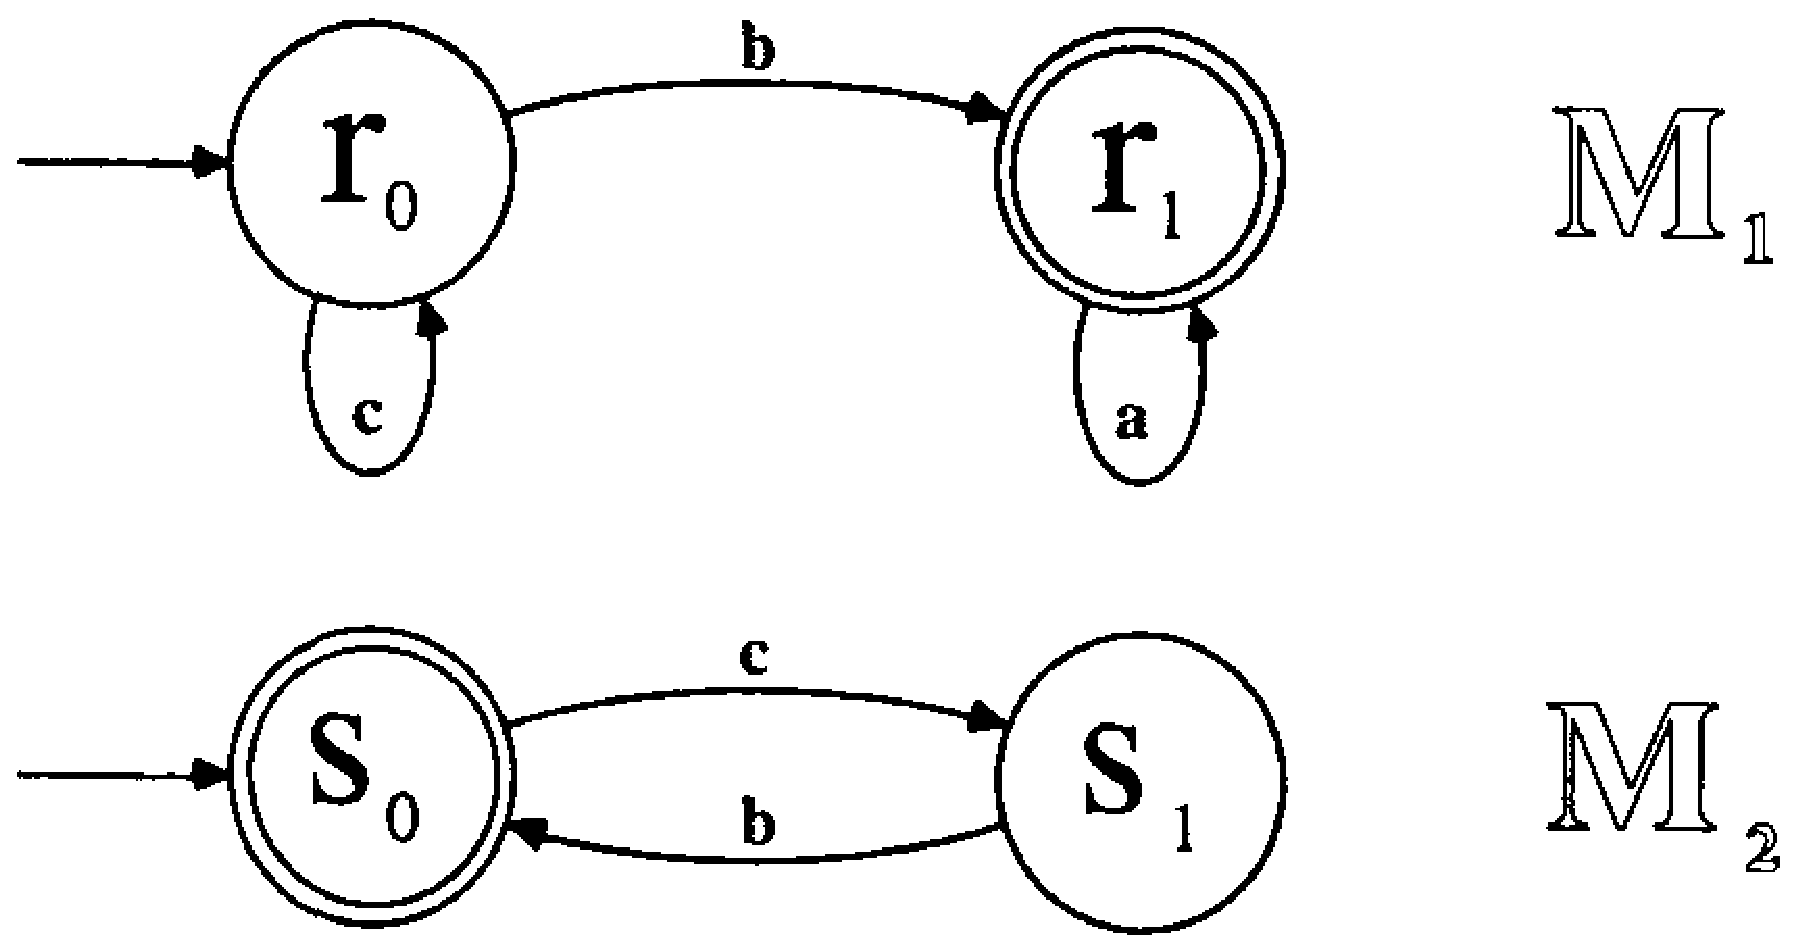
\epsfig{figure=ToFAfigures/fig5-1.eps,width=3in}}
\caption{The two automata discussed in Example 5.6}\label{fig-5.1}
\end{figure}

% Figure 5.2
\begin{figure}
\centerline{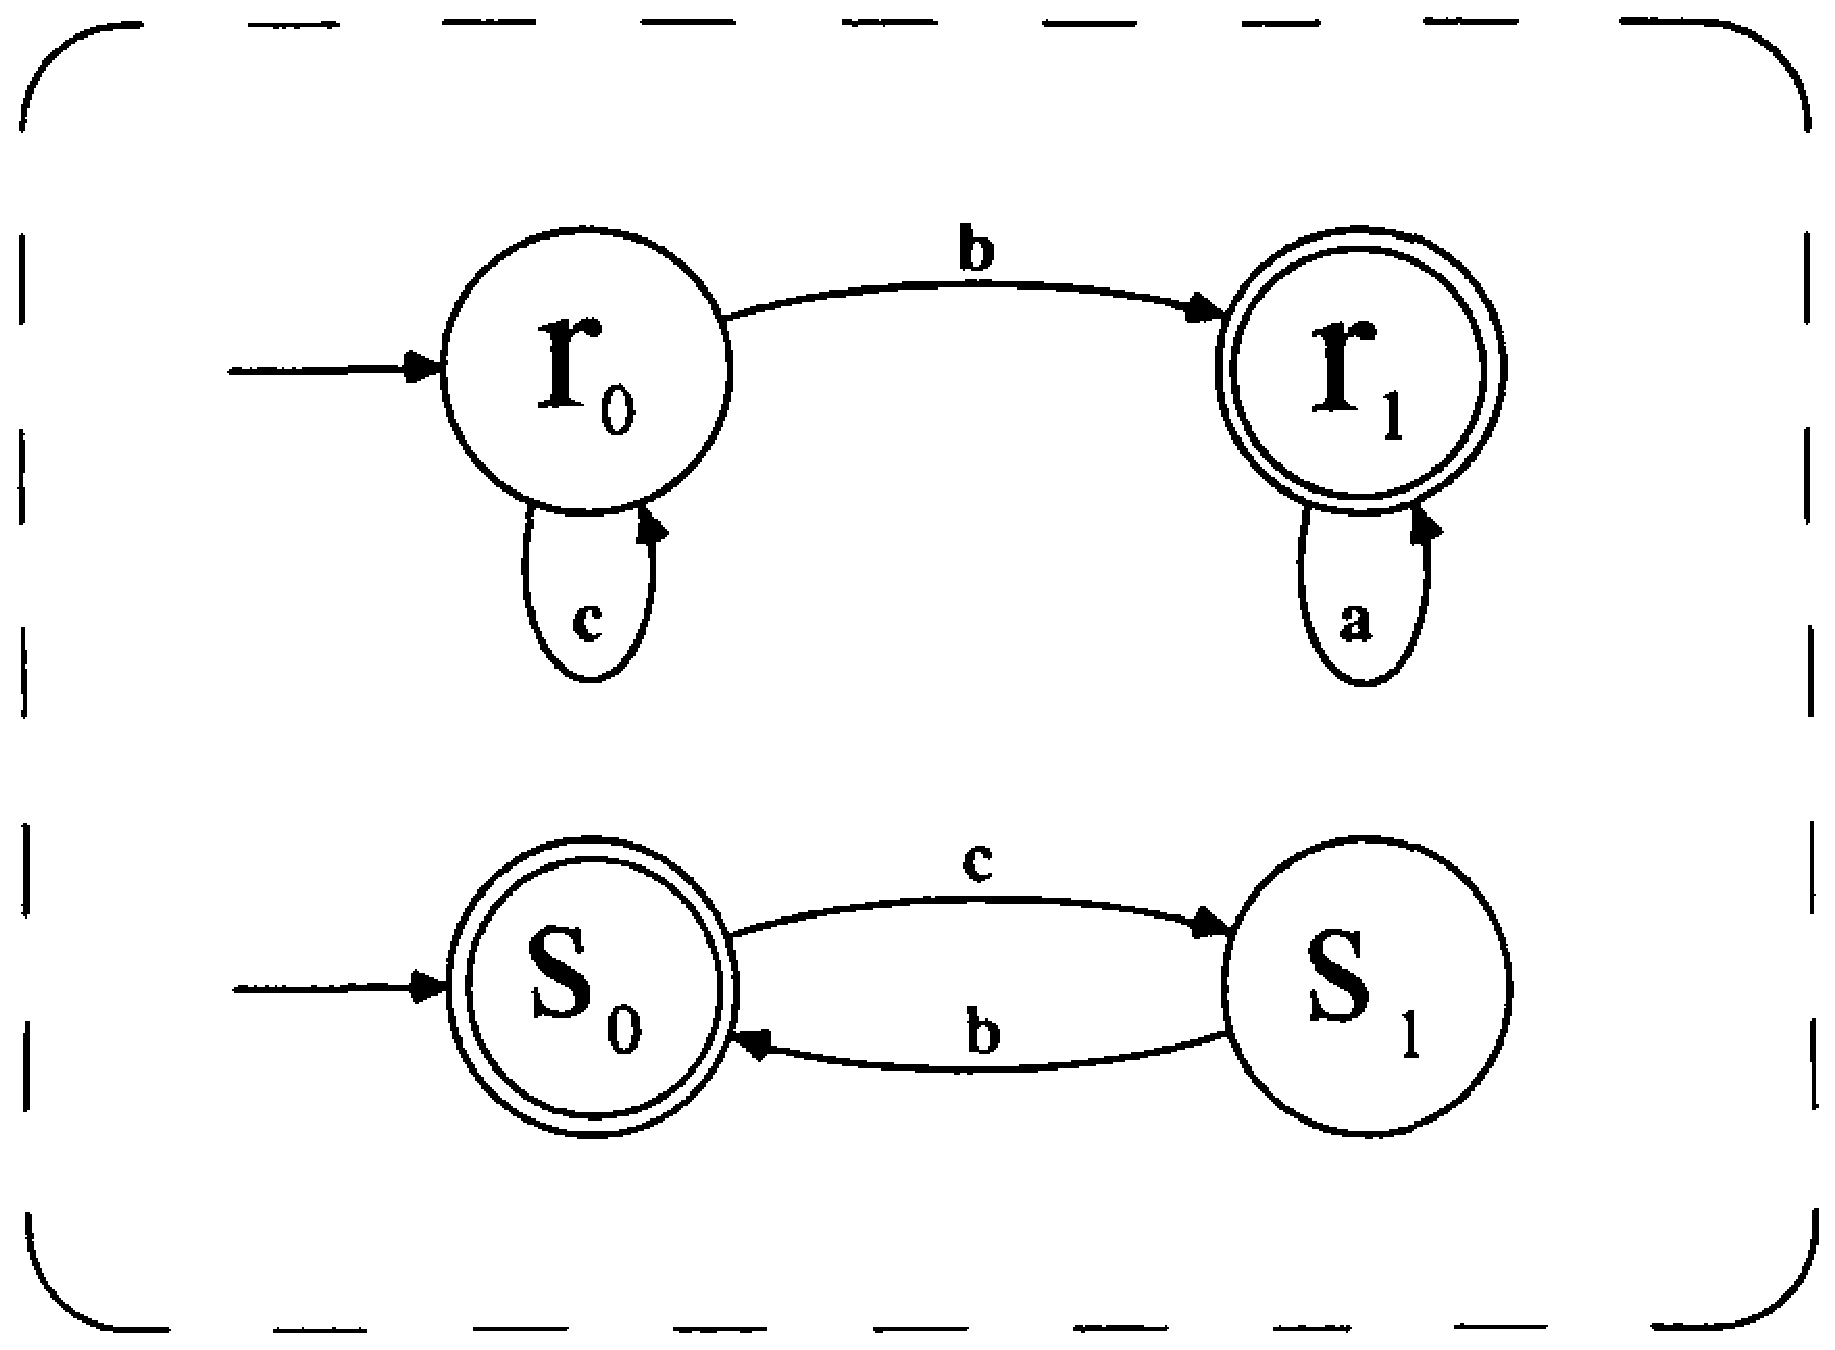
\epsfig{figure=ToFAfigures/fig5-2.eps,width=3in}}
\caption{The resulting automaton in Example 5.6}\label{fig-5.2}
\end{figure}

% Theorem 5.2
\begin{thm}\label{thm-5.2}\index{closure!under union}
For any alphabet $\Sigma$, $\DSIG$ is closed under $\cup$.

\emph{Proof.} Let $L_1$ and $L_2$ belong to $\DSIG$. Then there
are \underline{non}deterministic finite automata
$A_1 =\langle\Sigma,S_1,S_{0_1},\delta_1,F_1\rangle$ and
$A_2 =\langle\Sigma,S_2,S_{0_2},\delta_2,F_2\rangle$ such that $L(A_1)=L_1$ and
$L(A_2)=L_2$ (why?). Define
$A^\cup =\langle\Sigma,S^\cup,S_0^\cup,\delta^\cup,F^\cup\rangle$, where
\begin{center}
\begin{tabular}{ll}
$S^\cup = S_1 \cup S_2$ & (without loss of generality, we can assume
	$S_1 \cap S_2 = \emptyset$) \\
$S_0^\cup = S_{0_1} \cup S_{0_2}$ & \\
$F^\cup = F_1 \cup F_2$ &
\end{tabular}
\end{center}
and $\delta^\cup$$:\ (S_1 \cup S_2) \times \Sigma \rightarrow \wp(S_1 \cup S_2)$ is
defined by
\[ \delta^\cup(s,\pmb{a}) = \left\{\begin{array}{lr}
				\delta_1(s,\pmb{a}) & \text{if }s \in S_1 \\
				& , \\
				\delta_2(s,\pmb{a}) & \text{if }s \in S_2
			     \end{array}\right.
\quad \forall s \in S_1 \cup S_2,\quad \forall \pmb{a} \in \Sigma \]
We claim that $L(A^\cup)=L(A_1) \cup L(A_2)=L_1 \cup L_2$. This must be proved
using the definition of $L$ from Chapter \ref{ch-4}, since $A_1,\ A_2$, and $A^\cup$ are
all NDFAs.
\begin{center}
\begin{tabular}{rcl}
$x \in L(A^\cup)$ & $\Leftrightarrow$ & (from Definition \ref{dfn-4.4}) \\
$(\exists s \in S_0^\cup)[\overline{\delta^\cup}(s,x) \cap F^\cup \not= \emptyset]$ &
	$\Leftrightarrow$ & (by definition of $S_0^\cup$) \\
$(\exists s \in S_{0_1} \cup S_{0_2})[\overline{\delta^\cup}(s,x) \cap F^\cup\not=\emptyset]$
	& $\Leftrightarrow$ & (by definition of $\cup$) \\
$(\exists s \in S_{0_1})[\overline{\delta^\cup}(s,x) \cap F^\cup \not= \emptyset] \vee
	(\exists s \in S_{0_2})[\overline{\delta^\cup}(s,x) \cap F^\cup \not= \emptyset]$ & 
	$\Leftrightarrow$ & (by definition of $\delta^\cup$ and induction) \\
$(\exists s \in S_{0_1})[\DBAR_1(s,x) \cap F^\cup \not= \emptyset] \vee
	(\exists s \in S_{0_2})[\DBAR_2(s,x) \cap F^\cup \not= \emptyset]$ &
	$\Leftrightarrow$ & (by definition of $F^\cup$) \\
$(\exists s \in S_{0_1})[\DBAR_1(s,x) \cap F_1 \not= \emptyset] \vee
	(\exists s \in S_{0_2})[\DBAR_2(s,x) \cap F_2 \not= \emptyset]$ &
	$\Leftrightarrow$ & (from Definition \ref{dfn-4.4}) \\
$x \in L(A_1) \vee x \in L(A_2)$ & $\Leftrightarrow$ &
	(by definition of $\cup$) \\
$x \in (L(A_1) \cup L(A_2))$ & $\Leftrightarrow$ & (by definition of $L_1,L_2$)\\
$x \in L_1 \cup L_2$ &&
\end{tabular}
\end{center}
\end{thm}

The above ``proof'' is actually incomplete; the transition from line 4 to line 5
actually depends on the assumed properties of $\overline{\delta^\cup}$, and not the known
properties of $\delta^\cup$. A rigorous justification should include an
inductive proof of (or at least a reference to) the fact that $\overline{\delta^\cup}$
reflects the same sort of behavior that $\delta^\cup$ does; that is,
\[ \overline{\delta^\cup}(s,x) = \left\{\begin{array}{lr}
				\DBAR_1(s,x) & \text{if }s \in S_1 \\
				& , \\
				\DBAR_2(s,x) & \text{if }s \in S_2
			     \end{array}\right.
\quad \forall s \in S_1 \cup S_2,\quad \forall x \in \Sigma^* \]
The above rule essentially states that the definition that applies to the single
letter $\pmb{a}$ also applies to the string $x$, and it is easy to prove by
induction on the length of $x$ (see the exercises).

The following theorem, which states that $\DSIG$ is closed under
$\cap$, will be justified in two separate ways. The first proof will argue that
the closure property must hold due to previous results; no new DFA need be
constructed. The drawback to this type of proof is that we have no suitable
guide for actually combining two existing DFAs into a new machine that will
recognize the appropriate intersection (although, as outlined in the exercises,
in this case a construction based on the first proof is fairly easy to generate).

Some operators are so bizarre that a nonconstructive proof of closure is the
best we can hope for; intersection is definitely \emph{not} that strange,
however. In a second proof of the closure of $\DSIG$ under $\cap$,
Lemma \ref{lmm-5.1} will explicitly outline how an intersection machine could be built.
When such constructions can be demonstrated, we will say that
$\DSIG$ is \emph{effectively} closed under the operator in
question (see Theorem \ref{thm-5.12} for a discussion of an operator that is not
effectively closed).

% Theorem 5.3
\begin{thm}\label{thm-5.3}\index{closure!under intersection}
For any alphabet $\Sigma$, $\DSIG$ is closed under $\cap$.

\emph{Proof.} Let $L_1$ and $L_2$ belong to $\DSIG$. Then by
Theorem \ref{thm-5.1}, $\sim\!\! L_1$ and $\sim\!\! L_2$ are also FAD. By Theorem \ref{thm-5.2},
$\sim\!\! L_1 \cup \sim\!\! L_2$ is also FAD. By Theorem \ref{thm-5.1} again,
$\sim\!\!(\sim\!\! L_1 \cup \sim\!\! L_2)$ is also FAD. By De Morgan's law, this
last expression is equivalent to $L_1 \cap L_2$, so $L_1 \cap L_2$ is FAD, and
thus $L_1 \cap L_2 \in \DSIG$.
\end{thm}

Note that the above argument could be made to apply to \emph{any} collection C
of sets that were known to be closed under union and complementation. A second
proof of Theorem \ref{thm-5.3} might rely on the following lemma, using the ``direct''
method of constructing a deterministic machine that accepts $L_1 \cap L_2$. This
would show that $\DSIG$ is \emph{effectively} closed under the
intersection operator.

% Lemma 5.1
\begin{lmm}\label{lmm-5.1}\index{closure!under intersection}\index{cross product}
Given \emph{deterministic} finite automata
$A_1 =\langle\Sigma,S_1,s_{0_1},\delta_1,F_1\rangle$ and
$A_2 =\langle\Sigma,S_2,s_{0_2},\delta_2,F_2\rangle$ such that $L(A_1)=L_1$, and
$L(A_2) = L_2$, define a new DFA
$A^\cap =\langle\Sigma,S^\cap,s_0^\cap,\delta^\cap,F^\cap\rangle$, where
\begin{center}
\begin{tabular}{l}
$S^\cap = S_1 \times S_2$ \\
$s_0^\cap = \langle s_{0_1},s_{0_2}\rangle$ \\
$F^\cap = F_1 \times F_2$
\end{tabular}
\end{center}
and $\delta^\cap$$:\ (S_1 \times S_2) \times \Sigma \rightarrow S_1 \times S_2$ is
defined by
\[ \delta^\cap(\langle s,t\rangle,\pmb{a}) = \langle\delta_1(s,\pmb{a}),\delta_2(t,\pmb{a})\rangle\quad
	\forall s \in S_1, \forall t \in S_2, \forall \pmb{a} \in \Sigma \]
Then $L(A^\cap) = L_1 \cap L_2.$

\emph{Proof.} As usual, the key is to show that
$x \in L(A^\cap) \Leftrightarrow x \in L_1 \cap L_2$. The proof hinges on the
inductive statement that $\overline{\delta^\cap}$ obeys the same rule that defines
$\delta^\cap$; that is,
$(\forall s \in S_1)(\forall t \in S_2)(\forall x \in \Sigma^*)
[\overline{\delta^\cap}(\langle s,t\rangle,x)=\langle\DBAR_1(s,x),\DBAR_2(t,x)\rangle]$. The details are left for the
reader (see the exercises).
\end{lmm}

% Figure 5.3
\begin{figure}
\centerline{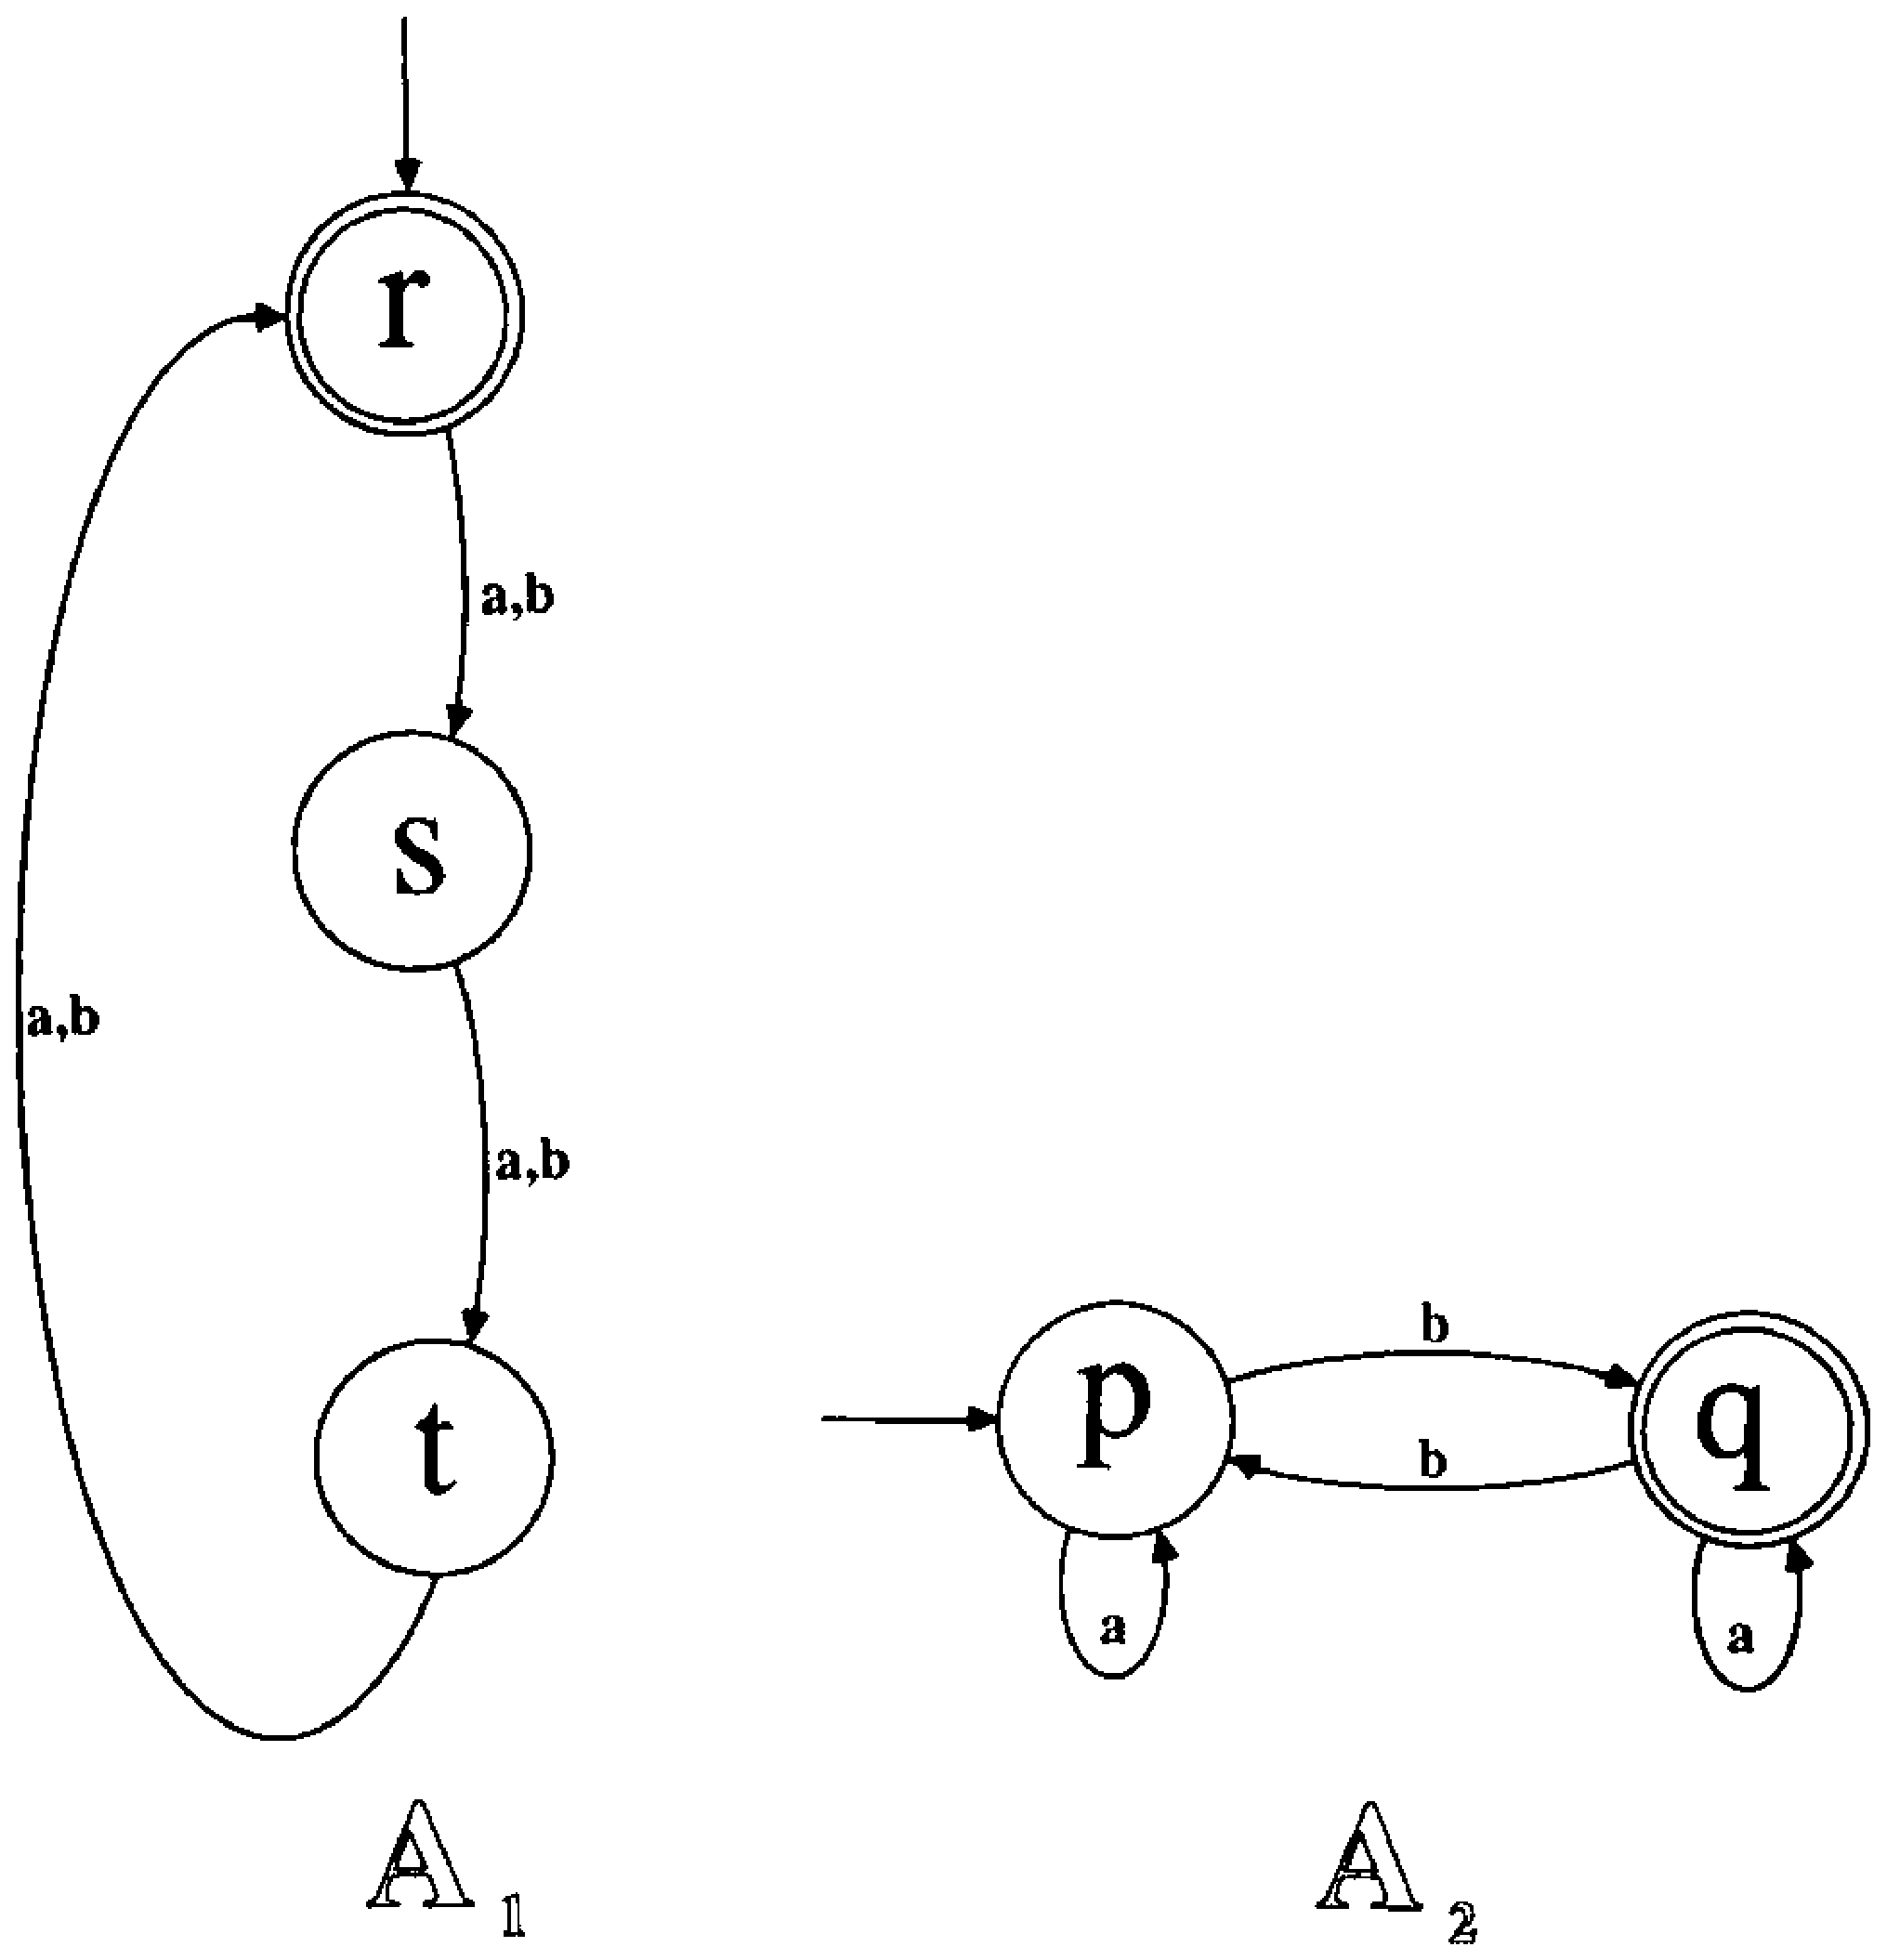
\epsfig{figure=ToFAfigures/fig5-3.eps,height=3.6in}}
\caption{The automata discussed in Example 5.7}\label{fig-5.3}
\end{figure}

The idea behind the above construction is to build a machine that ``remembers''
the state changes that both $A_1$ and $A_2$ make as they each process the same
string, and hence the state set consists of all possible pairs of states from
$A_1$ and $A_2$. The goal was to design the transition function $\delta^\cap$ so
that being in state $\langle s,t\rangle$ in $A^\cap$ indicates that $A_1$ would
currently be in state $s$ and $A_2$ would be in state $t$. This goal also
motivates the definition of the new start state; we want to begin in the start
states of $A_1$ and $A_2$, and hence $s_0^\cap =\langle s_{0_1},s_{0_2}\rangle$.
We only wish to accept strings that are common to both languages, which means
that the terminating state in $A_1$ belongs to $F_1$ and the last state reached
in $A_2$ is likewise a final state. This requirement naturally leads to the
definition of $F^\cap$, where $\langle s,t\rangle$ is a final state if and only
if both $s$ and $t$ were final states in their respective machines.

\subsection*{Example 5.7}

Consider the two machines $A_1$ and $A_2$ displayed in Figure \ref{fig-5.3}. Note that
$A_2$ ``remembers'' whether there have been an even or an odd number of
$\pmb{b}$s, while $A_1$ ``counts'' the number of letters ($\bmod{ 3}$). We now
demonstrate how the definition in Lemma \ref{lmm-5.1} can be applied to form a
deterministic machine that accepts the intersection of $L(A_1)$ and $L(A_2)$.
The structure of $A^\cap$ would in this case look like the automaton shown in
Figure \ref{fig-5.4}. Note that $A^\cap$ does indeed keep track of the criteria that both
$A_1$ and $A_2$ use to accept or reject strings. We will be in a state on the
right side of $A^\cap$ if an odd number of $\pmb{b}$s have been seen and on the
left side when an even number of $\pmb{b}$s have been processed. At the same time,
we will be in the upper, middle, or lower row of states depending on the total
number of letters$\pmod{3}$ that have been processed. There is but one final
state, corresponding to the situation where we have both an odd number of
$\pmb{b}$s and the letter count is $0 \pmod{ 3}$.

% Figure 5.4
\begin{figure}
\centerline{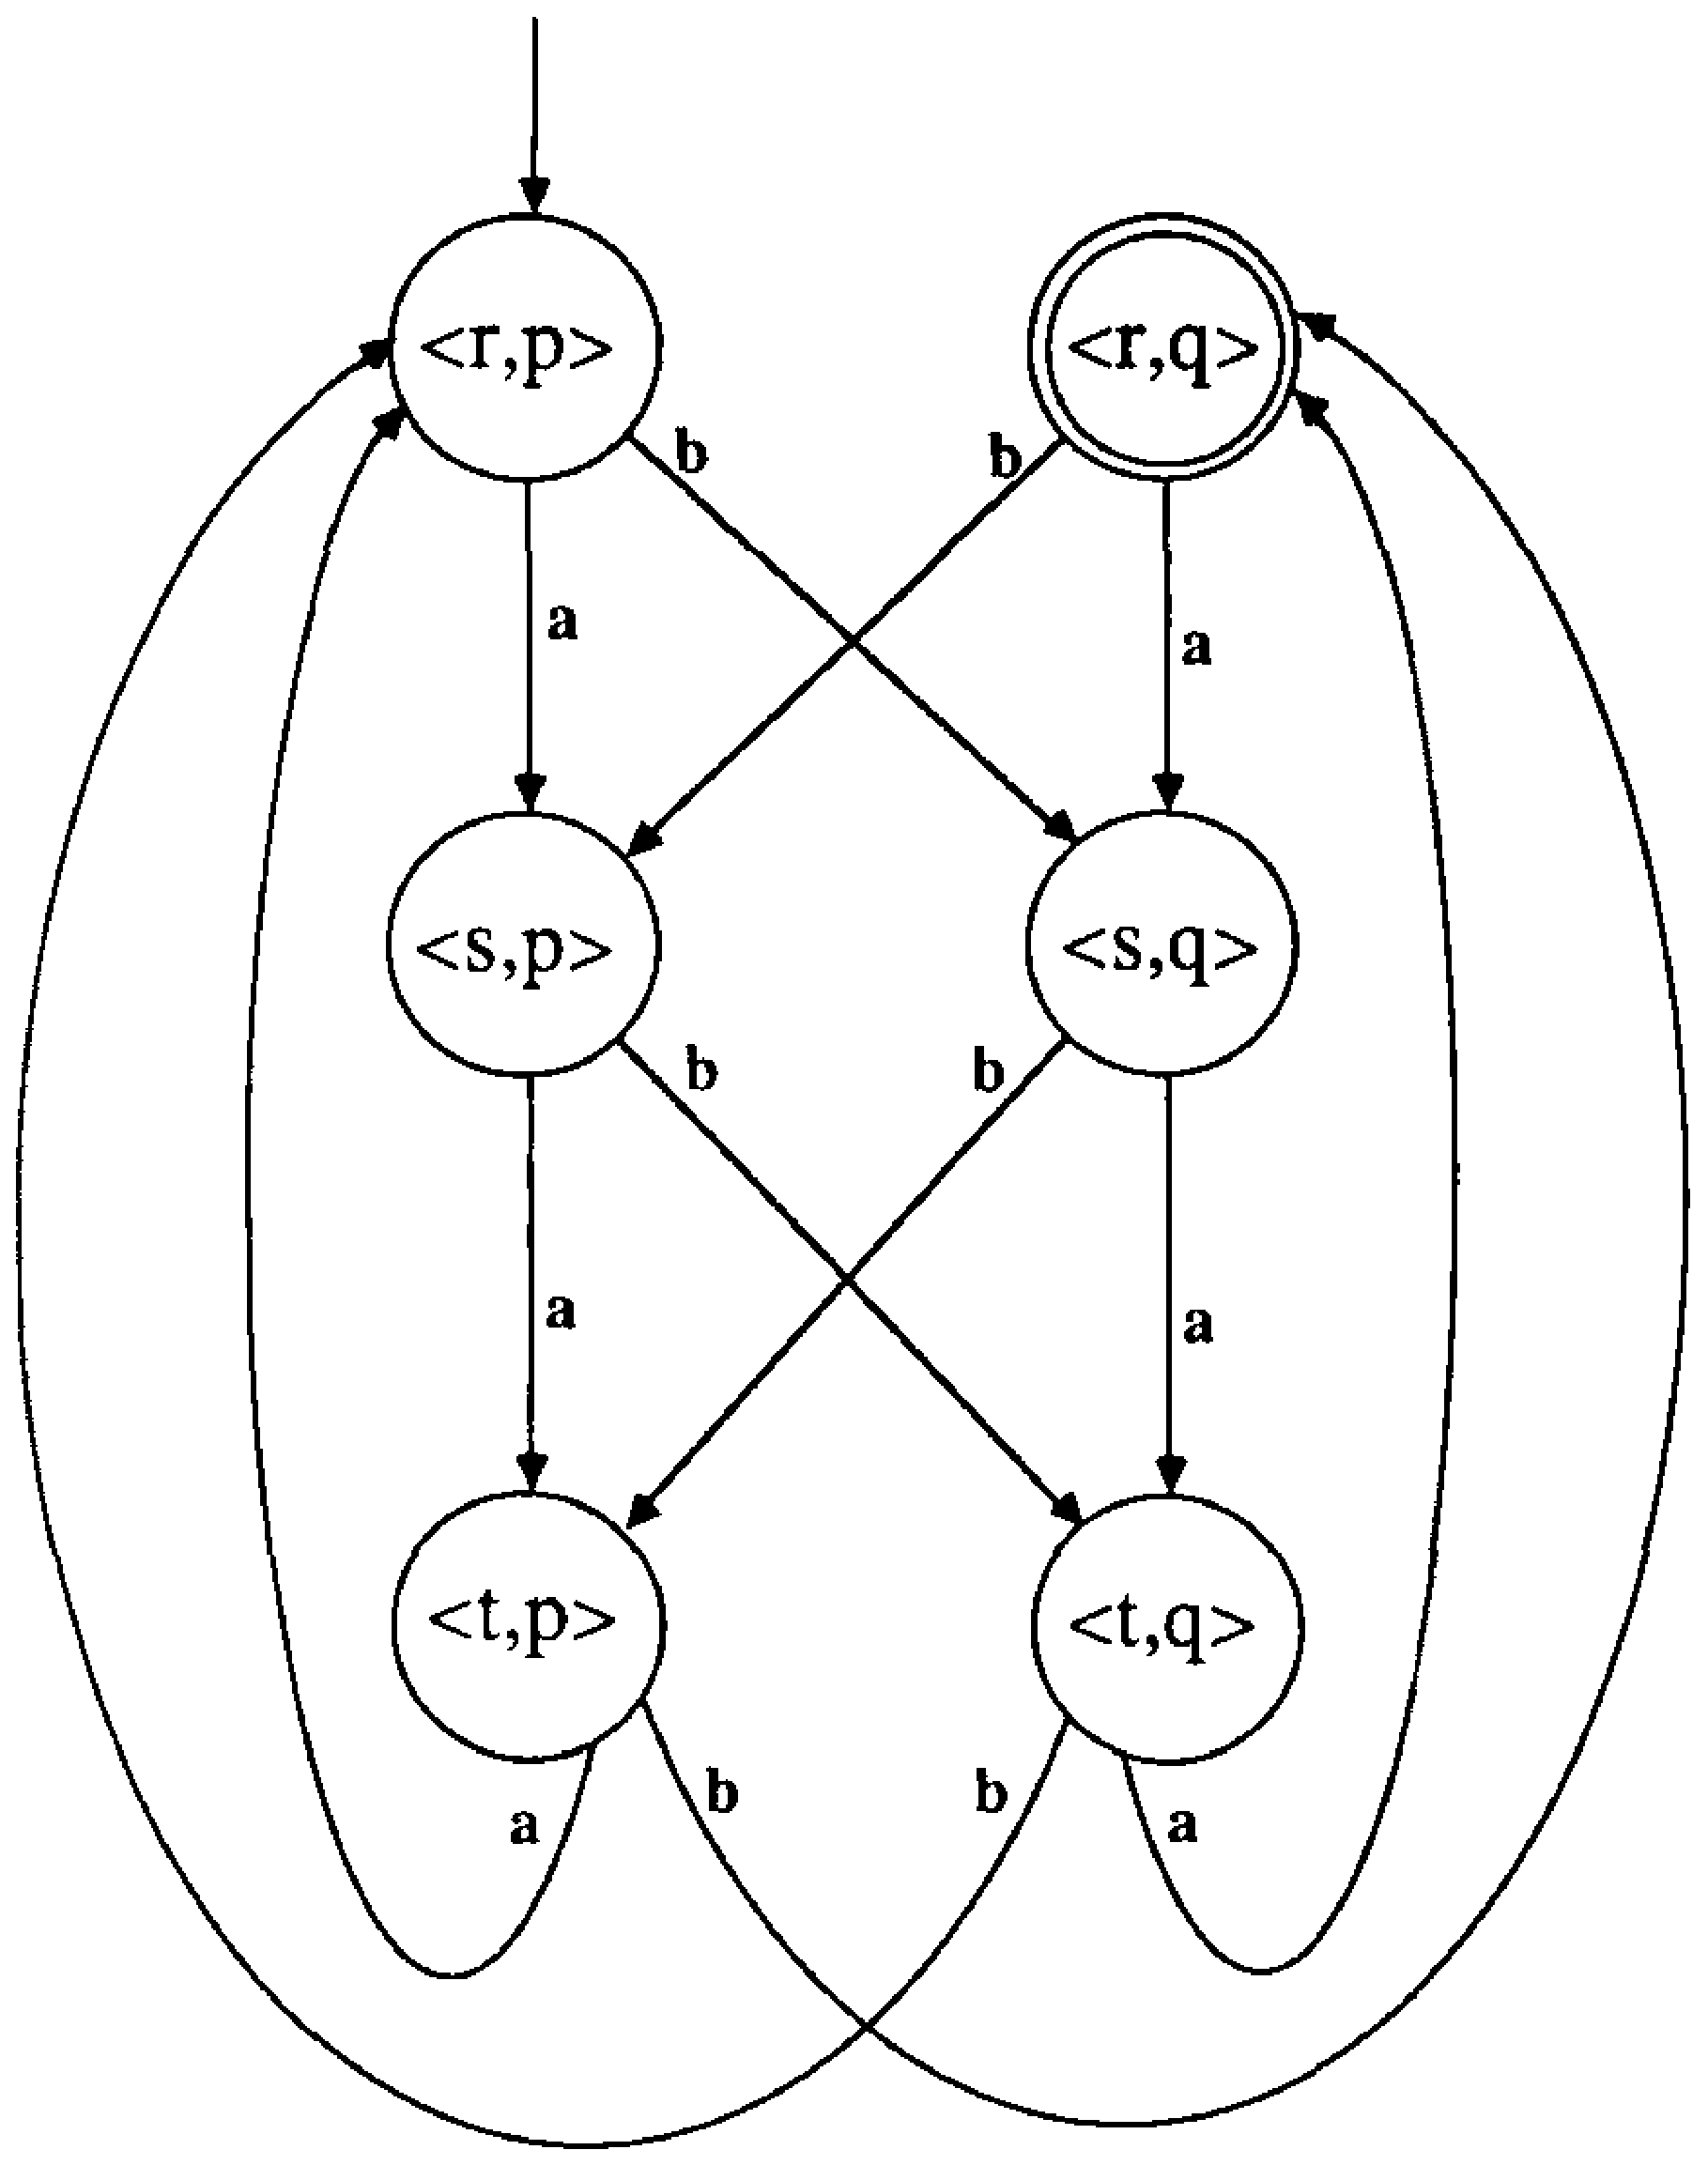
\epsfig{figure=ToFAfigures/fig5-4.eps,height=3.6in}}
\caption{The resulting DFA for Example 5.7}\label{fig-5.4}
\end{figure}

The operations used in the previous three theorems are common to set theory. We
now present some new operators that are special to string algebra. We have
defined concatenation $(\cdot)$ for individual strings, but there is a natural
extension of the definition to languages, as indicated by the next definition.

% Definition 5.4
\begin{dfn}\label{dfn-5.4}\index{concatenation!of languages}
Let $L_1$ and $L_2$ be languages. The \emph{concatenation} of $L_1$ with
$L_2$, written $L_1 \cdot L_2$, is defined by
\[ L_1 \cdot L_2 =\{x\cdot y\ |\ x \in L_1 \wedge y \in L_2\} \]
\end{dfn}

\subsection*{Example 5.8}

If $L_1 =\{\lambda,\pmb{b},\pmb{cc}\}$ and $L_2=\{\lambda,\pmb{aa},\pmb{baa}\}$,
then
\[ L_1 \cdot L_2 =\{\lambda, \pmb{b},\pmb{cc},\pmb{aa},\pmb{baa},\pmb{ccaa},
	\pmb{bbaa},\pmb{ccbaa}\}. \]

Note that $\pmb{baa}$ qualifies to be in $L_1\cdot L_2$ for two reasons:
$\pmb{baa} = \lambda \cdot \pmb{baa}$ and $\pmb{baa} = \pmb{b} \cdot \pmb{aa}$.
Thus we see that the concatenation contains only eight words rather than the
expected $9( = 3\cdot 3)$. In general, $L_1 \cdot L_2$ consists of all words
that can be formed by the concatenation of a word from $L_1$ with a word from
$L_2$; for finite sets, concatenating an $n$ word set with an $m$ word set
results in no more than $n \cdot m$ words. As shown in this example, the number
of words can actually be less than $n \cdot m$. Larger languages can be
concatenated, also. For example, $\Sigma^* \cdot \Sigma = \Sigma^+$.

The concatenation of two FAD languages is also FAD, as can easily be seen by
employing NDFAs with $\lambda$-transitions.

\subsection*{Example 5.9}

Figure \ref{fig-5.5} illustrates two nondeterministic finite automata $B_1$ and $B_2$ that
accept the languages $L_1$ and $L_2$ given in Example 5.8. Combining these two
machines and linking the final states of $B_1$ to the start states of $B_2$ with
$\lambda$-transitions yields a new NDFA that accepts $L_1 \cdot L_2$, as shown
in Figure \ref{fig-5.6}.

% Figure 5.5
\begin{figure}
\centerline{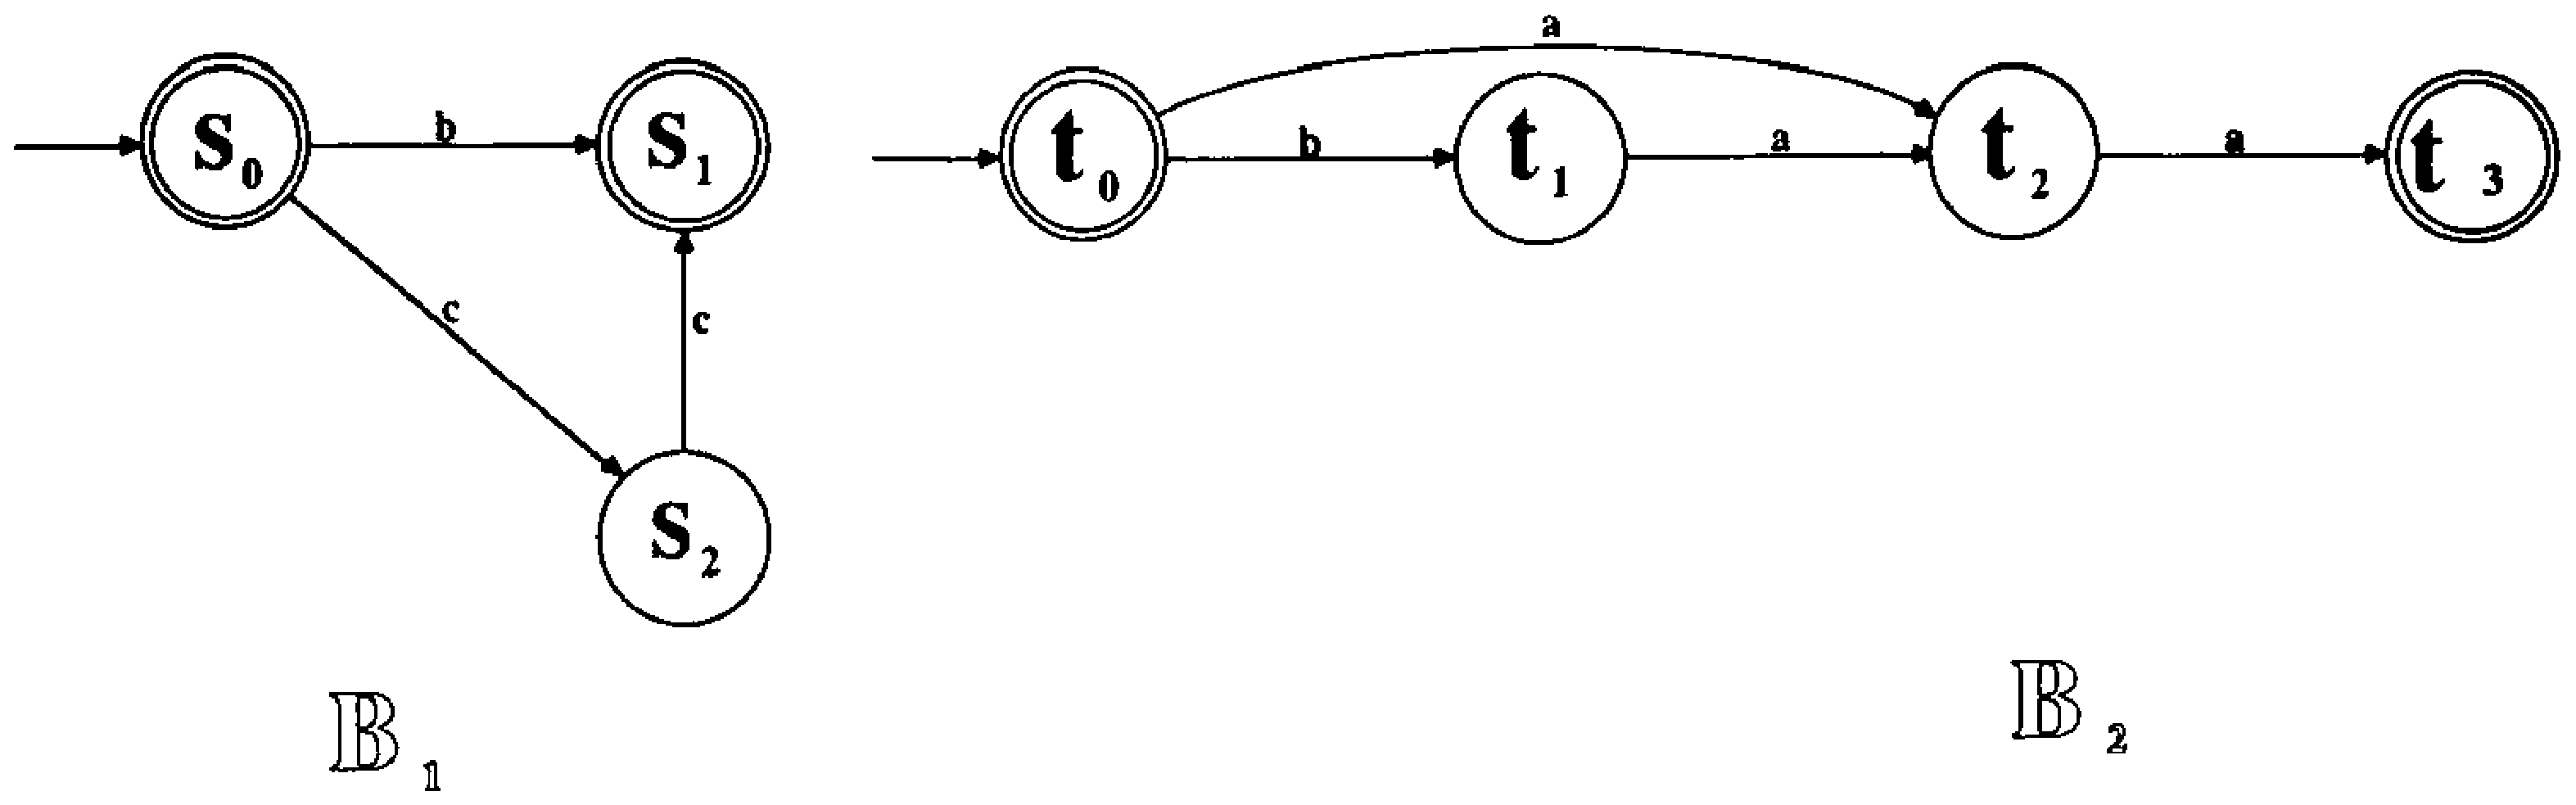
\epsfig{figure=ToFAfigures/fig5-5.eps,width=6in}}
\caption{Two candidates for concatenation}\label{fig-5.5}
\end{figure}

% Figure 5.6
\begin{figure}
\centerline{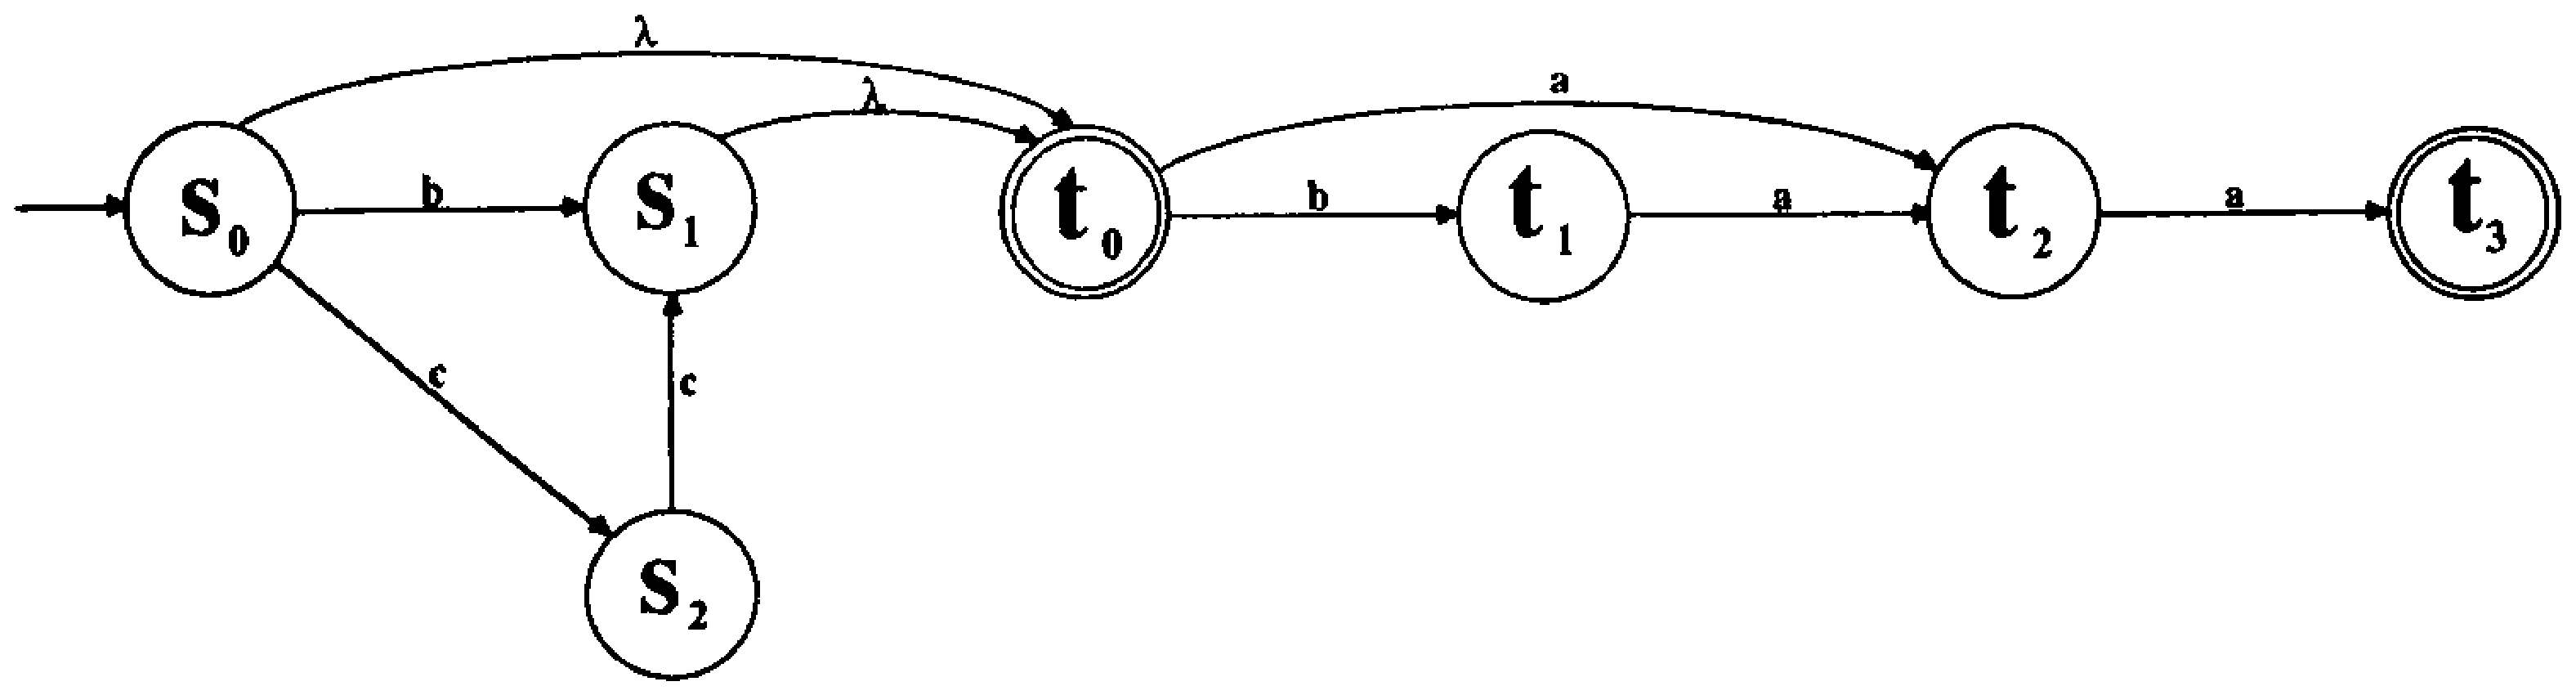
\epsfig{figure=ToFAfigures/fig5-6.eps,width=6in}}
\caption{An NDFA which accepts the concatenation of the machines discussed in
Example 5.9}\label{fig-5.6}
\end{figure}

\subsection*{Example 5.10}

Consider the \emph{deterministic} finite automata $A_1$ and $A_2$ displayed in
Figure \ref{fig-5.7}. These can similarly be linked together to form an NDFA that accepts
the concatenation of the languages accepted by $A_1$ and $A_2$, as shown in
Figure \ref{fig-5.8}.

% Figure 5.7
\begin{figure}
\centerline{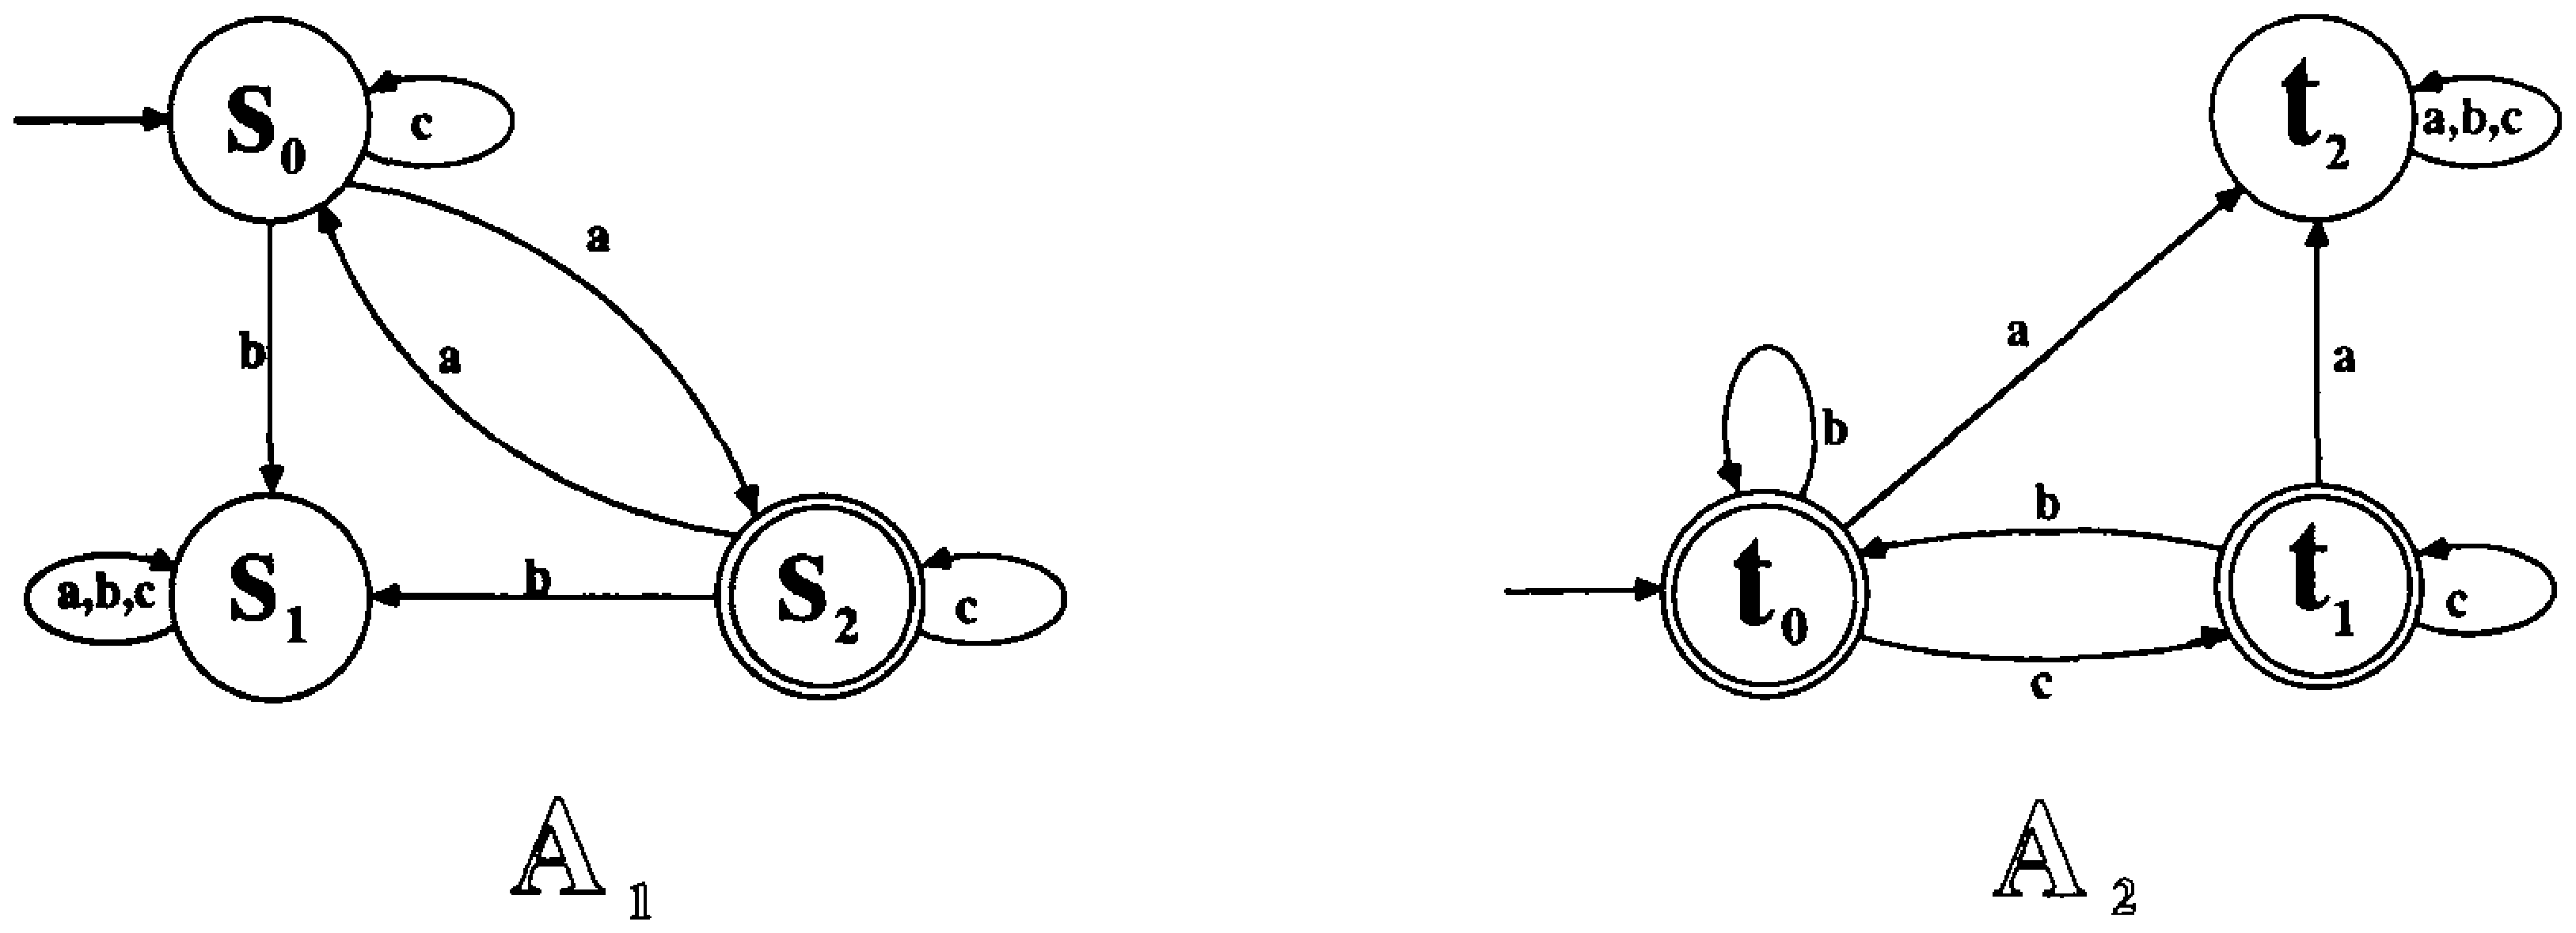
\epsfig{figure=ToFAfigures/fig5-7.eps,width=6in}}
\caption{A pair of candidates for concatenation}\label{fig-5.7}
\end{figure}

% Figure 5.8
\begin{figure}
\centerline{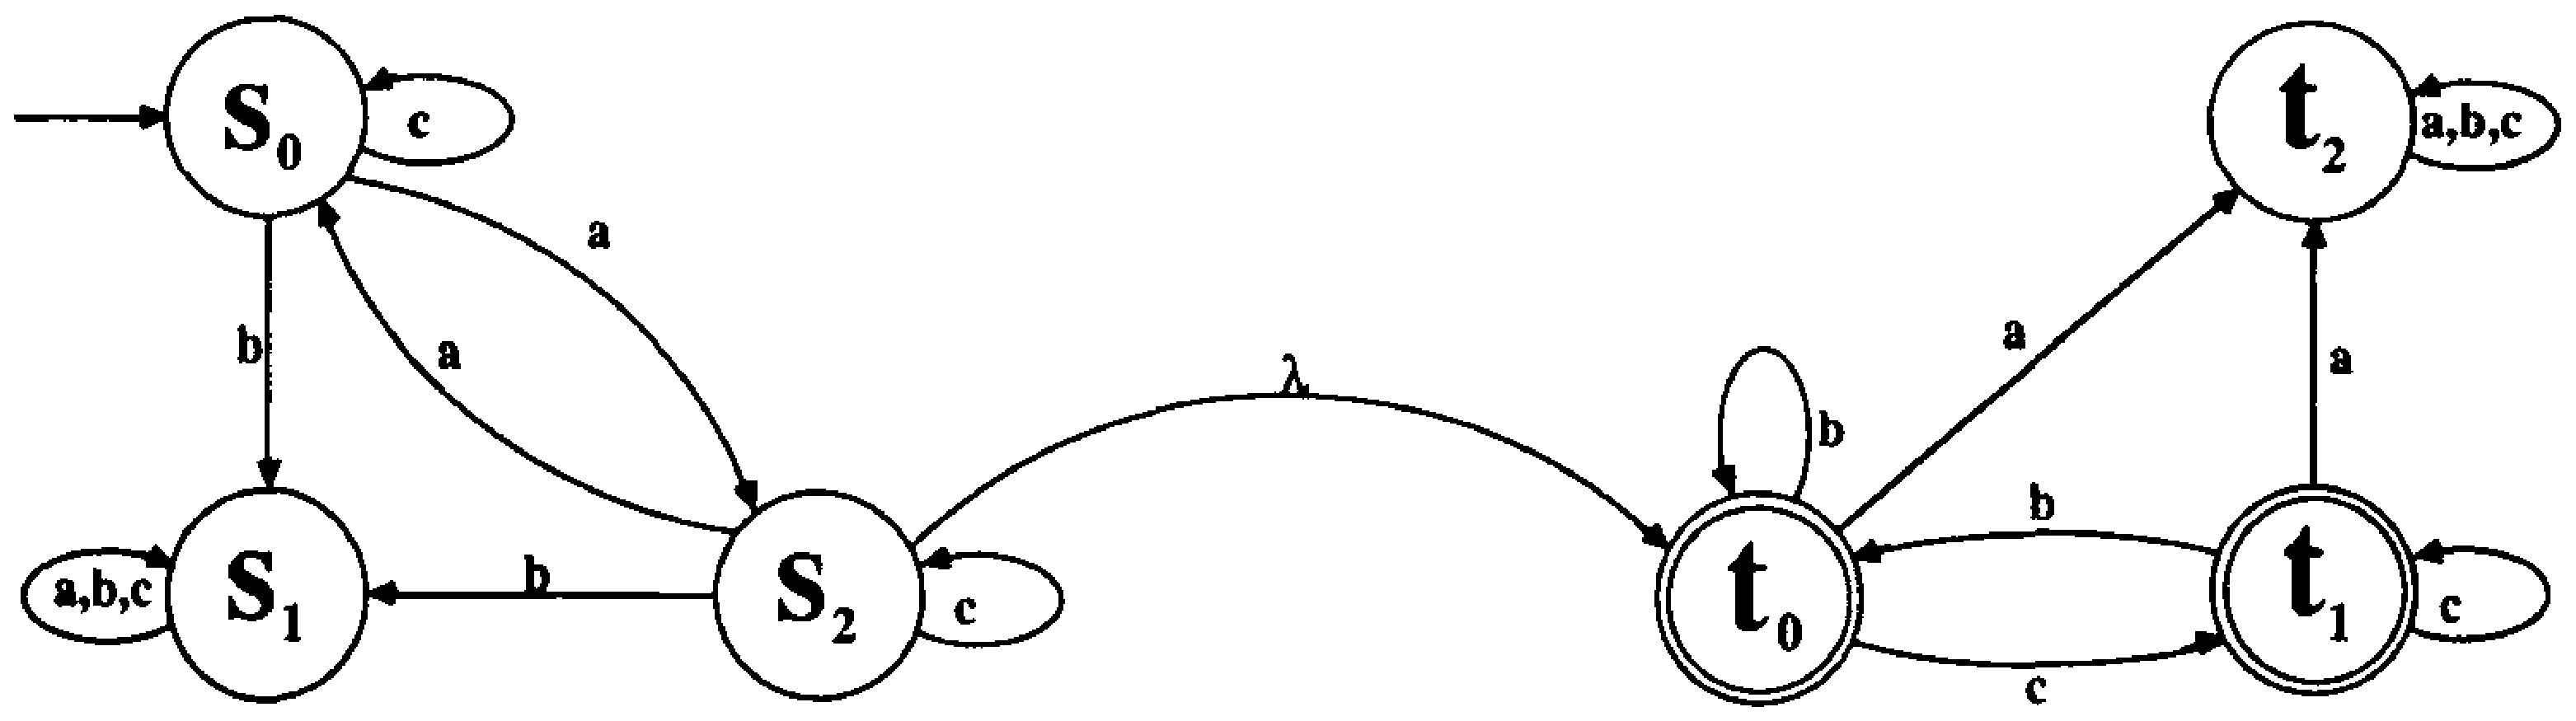
\epsfig{figure=ToFAfigures/fig5-8.eps,width=6in}}
\caption{Concatenation of the machines in Example 5.10 via lambda-moves}\label{fig-5.8}
\end{figure}

It is also possible to directly build a machine for concatenation without using
any $\lambda$-transitions, although the penalty for limiting our attention to
less exotic machines is a loss of clarity in the construction. While the proof
of the following theorem does not depend on $\lambda$-transitions, the resulting
machine is still nondeterministic.

% Theorem 5.4
\begin{thm}\label{thm-5.4}\index{closure!under concatenation}
For any alphabet $\Sigma$, $\DSIG$ is closed under $\cdot$
(concatenation).

\emph{Proof.} Let $L_1$ and $L_2$ belong to $\DSIG$. Then there
are \underline{deterministic} finite automata
$A_1=\langle\Sigma,S_1,s_{0_1},\delta_1,F_1\rangle$ and
$A_2=\langle\Sigma,S_2,s_{0_2},\delta_2,F_2\rangle$ such that $L(A_1)=L_1$ and
$L(A_2)=L_2$. Without loss of generality, assume $S_1 \cap S_2 = \emptyset$.
Define a \underline{non}deterministic machine
$A^\bullet =\langle\Sigma,S^\bullet,S_0^\bullet,\delta^\bullet,F^\bullet\rangle$, where
\begin{center}
\begin{tabular}{ll}
$S^\bullet = S_1 \cup S_2$ & \\ %(without loss of generality, assume
%	$S_1 \cap S_2 = \emptyset$) \\
$S_0^\bullet =\{s_{0_1}\}$ & \\
$F^\bullet = \left\{\begin{array}{l}
			F_2 \\
			F_1 \cup F_2
		  \end{array}\right.$
	& $\begin{array}{l}
		\text{if }\lambda \notin L_2 \\
		\text{if }\lambda \in L_2
	  \end{array}$
\end{tabular}
\end{center}
and $\delta^\bullet$$: (S_1 \cup S_2) \times \Sigma \rightarrow \wp(S_1 \cup S_2)$
is defined by
\begin{center}
\begin{tabular}{l}
$\delta^\bullet(s,\pmb{a})=\left\{\begin{array}{ll}
		\{\delta_1(s,\pmb{a})\} & \text{if }s \in S_1 - F_1 \\
		\{\delta_1(s,\pmb{a}),\delta_2(s_{0_2},\pmb{a})\} & \text{if }s\in F_1 \\
		\{\delta_2(s,\pmb{a})\} & \text{if }s \in S_2
		\end{array}\right.$
\end{tabular}
\end{center}
It can be shown that $L(A^\bullet)=L(A_1)\cdot L(A_2)=L_1 \cdot L_2$ (see the
exercises).
\end{thm}

\subsection*{Example 5.11}

Consider the deterministic finite automata $A_1$ and $A_2$ in Example 5.10. These
can be linked together to form the NDFA $A^\cdot$, and the reader can indeed
verify that the machine illustrated in Figure \ref{fig-5.9} accepts the concatenation of
the languages accepted by $A_1$ and $A_2$. Notice that the new transitions from
the final states of $A_1$ mimic the transitions out of the start state of $A_2$.

Thus we see that avoiding $\lambda$-transitions while defining a concatenation
machine is relatively simple. Unfortunately, avoiding the nondeterministic
aspects of the construction is relatively impractical and would basically entail
re-creating the construction in Definition \ref{dfn-4.5} (which outlined the method for
converting an NDFA into a DFA). Whereas it was merely convenient (rather than
necessary) to employ NDFAs to demonstrate that $\DSIG$ is closed
under union, the use of nondeterminism is essential to the proof of closure
under concatenation.

% Figure 5.9
\begin{figure}
\centerline{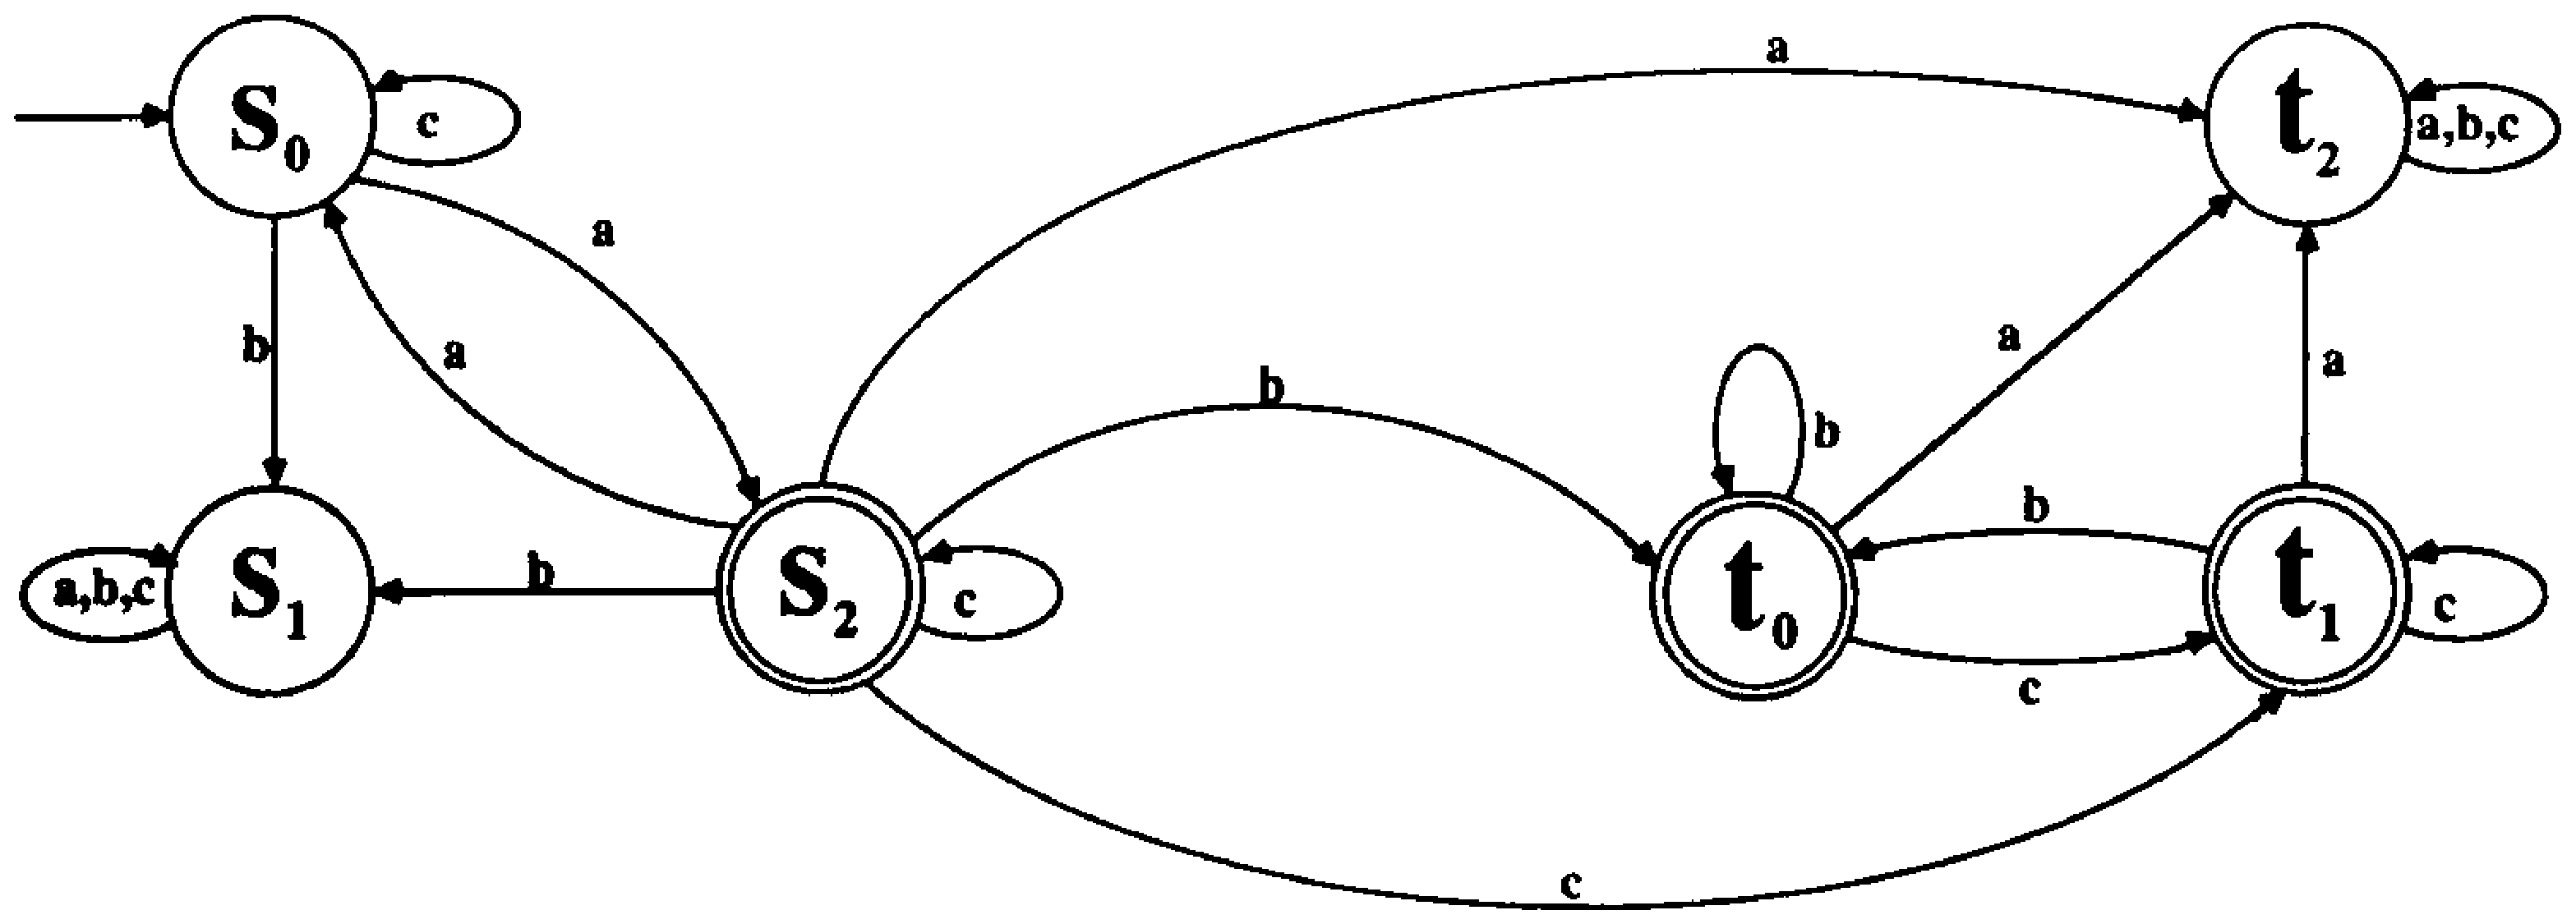
\epsfig{figure=ToFAfigures/fig5-9.eps,width=6in}}
\caption{Concatenation of the machines in Example 5.10 without lambda-moves
(Example 5.11)}\label{fig-5.9}
\end{figure}

\subsection*{Example 5.12}

Consider the nondeterministic finite automata $B_1$ and $B_2$ from Example 5.9.
Applying the analog of Theorem \ref{thm-5.4} (see Exercise 5.43) yields the automaton
shown in Figure \ref{fig-5.10}. Notice that each final state of $B_1$ now also mimics the start
state of $B_2$, and $t_0$ has become a disconnected state. Both $s_0$ and $s_1$
are still final states since $\lambda \in L(B_2)$.

\subsection*{Example 5.13}

Consider the nondeterministic finite automata $B_1$ and $B_3$ shown in Figure
\ref{fig-5.11}, where $B_1$ is the same as that given in Example 5.9, while $B_3$ differs
just slightly from $B_2$ ($t_0$ is no longer a final state). Note that
$L(B_3)=\{\pmb{aa},\pmb{baa}\}$, and $\lambda \notin L(B_3)$. Applying Theorem
\ref{thm-5.4} in this case yields the automaton shown in Figure \ref{fig-5.12}. In this
construction, $s_0$ and $s_1$ are no longer final states since the definition of
$F$ must follow a different rule when $\lambda \notin L(B_3)$. By examining the
resulting machine, the reader can verify that having $t_3$ as the only final
state is indeed the correct strategy for this case.

% Figure 5.10
\begin{figure}
\centerline{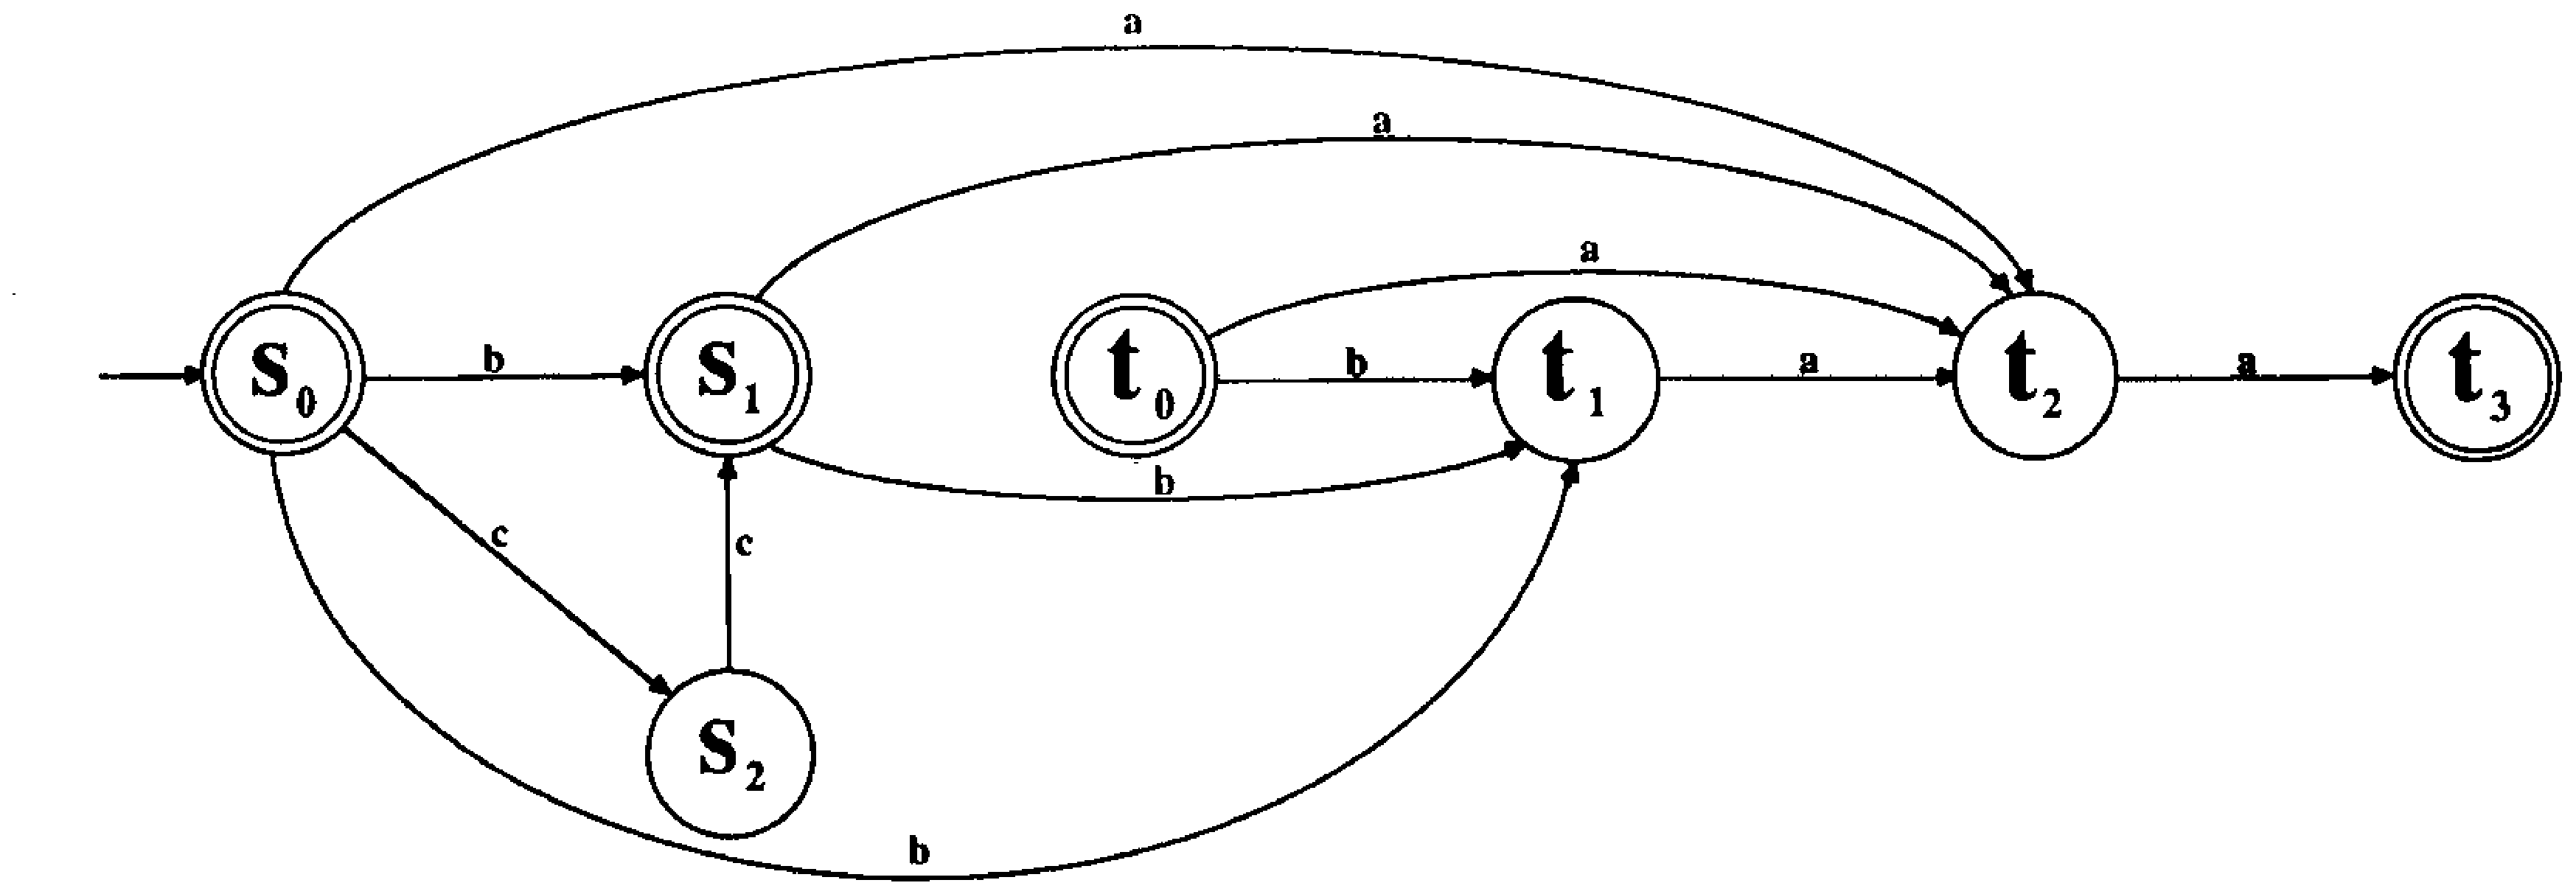
\epsfig{figure=ToFAfigures/fig5-10.eps,width=6in}}
\caption{An NDFA without lambda-moves which accepts the concatenation of the
languages discussed in Example 5.8}\label{fig-5.10}
\end{figure}

% Figure 5.11
\begin{figure}
\centerline{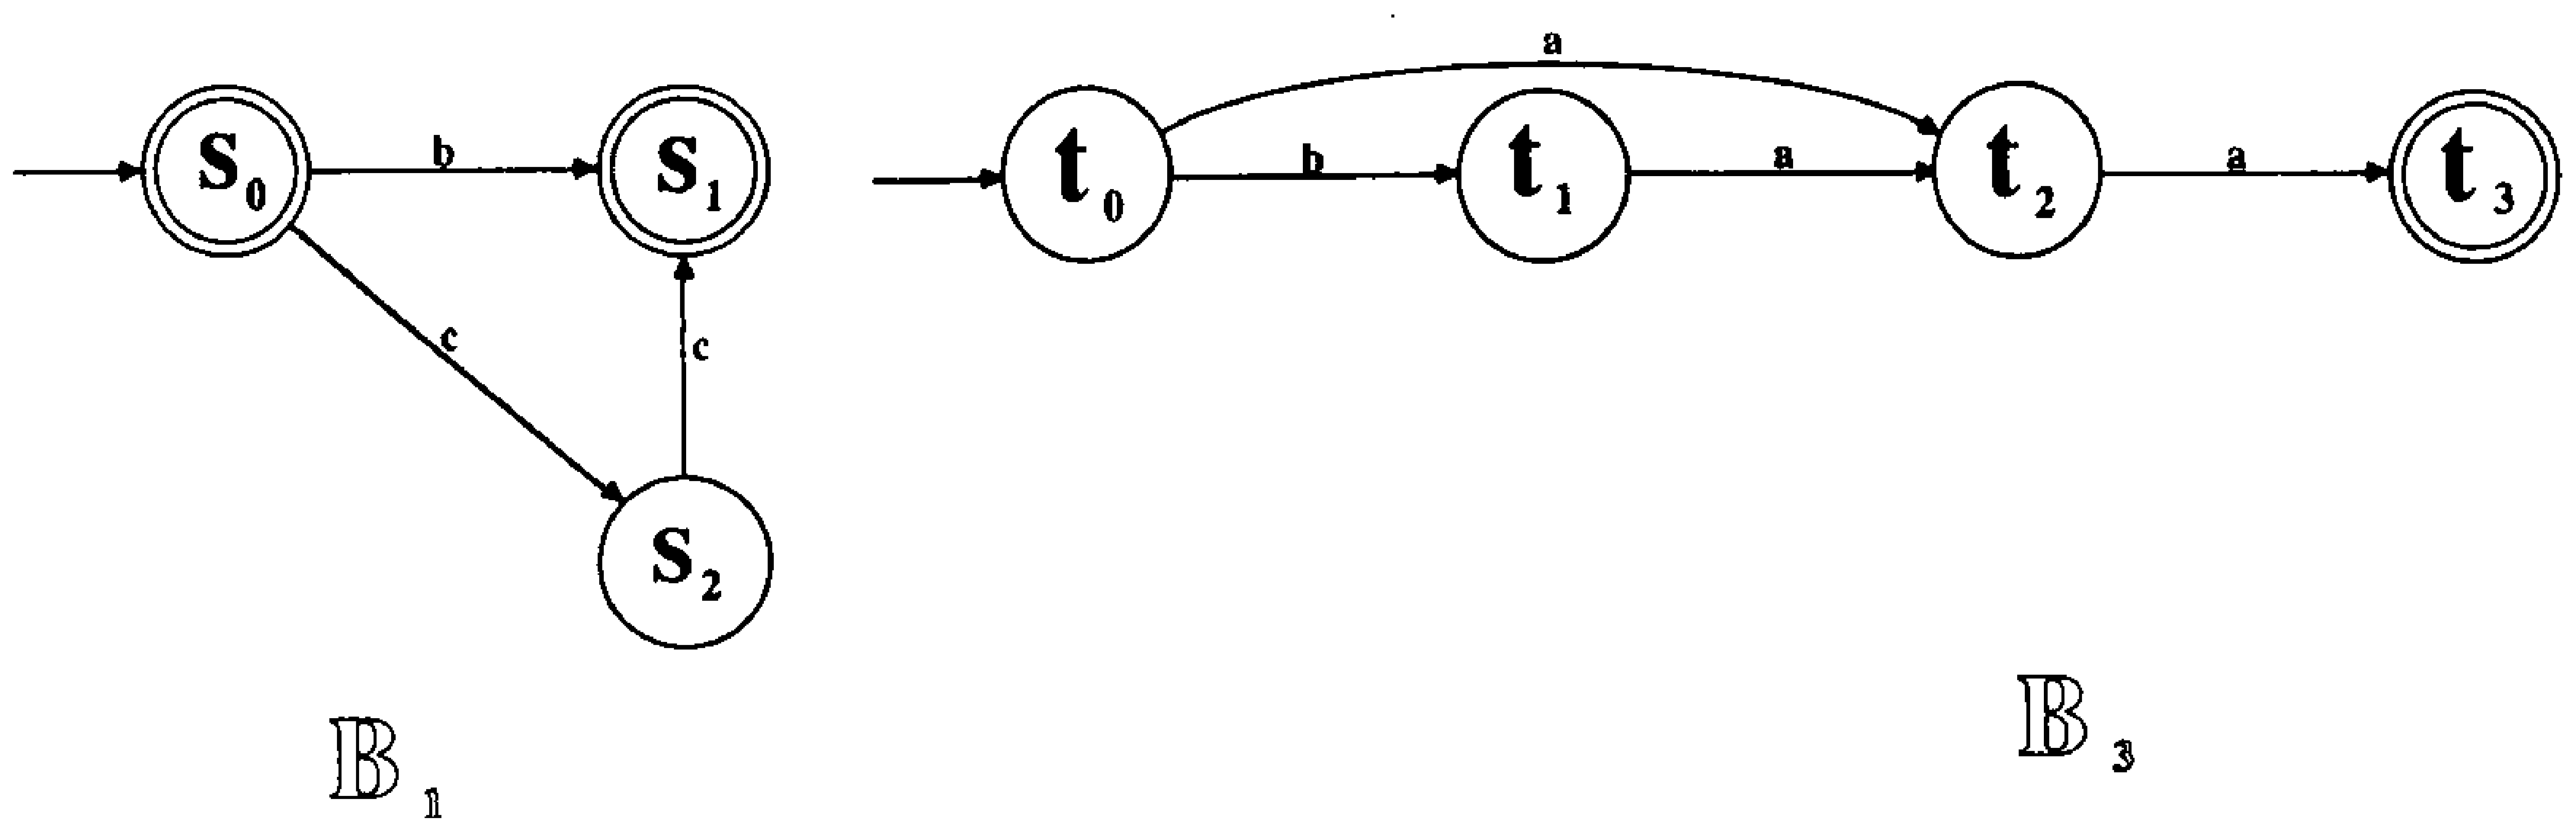
\epsfig{figure=ToFAfigures/fig5-11.eps,width=6in}}
\caption{Candidates for concatenation in which the second machine does not
accept $\lambda$ (Example 5.13)}\label{fig-5.11}
\end{figure}

Besides concatenation, string algebra allows other new operators on languages.
The operators $^*$ and $^+$, which have at this point only been defined for
alphabets, likewise have natural extensions to languages. Loosely, we would
expect $L^*$ to consist of all words that can be formed by the concatenation of
several words from L.
\vspace{1in} % with current spacing, one line of Def5.5 is on page 152,
% followed by two figures at the top of 153, then the rest of Def5.5.  Ugh...

% Figure 5.12
\begin{figure}
\centerline{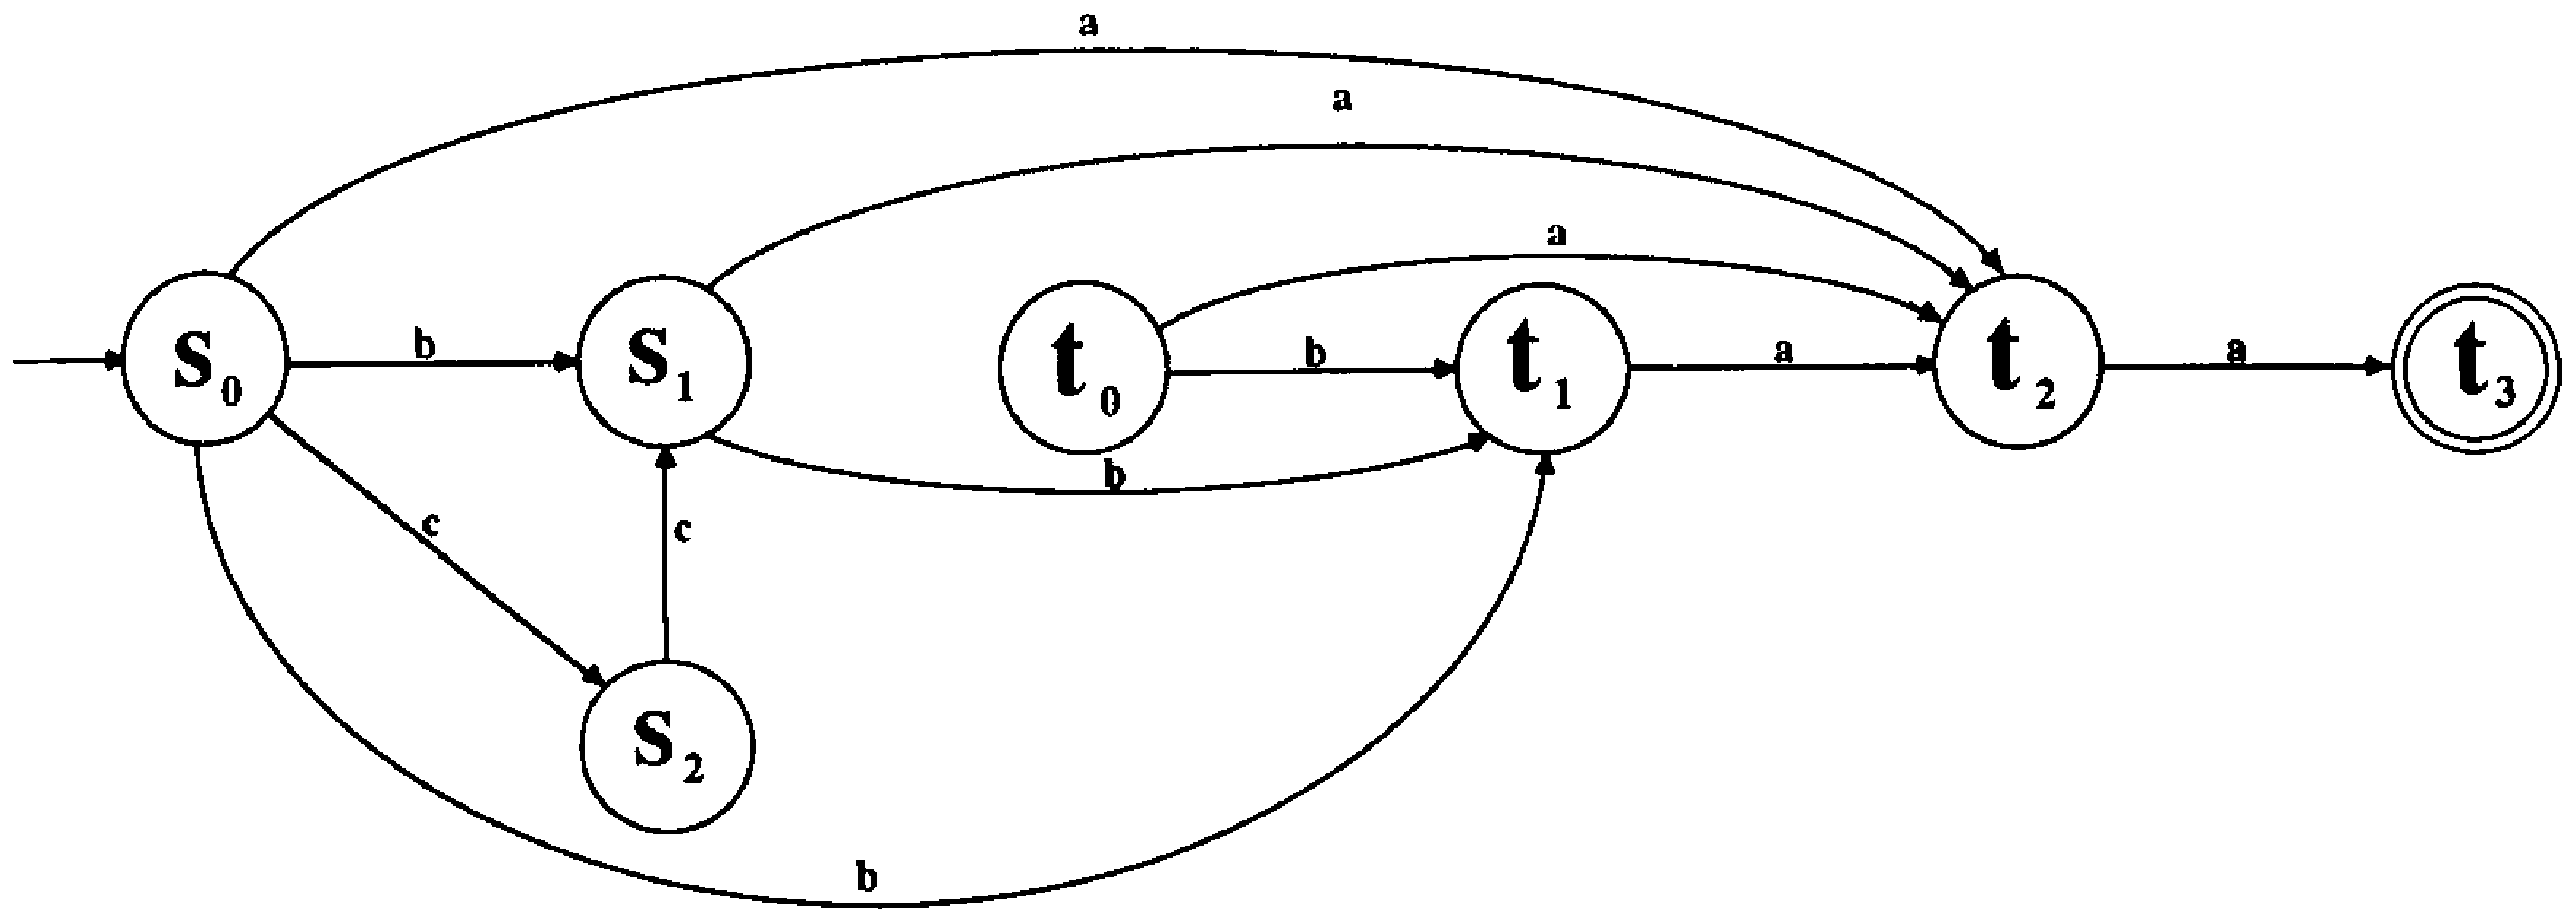
\epsfig{figure=ToFAfigures/fig5-12.eps,width=6in}}
\caption{The concatenation of the NDFAs in Example 5.13}\label{fig-5.12}
\end{figure}

% Definition 5.5
\begin{dfn}\label{dfn-5.5}
Let $L$ be a language over some alphabet $\Sigma$. Define
\begin{center}
\begin{tabular}{l}
$L^0 =\{\lambda\}$ \\
$L^1 = L$ \\
$L^2 = L \cdot L$ \\
$L^3 = L \cdot L^2 = L \cdot L \cdot L$
\end{tabular}
\end{center}
and in general
\begin{center}
\begin{tabular}{l}
$L^n = L\cdot L^{n-1},\qquad \text{for }n = 1,2,3, \ldots$ \\
$L^*= \bigcup\limits^\infty_{i=0} L^i = L^0 \cup L^1 \cup L^2 \cup \cdots =
	\{\lambda\}\cup L\cup L\cdot L\cup L\cdot L\cdot L\cup \ldots$ \\
$L^+= \bigcup\limits^\infty_{i=1} L^i=L^1 \cup L^2 \cup L^3 \cup \cdots =
	L \cup L \cdot L \cup L \cdot L \cdot L \cup \ldots$ \\
\end{tabular}
\end{center}
$L^*$ is called the \emph{\Index{Kleene closure}} of the language $L$.
\end{dfn}

\subsection*{Example 5.14}

If $L =\{\pmb{aa},\pmb{c}\}$, then $L^*=\{\lambda,\pmb{aa},\pmb{c},\pmb{aac},
\pmb{caa},\pmb{aaaa},\pmb{cc},\pmb{aaaaaa},\pmb{aaaac},\pmb{aacaa}, \ldots\}$.

\subsection*{Example 5.15}

If $K =\{\pmb{db},\pmb{b},\pmb{c}\}$, then $K^*$ consists of all words (over
$\{\pmb{b},\pmb{c},\pmb{d}\}$ for which each occurrence of $\pmb{d}$ is immediately followed by (at
least) one $\pmb{b}$.

$\DSIG$ is closed under both $^*$ and $^+$. The technique for
Kleene closure is outlined in Theorem \ref{thm-5.5}. The construction for $L^+$ is similar
(see the exercises).

% Theorem 5.5
\begin{thm}\label{thm-5.5}\index{closure!under Kleene closure}
For any alphabet $\Sigma$, $\DSIG$ is closed under $^*$ (Kleene
closure).

\emph{Proof.} Let L belong to $\DSIG$. Then there is a \underline{non}deterministic
finite automaton $A =\langle\Sigma,S,S_0,\delta,F\rangle$ such that $L(A)=L$.
Define a \underline{non}deterministic machine
$A_*=\langle\Sigma,S_{*},S_{0*},\delta_{*},F_{*}\rangle$,
where
\begin{center}
\begin{tabular}{rll}
$S_{*}=$ & \!\!\!\!$S \cup \{q_0\}\quad \text{(where $q_0$ is some new
	state; $q_0 \notin S$)}$ \\
$S_{0*}=$ &\!\!\!\!$S_0 \cup \{q_0\}$ \\
$F_{*}=$ &\!\!\!\!$F \cup \{q_0\}$
\end{tabular}
\end{center}
and $\delta_{*}$$: (S \cup \{q_0\}) \times \Sigma \rightarrow
	\wp(S \cup \{q_0\})$ is defined by
\[ \delta_{*}(s,\pmb{a}) = \left\{\begin{array}{ll}
		\delta(s,\pmb{a}) & \text{if }s \notin F \cup \{q_0\} \\
		\delta(s,\pmb{a})\cup\left(\bigcup\limits_{t\in S_0}\delta(t,\pmb{a})\right)
			& \text{if }s \in F \\
		\emptyset & \text{if }s = q_0
		\end{array}\right. \]
We claim that $L(A_{*}) = L(A)^* = L^*$ (see the exercises).
\end{thm}

\subsection*{Example 5.16}

Consider the \emph{non}deterministic finite automaton $B$ displayed in Figure 
\ref{fig-5.13}, which accepts all words that contain exactly two (consecutive) $\pmb{b}$s.
Using the modifications described above, the new NDFA $B_{*}$ would look
like the automaton shown in Figure \ref{fig-5.14}. Notice that the new automaton does
indeed accept $L(B)^*$, the set of all words in which the $\pmb{b}$s always occur
in side-by-side pairs. This example also demonstrates the need for the special
extra start (and final) state $q_0$ (see the exercises).

% Figure 5.13
\begin{figure}
\centerline{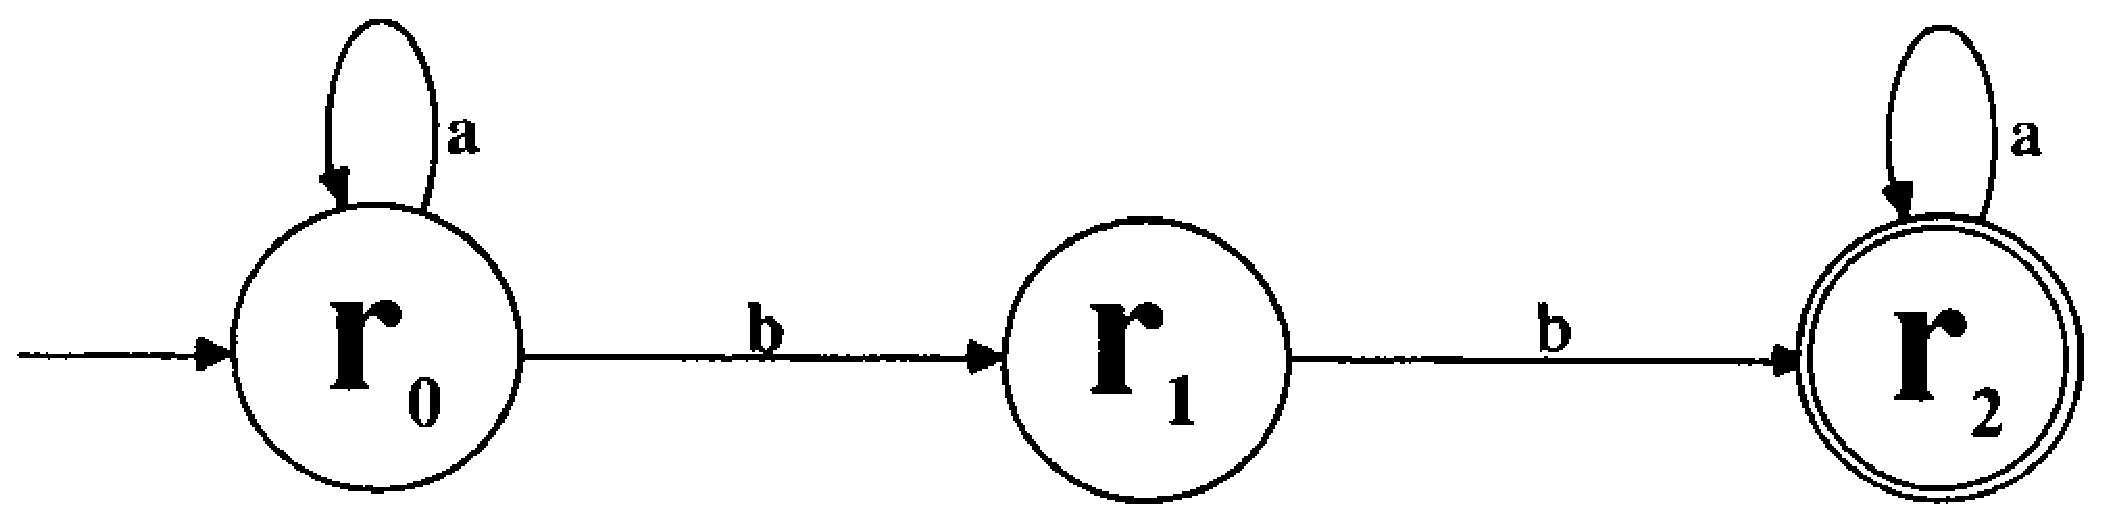
\epsfig{figure=ToFAfigures/fig5-13.eps,width=4in}}
\caption{The NDFA $B$ in Example 5.16.}\label{fig-5.13}
\end{figure}

% Figure 5.14
\begin{figure}
\centerline{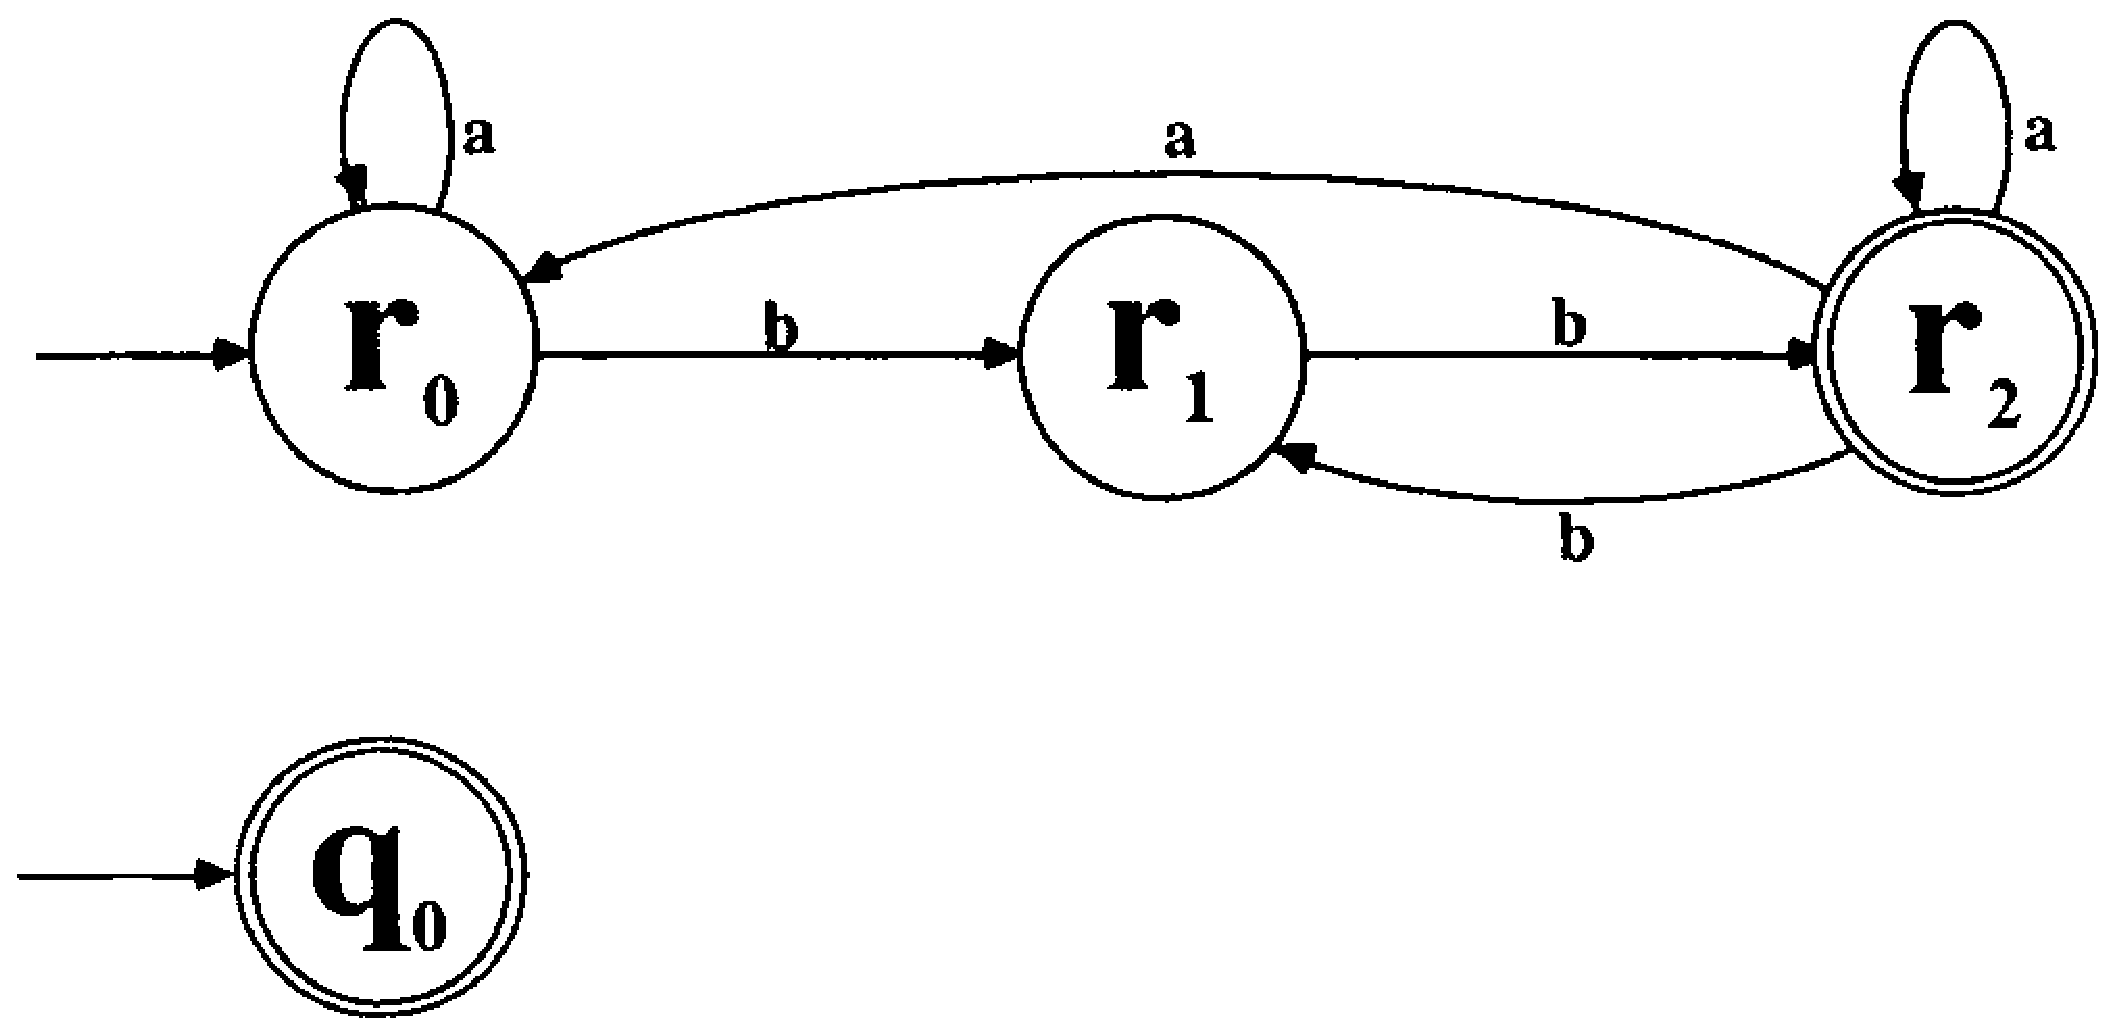
\epsfig{figure=ToFAfigures/fig5-14.eps,width=4in}}
\caption{The resulting NDFA for Example 5.16}\label{fig-5.14}
\end{figure}

It is instructive to compare the different approaches taken in the proofs of
Theorems \ref{thm-5.4} and \ref{thm-5.5}. In both cases, nondeterministic automata were built, but
Theorem \ref{thm-5.4} began with deterministic machines, while Theorem \ref{thm-5.5} assumed that
an NDFA was provided. Note that, in the construction of $\delta^\bullet$ in
Theorem \ref{thm-5.4}, $\delta_1$ was a deterministic transition function and as such
produced a single state, whereas $\delta^\bullet$, on the other hand, must
adhere to the nondeterministic definition and produce a \emph{set} of states. As a
consequence, the definition of $\delta^\bullet$ involved expressions like
$\{\delta_1(s,\pmb{a})\}$, which indicated that the single state given by
$\delta_1(s,\pmb{a})$ should be viewed as a singleton set.

By contrast, Theorem \ref{thm-5.5} specified the nondeterministic transition function
$\delta_{*}$ in terms of $\delta$, which was also assumed to be
nondeterministic. This gave rise to definitions of the form
$\delta_*(s,\pmb{a}) = \delta(s,\pmb{a})$. In this case, no set brackets $\{\ \}$
were necessary since $\delta(s,\pmb{a})$ by assumption already represented a set
(rather than just a single element as in the deterministic case).

The definition of the new set of start states $S_0$ is also affected by the type
of machine from which the new NDFA is formed. In reviewing Theorems \ref{thm-5.4} and \ref{thm-5.5},
the reader should be able to see the parallel between the differences in the
specifications of the $\delta$ function and the differences in the definitions
of $S^\bullet_0$ and $S_{0*}$. It is also instructive to compare and contrast
the proof of Theorem \ref{thm-5.2} to those discussed above.

\section{Further Closure Properties}\label{sec-5.2}

The operators discussed in this section, while not as fundamental as those
presented earlier, illustrate some useful techniques for constructing modified
automata. Also explored are techniques that provide existence proofs rather than
constructive proofs.

% Theorem 5.6
\begin{thm}\label{thm-5.6}
For any alphabet $\Sigma$, $\DSIG$ is closed under the operator Z,
where Z is defined by
\[ Z(L) = \{x \ |\  x \text{ is formed by deleting zero or more letters from a
	word in L}\}. \]

\emph{Proof.} See the exercises and the following example.
\end{thm}

\subsection*{Example 5.17}

Consider the deterministic finite automaton $C$ displayed in Figure \ref{fig-5.15}, which
accepts the language $\{\pmb{a}^n\pmb{b}^m\ |\ n \geq 1,m \geq 1\}.\ Z(L(C))$ would then be
\[ \{\pmb{a}^n\pmb{b}^m\ |\ n \geq 0, m \geq 0\} \]
and can be accepted by modifying $C$ so that every transition in the diagram has
a corresponding $\lambda$-move (allowing that particular letter to be skipped),
as shown in Figure \ref{fig-5.16}.

% Figure 5.15
\begin{figure}
\centerline{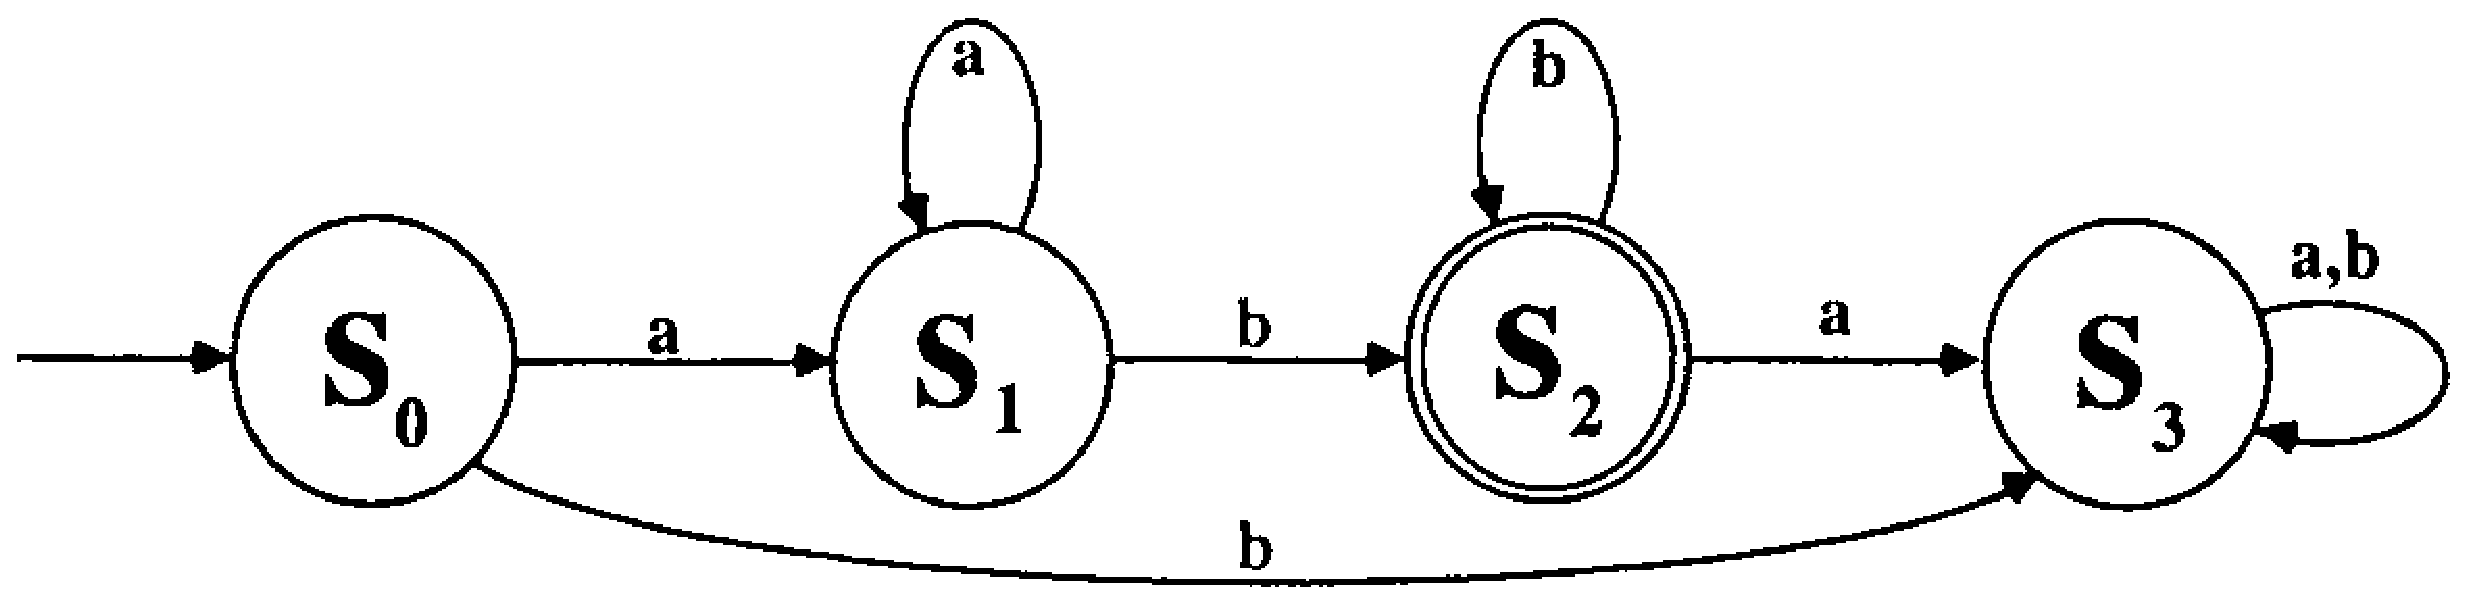
\epsfig{figure=ToFAfigures/fig5-15.eps,width=5in}}
\caption{The automaton $C$ discussed in Example 5.17}\label{fig-5.15}
\end{figure}

% Figure 5.16
\begin{figure}
\centerline{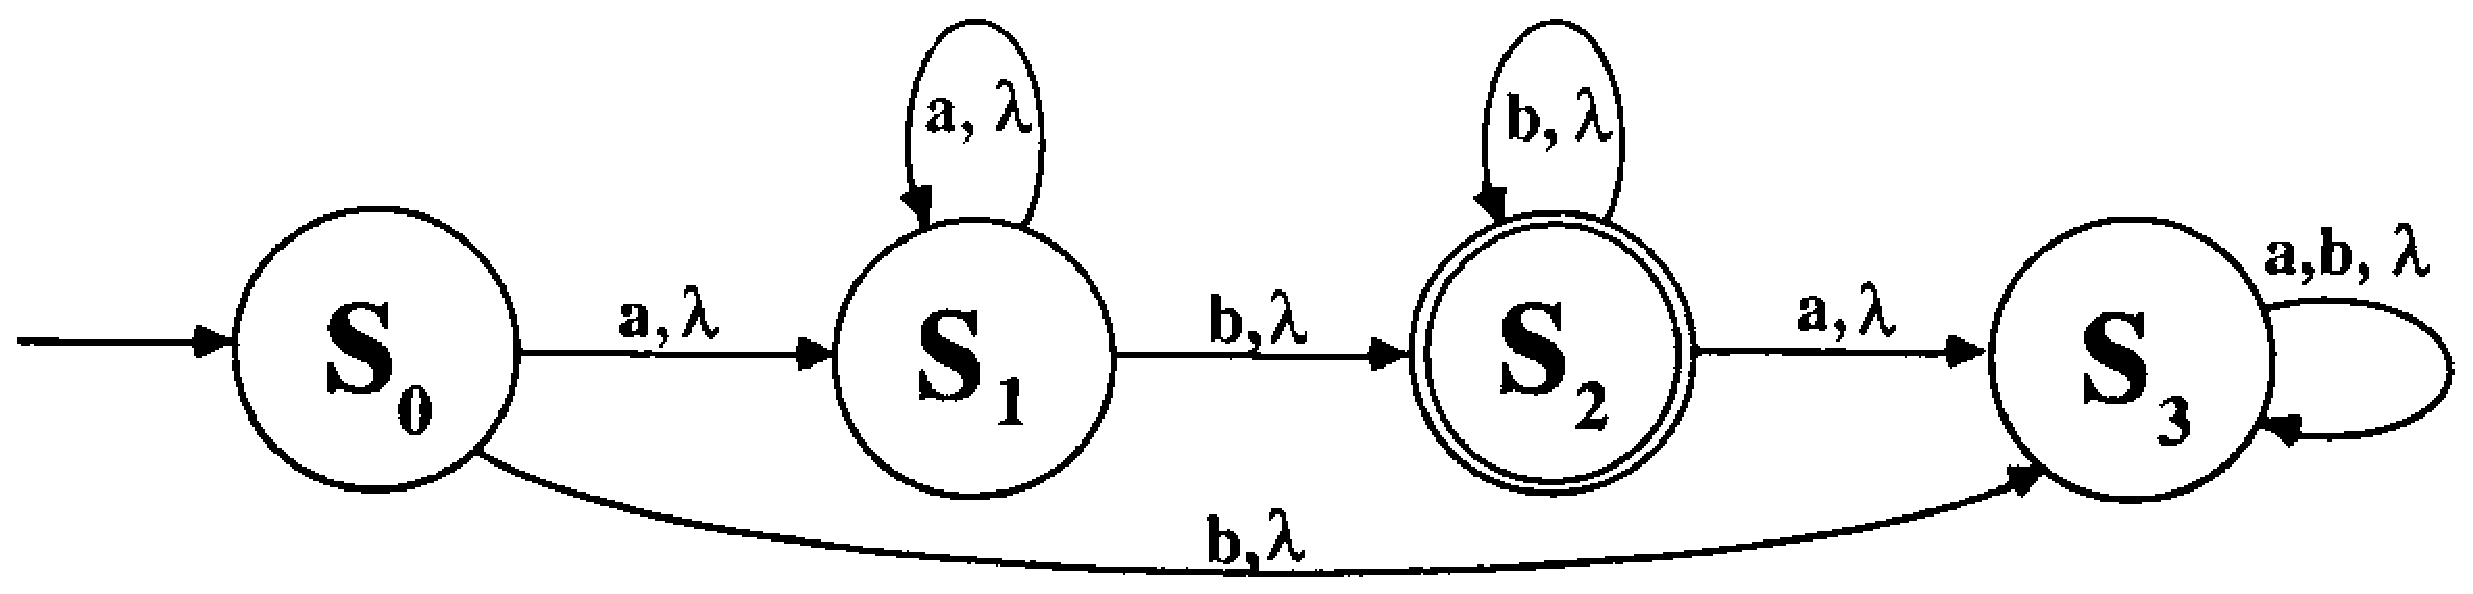
\epsfig{figure=ToFAfigures/fig5-16.eps,width=5in}}
\caption{An automaton accepting $Z(C)$ in Example 5.17}\label{fig-5.16}
\end{figure}

% Figure 5.17
\begin{figure}
\centerline{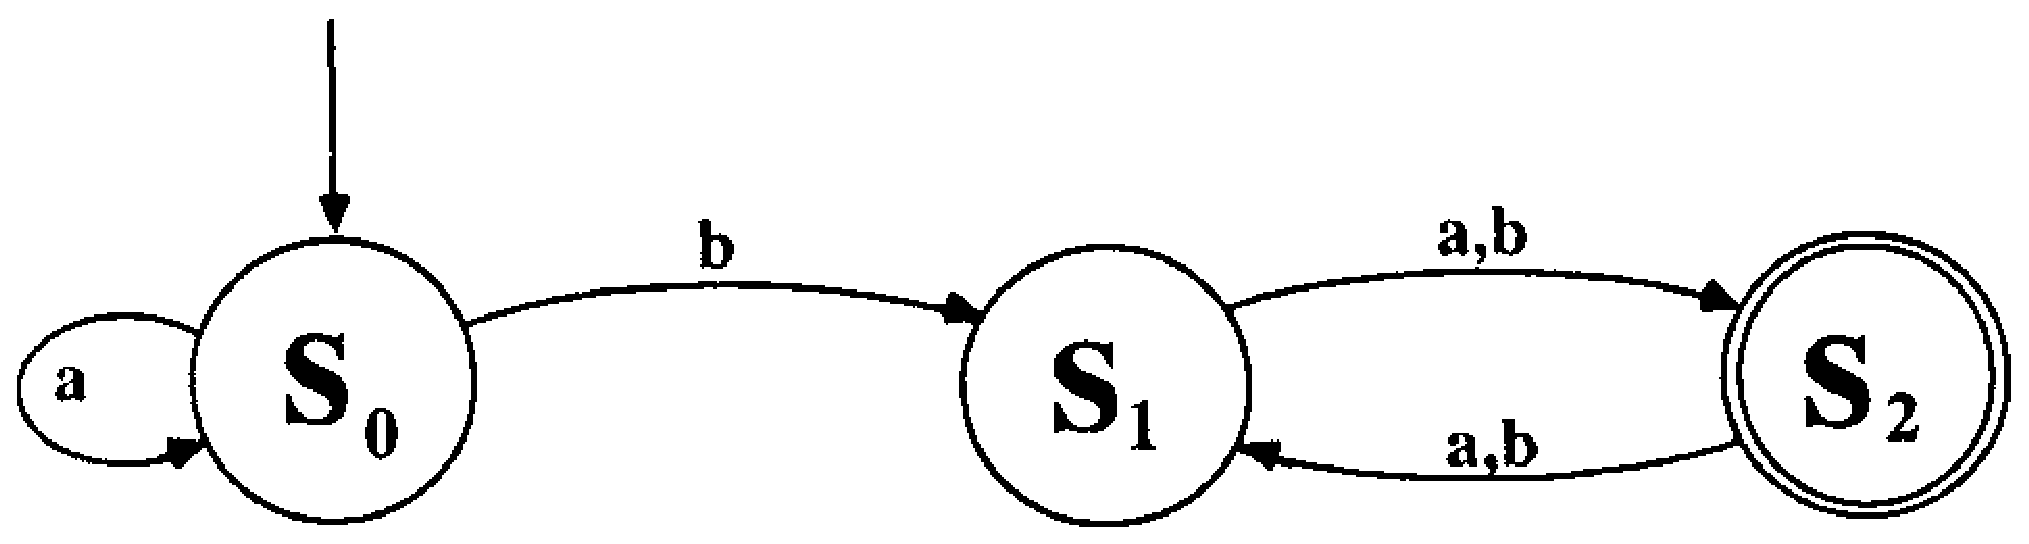
\epsfig{figure=ToFAfigures/fig5-17.eps,width=4in}}
\caption{The automaton $D$ discussed in Example 5.18}\label{fig-5.17}
\end{figure}

% Theorem 5.7
\begin{thm}\label{thm-5.7}
For any alphabet $\Sigma$, $\DSIG$ is closed under the operator
$Y$, where $Y$ is defined by
\[ Y(L) =\{x\ |\ x \text{ is formed by deleting exactly one letter from a
	word in L}\}. \]
\emph{Proof.} See the exercises and the following example.
\end{thm}

\subsection*{Example 5.18}

We need a way to skip a letter as was done in Example 5.17, but we must now
skip one and only one letter. The technique for accomplishing this involves
using \emph{copies} of the original machine. Consider the deterministic finite
automaton $D$ displayed in Figure \ref{fig-5.17}. We will use $\lambda$-moves to mimic
normal transitions, but in this case we will move from one copy of the machine
to an appropriate state in a second copy. Being in the first copy of the machine
will indicate that we have yet to skip a letter, and being in the second copy
will signify that we have followed exactly one $\lambda$-move and have thus
skipped exactly one letter. Hence the second copy will be the only one in which
states are deemed final, and the first copy will contain the only start state.
The modified machine for this example might look like the NDFA shown in Figure
\ref{fig-5.18}. The string $\pmb{aba}$, which is accepted by the original machine, should
cause $\pmb{ab}$, $\pmb{aa}$, and $\pmb{ba}$ to be accepted by the new machine. Each
of these three are indeed accepted, by following the correct $\lambda$-move at
the appropriate time. A similar technique, with the state transition function
slightly redefined, could be used to accept words in which every other letter
was deleted. If one wished only to acknowledge every third letter, three copies
of the machine could be suitably connected together to achieve the desired
result (see the exercises).

% Figure 5.18
\begin{figure}
\centerline{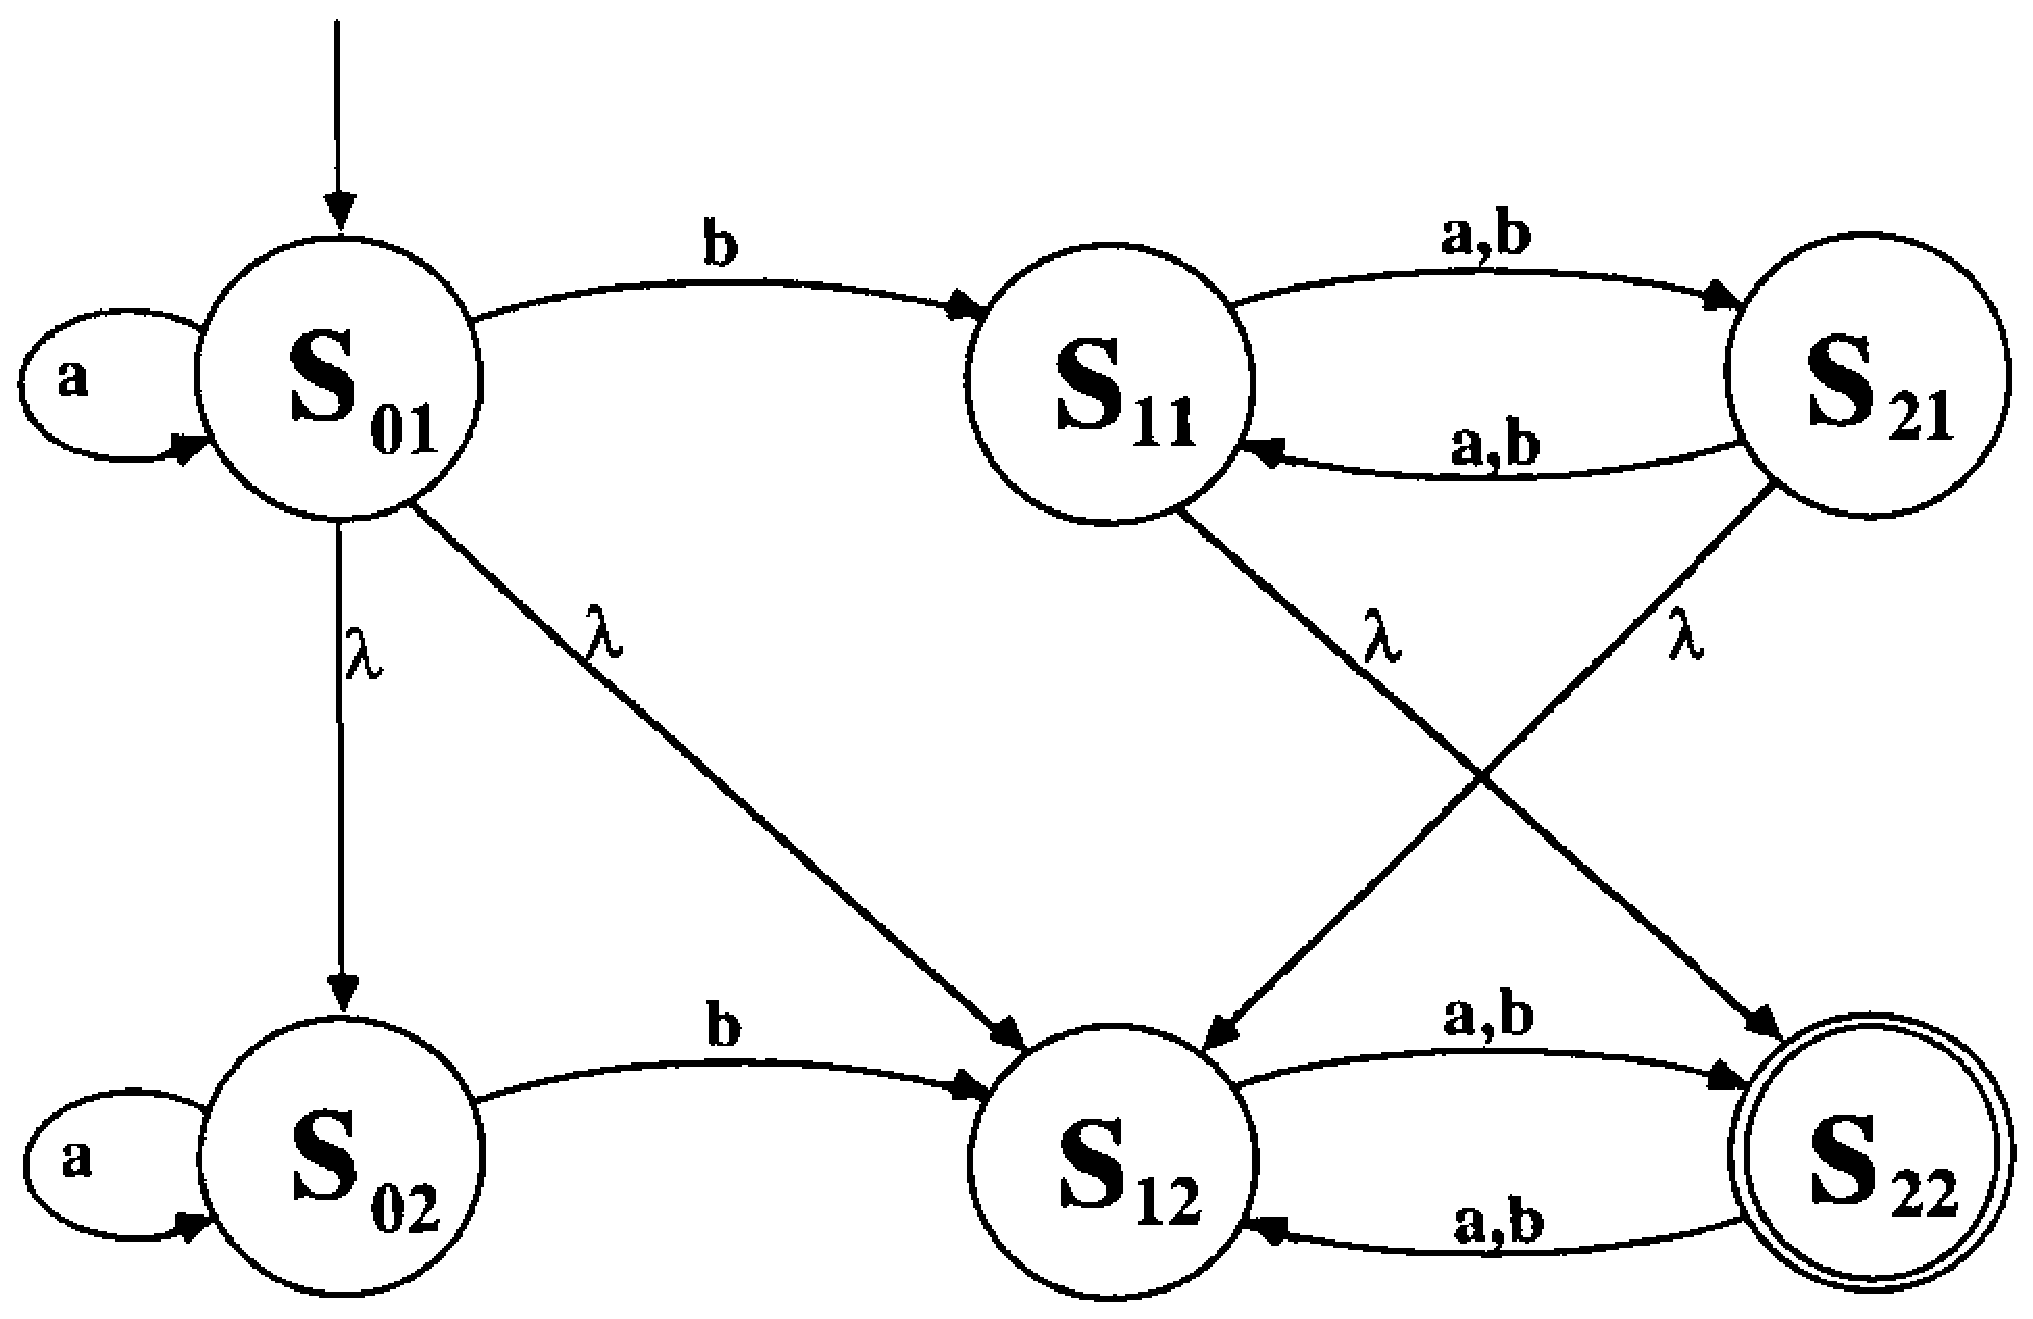
\epsfig{figure=ToFAfigures/fig5-18.eps,width=4in}}
\caption{The modified machine in Example 5.18}\label{fig-5.18}
\end{figure}

While $\DSIG$ is certainly the most important class of languages we have seen so
far, we will now consider some other classes whose properties can be
investigated. The closure properties of other collections of languages will be
considered in the exercises and in later chapters.

% Definition 5.6
\begin{dfn}\label{dfn-5.6}\index{W@\WSIG \ (W-sigma )}
Let $\Sigma$ be an alphabet. Then $\WSIG$ is defined to be the set of all
languages over $\Sigma$ recognized by NDFAs; that is,
\[ \WSIG =\{L \subseteq \Sigma^* \ |\ \exists \text{ NDFA } N \ni L(N)
	= L\}.\]
\end{dfn}

% Lemme 5.2
\begin{lmm}\label{lmm-5.2}
Let $\Sigma$ be an alphabet. Then $\WSIG = \DSIG$.

\emph{Proof.} The proof follows immediately from Theorem \ref{thm-4.1} and Exercise 4.25.
\end{lmm}

The reader should note that Lemma \ref{lmm-5.2} simply restates in new terms the
conclusion reached in Chapter \ref{ch-4}, where it was proved that NDFAs were exactly
as powerful as DFAs. More specifically, it was shown that any language that
could be recognized by an NDFA could also be recognized by a DFA, and conversely.
While every subset of $\Sigma^*$ represents a language, those in \DSIG\ have
exhibited many nice properties owing to the convenient representation afforded
by finite automata. We now focus our attention on ``the other languages,'' that
is, those that are \emph{not} in $\DSIG$.

% Definition 5.7
\begin{dfn}\label{dfn-5.7}\index{N@\NSIG \ (N-sigma )}
Let $\Sigma$ be an alphabet. Then $\NSIG$ is defined to be the set of all
\emph{non}-FAD languages over $\Sigma$; that is,
\[ \NSIG =\{L \subseteq \Sigma^*| \text{ there does \emph{not} exist \emph{any} finite
automaton } M \ni L(M) = L\} \]
\end{dfn}

$\NSIG$ is all the ``complicated'' languages (subsets) that can be formed from
$\Sigma^*$; that is, $\NSIG = \wp(\Sigma^*) - \DSIG$. Be careful not to confuse
\NSIG\ with the set of languages that can be recognized by NDFAs (\WSIG\ in
Definition \ref{dfn-5.6}).

% Theorem 5.8
\begin{thm}\label{thm-5.8}\index{closure!under complementation}
Let $\Sigma$ be an alphabet. Then \NSIG\ is closed under $\sim$ (complementation).

\emph{Proof.} (by contradiction): Assume the lemma is not true, which means that
there exists a language $K$ for which
\begin{center}
\begin{tabular}{rl}
$K \in \NSIG\ \wedge \sim\!\! K \notin \NSIG$ & $\Rightarrow$ (by definition of
	\,\NSIG) \\
$\sim\!\! K \in \DSIG$ & $\Rightarrow$ (by Theorem \ref{thm-5.1}) \\
$\sim\!\!(\sim\!\! K) \in \DSIG$ & $\Rightarrow$ (since
	$\sim\!\!(\sim\!\! K)=K$) \\
$K \in \DSIG$ & $\Rightarrow$ (by definition of \,\NSIG) \\
$K \notin \NSIG$ &
\end{tabular}
\end{center}
which contradicts the assumption. Thus the lemma must be true.
\end{thm}

% Lemma 5.3
\begin{lmm}\label{lmm-5.3}\index{closure!under intersection}
$\mathfrak{N}_{\{\pmb{a},\pmb{b}\}}$ is \emph{not} closed under $\cap$.

\emph{Proof.} Let $L_1=\{\pmb{a}^p\ |\ p$ is prime$\}$ and let $L_2=\{\pmb{b}^p\ |\ p$ is prime$\}$.
Then $L_1 \in \mathfrak{N}_{\{\pmb{a},\pmb{b}\}}$, $L_2 \in \mathfrak{N}_{\{\pmb{a},\pmb{b}\}}$ but
$L_1 \cap L_2 = \emptyset \notin \mathfrak{N}_{\{\pmb{a},\pmb{b}\}}$ (why?).
\end{lmm}

As another useful example of closure, we consider the transformation of one
language to another via a \emph{\Index{language homomorphism}}, which represents
the process of consistently replacing each single letter $\pmb{a}_i$, by a word
$w_i$. Such transformations are commonplace in computer science; some
applications expect lines in a text file to be delimited with a carriage
return/line feed pair, while other applications expect only a carriage return.
Stripping away the unwanted line feeds is tantamount to applying a homomorphism
that replaces most ASCII characters by the same symbol, but replaces line feeds
by $\lambda$. Converting all lowercase letters in a file to uppercase is another
common transformation that can be defined by a language homomorphism.

% Definition 5.8
\begin{dfn}\label{dfn-5.8}
Let $\Sigma=\{\pmb{a_1},\pmb{a_2}, \ldots , \pmb{a_m}\}$ be an alphabet and let
$\Gamma$ be a second alphabet. Given words $w_1,$ $w_2,\ldots ,w_m$ over $\Gamma^*$\!\!,
define a \emph{language homomorphism} $\psi$$: \Sigma \rightarrow \Gamma^*$ by
$\psi(\pmb{a}_i) = w_i$ for each $i$, which can be extended to
$\PBAR$$: \Sigma^* \rightarrow \Gamma^*$ by:
\begin{center}
\begin{tabular}{rcl}
$\PBAR(\lambda)$ & $=$ & $\lambda$ \\
$(\forall \pmb{a} \in \Sigma)(\forall x \in \Sigma^*)(\PBAR(\pmb{a}\cdot x)$ & $=$ &
	$\psi(\pmb{a}) \cdot (\PBAR(x)))$
\end{tabular}
\end{center}
\PBAR can be further extended to operate on a language $L$ by defining
\[ \PBAR(L) =\{\PBAR(z) \in \Gamma^* |\  z \in L\} \]
In this context, $\PBAR$$: \wp(\Sigma^*) \rightarrow \wp(\Gamma^*)$.
\end{dfn}

\subsection*{Example 5.19}

Let $\Sigma =\{\pmb{a},\pmb{b}\}$ and $\Gamma =\{\pmb{c},\pmb{d}\}$, and define
$\psi$ by $\psi(\pmb{a})=\pmb{cd}$ and $\psi(\pmb{b})=\pmb{d}$. For
$K=\{\lambda,\pmb{ab},\pmb{bb}\}$, $\psi(K)=\{\lambda,\pmb{cdd},\pmb{dd}\}$,
while for $L=\{\pmb{a},\pmb{b}\}^*$, $\PBAR(L)$ represents all words over
$\{\pmb{c},\pmb{d}\}$ in which every $\pmb{c}$ is immediately followed by $\pmb{d}$.

\subsection*{Example 5.20}

As a second example, let $\Sigma=\{),(\}$ and let $\Gamma$ be the ASCII
alphabet. If $\mu$ is defined by $\mu(() =$ {\bf begin} and $\mu())=$ {\bf end},
then the set $M$ of all strings of matched parentheses maps to $K$, the set of
all matched {\bf begin}-{\bf end} pairs.

A general homomorphism $\psi$ maps a language over $\Sigma$ to a language over
$\Gamma$. However, to consider the closure of \DSIG, we will restrict our
attention for the moment to homomorphisms for which $\Gamma=\Sigma$. It is more
generally true, though, that even for language homomorphisms between two
different alphabets, if $L$ is FAD, the homomorphic image of L is also FAD (see
the exercises).

% Theorem 5.9
\begin{thm}\label{thm-5.9}\index{closure!under language homomorphism}
Let $\Sigma$ be an alphabet, and let $\psi$$: \Sigma \rightarrow \Sigma^*$ be a
language homomorphism. Then \DSIG\ is closed under $\PBAR$.

\emph{Proof.} See the exercises and the following examples. A much more concise
way to handle this transformation will be seen in Chapter \ref{ch-6} when substitutions
are explored.
\end{thm}

If the homomorphism is \emph{\Index{length preserving}}, that is, if it always
maps letters to single letters, it is relatively easy to define a new automaton
from the old one. Indeed, the state transition diagram hardly changes at all;
all transitions marked $\pmb{b}$ are simply relabeled with the new letter $\psi(\pmb{b})$. For
more complex homomorphisms, extra states must be added to accommodate the
processing of the surplus letters. The following two examples illustrate the
appropriate transformation of the state transition function and suggest a
convenient labeling for the new states.

\subsection*{Example 5.21}

Consider the DFA B displayed in Figure \ref{fig-5.19}a. For the homomorphism $\xi$ defined
by $\xi(\pmb{a})=\pmb{a}$ and $\xi(\pmb{b})=\pmb{a}$, the automaton that will
accept $\overline\xi(L(B))$ is shown in Figure \ref{fig-5.19}b. Note that even in simple examples
like this one the resulting automaton can be nondeterministic.

% Figure 5.19
\begin{figure}
\centerline{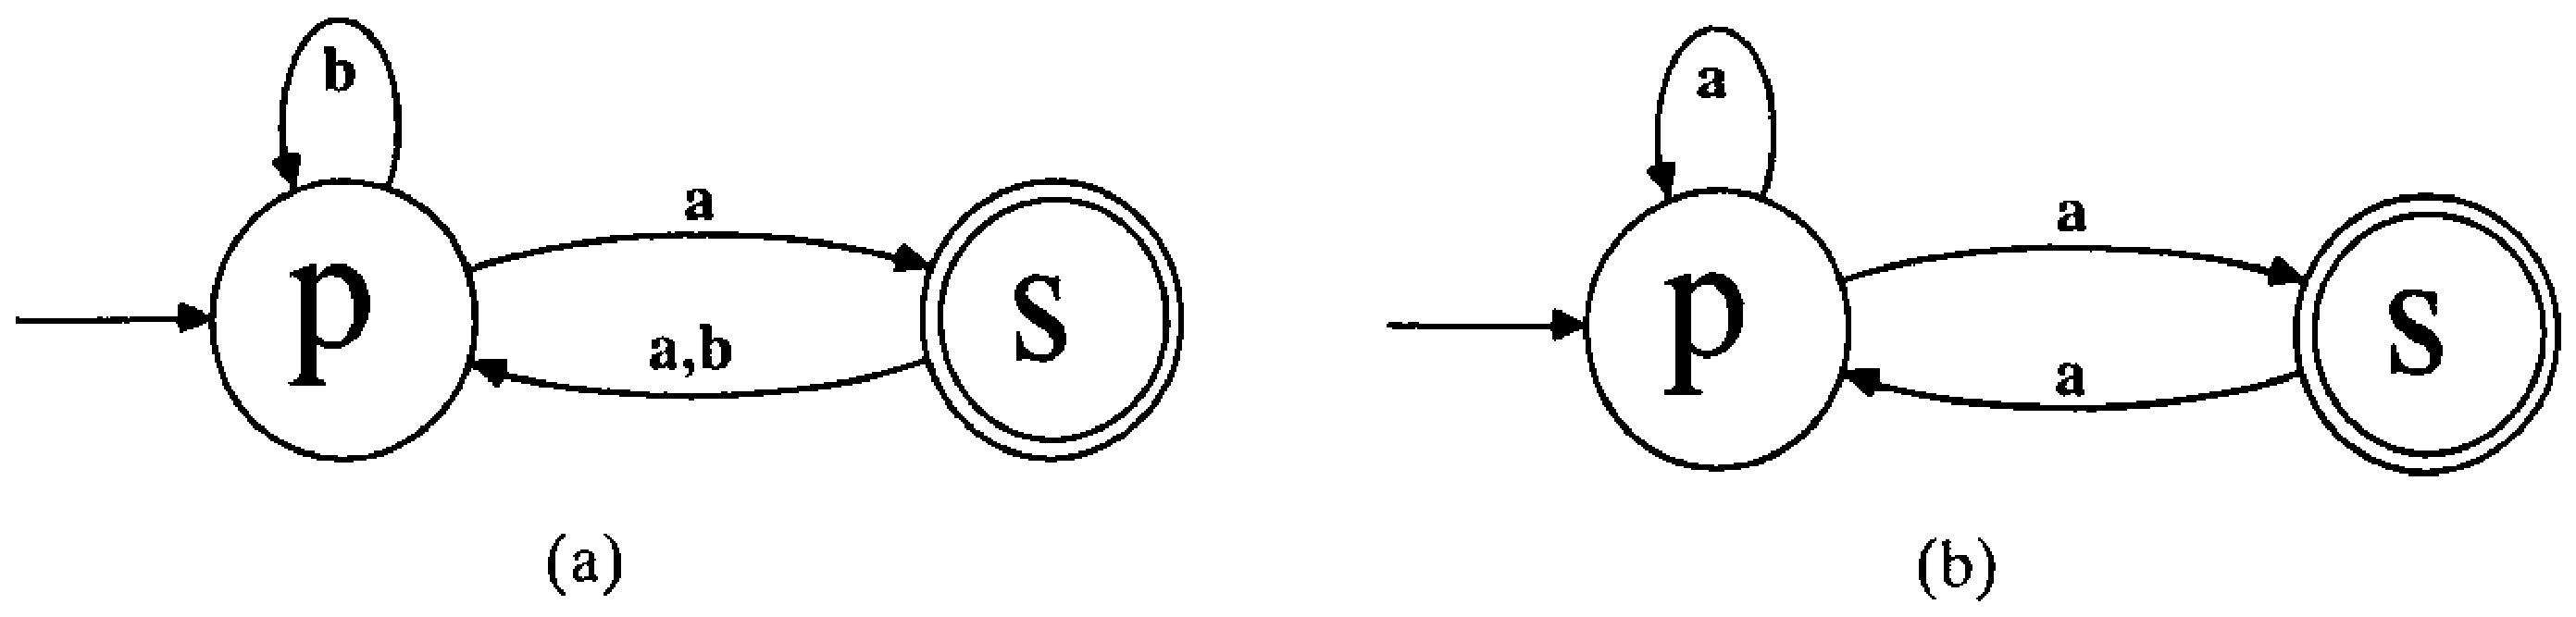
\epsfig{figure=ToFAfigures/fig5-19.eps,width=5.5in}}
\caption{(a) The automaton discussed in Example 5.21; (b) The resulting automaton
for Example 5.21}\label{fig-5.19}
\end{figure}

\subsection*{Example 5.22}

For the NDFA C displayed in Figure \ref{fig-5.20}a and the homomorphism $\mu$ defined by
$\mu(\pmb{a})=\pmb{cc}$ and $\mu(\pmb{b})=\pmb{a}$, the automaton that will
accept $\overline\mu(L(C))$ is shown in Figure \ref{fig-5.20}b. Note that each state of $C$
requires an extra state to accommodate the $\pmb{cc}$ transition.

% Figure 5.20
\begin{figure}
\centerline{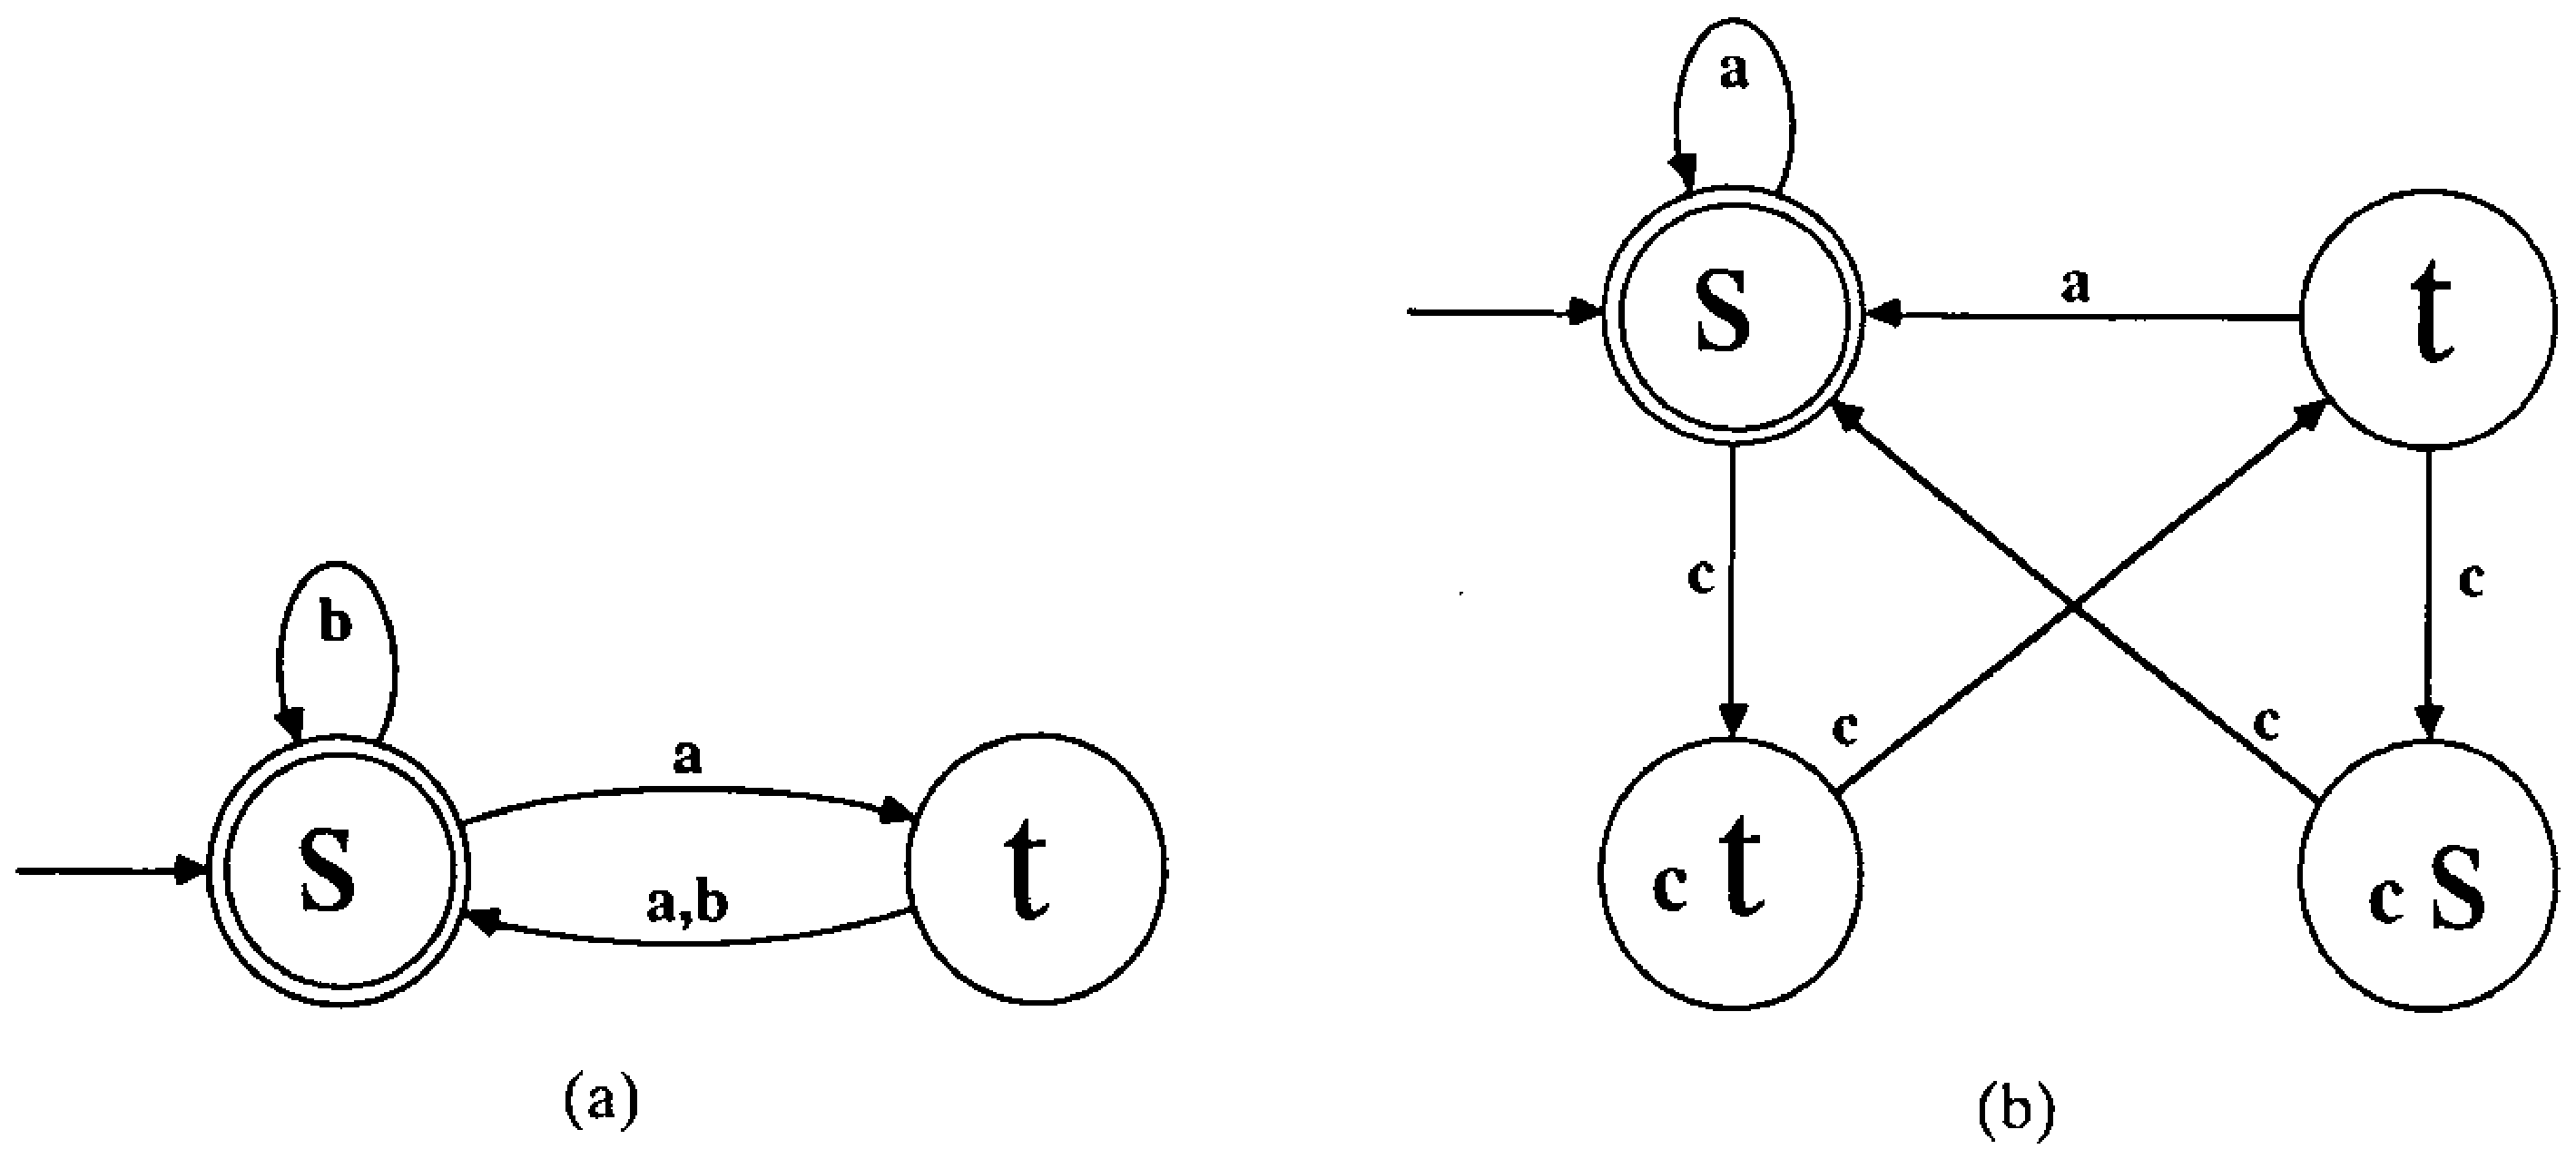
\epsfig{figure=ToFAfigures/fig5-20.eps,width=5.5in}}
\caption{(a) The automaton discussed in Example 5.22; (b) The resulting automaton
for Example 5.22}\label{fig-5.20}
\end{figure}

\subsection*{Example 5.23}

Consider the \emph{identity} homomorphism $\mu$$: \Sigma\rightarrow\Sigma^*$
defined by $(\forall \pmb{a} \in \Sigma)(\mu(\pmb{a})=\pmb{a})$. Since
$\overline{\mu}(L)=L$, \emph{any} collection of languages, including \NSIG, is
clearly closed under this homomorphism. Unlike \DSIG, though, there are many
homomorphisms under which \NSIG\ is not closed.

% Lemma 5.4
\begin{lmm}\label{lmm-5.4}\index{closure!under language homomorphism}
Let $\Sigma=\{\pmb{a},\pmb{b}\}$, and let $\xi$$: \Sigma\rightarrow\Sigma^*$ be
defined by $\xi(\pmb{a})=\pmb{a}$ and $\xi(\pmb{b})=\pmb{a}$. Then \NSIG\ is \emph{not}
closed under $\overline{\xi}$.

\emph{Proof.} Consider the set $L$ of all strings that have the same number of
$\pmb{a}$s as $\pmb{b}$s. This language is in \NSIG, but $\overline{\xi}(L)$ is the
set of all even-length strings of $\pmb{a}$s, which is clearly not in \NSIG.
\end{lmm}

A rather trivial example involves the homomorphism defined by $\psi(a)=\lambda$
for every letter $\pmb{a} \in \Sigma$. Then for all languages $L$, whether or
not $L \in \NSIG,\ \PBAR(L)=\{\lambda\}$, which is definitely not in \NSIG.

% Definition 5.9
\begin{dfn}\label{dfn-5.9}
Let $\psi$$: \Sigma\rightarrow\Gamma^*$ be a language homomorphism and consider
$z \in\Gamma^*$, The \emph{\Index{inverse homomorphic image} of z under $\PBAR$}
is then
\[ \overline{\psi^{-1}}(z)=\{x \in \Sigma^*\ |\ \PBAR(x) = z\} \]
For a language $L \subseteq \Gamma^*$, the \emph{\Index{inverse homomorphic
image} of L under} $\PBAR$ is defined by
\[ \overline{\psi^{-1}}(L)=\{x \in \Sigma^*\ |\ \PBAR(x) \in L\} \]
\end{dfn}

Thus, $x \in \overline{\psi^{-1}}(L) \Leftrightarrow \PBAR(x) \in L$. While the image of a
string under a homomorphism is a single word, note that the inverse image of a
single string may be an entire set of words.

\subsection*{Example 5.24}

Consider $\overline{\xi}$ from Lemma \ref{lmm-5.4} in which $\xi$$: \Sigma \rightarrow
\Sigma^*$ was defined by $\xi(\pmb{a})=\pmb{a}$ and $\xi(\pmb{b})=\pmb{a}$. Let
$z=\pmb{aa}$. Since $\overline{\xi}(\pmb{bb})=\overline{\xi}(\pmb{ba}) =
\overline{\xi}(\pmb{ab})=\overline{\xi}(\pmb{aa})=\pmb{aa}$,
\[ \overline{\xi^{-1}}\!(\pmb{aa})=\{\pmb{bb},\pmb{ba},\pmb{ab},\pmb{aa}\}
\text{. Note that } \overline{\xi^{-1}}\!(\pmb{ba})=\emptyset. \]

For $L=\{x \in\{\pmb{a}\}^*|\ |x|\equiv 0\bmod{3}\},\ 
\overline{\xi^{-1}}\!(L)=\{x\in\{\pmb{a},\pmb{b}\}^*|\ |x|\equiv 0\bmod{3}\}$.
Note that this second set is definitely larger, since it also contains words
with $\pmb{b}$s in them.

It can be shown that \DSIG\ is closed under inverse homomorphism. The trick is to
make the state transition function of the new automaton \emph{simulate}, for a
given letter $\pmb{a}$, the action the old automaton would have taken for the
entire string $\psi(\pmb{a})$. As the following proof will illustrate, the only
change that need take place is in the $\delta$ function; the newly constructed
machine is even deterministic!

% Theorem 5.10
\begin{thm}\label{thm-5.10}\index{closure!under inverse homomorphism}
Let $\Sigma$ be an alphabet, and let $\psi$$: \Sigma \rightarrow \Sigma^*$ be a
language homomorphism. Then \DSIG\ is closed under $\overline{\psi^{-1}}$.

\emph{Proof.} Let $L \in \DSIG$. Then there exists a DFA
$A=\langle\Sigma,S,s_0,\delta,F\rangle$ such that $L(A)=L$. Define a new DFA
$A^\psi=\langle\Sigma,S^\psi,s_0^\psi,\delta^\psi,F^\psi\rangle$ by
\begin{center}
\begin{tabular}{c}
$S^\psi = S$ \\
$s_0^\psi = s_0$ \\
$F^\psi = F$
\end{tabular}
\end{center}
and $\delta^\psi$ is defined by
\[ \delta^\psi(s,\pmb{a})=\DBAR\!(s,\psi(\pmb{a}))\ 
		\forall s \in S, \forall \pmb{a} \in \Sigma \]
Induction can be used to show $\overline{\delta^\psi}\!\!(s,x)=\DBAR(s,\PBAR(x))\forall s \in S,
\forall x \in \Sigma^*$\!\!, and in particular $\overline{\delta^{\psi}}(s_0,x)=\DBAR(s_0,\PBAR(x))$
$\forall x \in \Sigma^*$\!\!. Hence $L(A^\psi)=\overline{\psi^{-1}}(L(A))$.
\end{thm}

This theorem makes it possible to extend the range of the pumping lemma (Theorem
\ref{thm-2.3}) to many otherwise unpleasant problems. The set $M$ given in Example 5.20
can easily be shown to violate Theorem \ref{thm-2.3} and is therefore not FAD. The set $K$
given in Example 5.20 is just as clearly not FAD, but this is quite tedious to
formally prove by the pumping lemma (the number of choices for $u$, $v$, and $w$
is prohibitively large to thoroughly cover). An argument might proceed as
follows: Assume $K$ were FAD. Then $M$, being the inverse homomorphic image of a
FAD language, must also be FAD. Since $M$ is known (by an easy pumping lemma
proof) to be definitely not FAD, the assumption that $K$ is FAD must be
incorrect. Thus, $K \in \NSIG$.

% Lemma 5.5
\begin{lmm}\label{lmm-5.5}\index{closure!under inverse homomorphism}
Let $\Sigma=\{\pmb{a},\pmb{b}\}$, and let $\xi$$: \Sigma\rightarrow\Sigma^*$ be
defined by $\xi(\pmb{a})=\pmb{a}$ and $\xi(\pmb{b})=\pmb{a}$. Then \NSIG\ is
\emph{not} closed under $\overline{\xi^{-1}}$.

\emph{Proof.} Consider the set $L$ of all strings that have the same number of
$\pmb{a}$s as $\pmb{b}$s. This language is in \NSIG\ but $\overline{\xi^{-1}}(L)$ is
$\{\lambda\}$, which is clearly not in \NSIG.
\end{lmm}

We close this chapter by considering two operators for which it is definitely
not convenient to modify the structure of an existing automaton to construct a
new automaton with which to demonstrate closure.

% Theorem 5.11
\begin{thm}\label{thm-5.11}
Let $\Sigma$ be an alphabet. Define the operator $b$ by
\[ L^b=\{x\ |\ \exists y \in \Sigma^* \ni (xy \in L \wedge |x| = |y|)\} \]
Then \DSIG\ is closed under the operator $b$.

\emph{Proof.} $L^b$ represents the first halves of all the words in $L$. For
example, if $K=\{\pmb{ad},\pmb{abaa},\pmb{ccccc}\}$, then
$K^b=\{\pmb{a},\pmb{ab}\}$. Assume that $L$ is FAD. Then there exists a DFA 
$A=\langle\Sigma,S,s_0,\delta,F\rangle$ that accepts $L$. The proof consists of
identifying those states $q$ that are ``midway'' between the start state and a
final state; specifically, we need to identify the set of \emph{strings} for
which $q$ is the midpoint. The previous closure results for union, intersection,
homomorphism, and inverse homomorphism will be used to construct the language
representing $L^b$. Define the \emph{\Index{length}} homomorphism
$\psi$$: \Sigma\rightarrow\{\pmb{1}\}^*$ by $\psi(\pmb{a})=\pmb{1}$ for all
$\pmb{a} \in \Sigma$. Note that $\PBAR$ effectively counts the number of letters in a
word:
\[ \PBAR(x) = \pmb{1}^{|x|} \]
The following argument can be applied to each state $q$ to determine the set of
strings that use it as a ``midway'' state.

Consider the initial set for $q$, $I(A,q)=\{x\ |\ \DBAR(s_0,x)=q\}$ and the
terminal set for $q$, $T(A,q)=\{x\ |\ \DBAR(q,x) \in F\}$. We are interested in
finding those words in $I(A,q)$ that are the same length as words in $T(A,q)$.
$\PBAR(I(A,q))$ represents strings of $\pmb{1}$s whose lengths are the same as
words in $I(A,q)$. A similar interpretation can be given for $\PBAR(T(A,q))$.
Therefore, $\PBAR(I(A,q)) \cap \PBAR(T(A,q))$ will reflect those lengths that
are common to both the initial set and the terminal set. The inverse image under
\PBAR\ for this set will then reflect only those strings in $\Sigma^*$ that are
of the correct length to reach $q$ from $s_0$. This set is
$\overline{\psi^{-1}}(\PBAR(I(A,q)) \cap \PBAR(T(A,q)))$. Not all strings of a given
length are likely to reach $q$, though, so this set must be intersected with
$I(A,q)$ to correctly describe those strings that are both of the proper length
and that reach $q$ from the start state. This set,
$I(A,q) \cap \overline{\psi^{-1}}(\PBAR(I(A,q)) \cap \PBAR(T(A,q)))$, is thus the first
halves of all words that have $q$ as their midpoint. This process can be
repeated for each of the (finite) number of states in the automaton $A$, and the
union of the resulting sets will form all the first halves of words that are
accepted by $A$; that is, the union will equal $L^b$.

Note that by moving the start state of $A$ and forming the automaton
$A^q=\langle\Sigma,S,q,\delta,F\rangle$, each of the initial sets $I(A,q)$ can
be shown to be FAD. Similarly, the automaton
$A_q=\langle\Sigma,S,s_0,\delta,\{q\}\rangle$ illustrates that each terminal set
$T(A,q)$ must be FAD, also. Since $L^b$ has now been shown to be formed from
these basic FAD sets by applying homomorphisms, intersections, inverse
homomorphisms, and unions, $L^b$ must be FAD since \DSIG\ is closed under each
of these types of operations.
\end{thm}

\subsection*{Example 5.25}

Consider the automaton $A$ displayed in Figure \ref{fig-5.21}. For the state highlighted
as $q$, the quantities discussed in Theorem \ref{thm-5.11} would be as follows:
\begin{center}
\begin{tabular}{rcl}
$I(A,q)$ & $=$ & $\{\pmb{abc},\pmb{abcabc},\pmb{abcabcabc},\pmb{abcabcabcabc},
	\ldots\}$ \\
$T(A,q)$ & $=$ & $\{\pmb{aa},\pmb{aaaa},\pmb{aaaaaa},\pmb{aaaaaaaa},\ldots\}$ \\
& $=$ & $\{\pmb{a}^2,\pmb{a}^4,\pmb{a}^6,\pmb{a}^8,\pmb{a}^{10},\pmb{a}^{12},
	\ldots\}$ \\
$\PBAR(I(A,q))$ & $=$ & $\{\pmb{1}^3,\pmb{1}^6,\pmb{1}^9,\pmb{1}^{12},
	\pmb{1}^{15}, \ldots \}$ \\
$\PBAR(T(A,q))$ & $=$ & $\{\pmb{1}^2, \pmb{1}^4,\pmb{1}^6,\pmb{1}^8,\pmb{1}^{10},
	\pmb{1}^{12}, \ldots \}$ \\
$\PBAR(I(A,q))\cap\PBAR(T(A,q))$ & $=$ & $\{\pmb{1}^6,\pmb{1}^{12},\pmb{1}^{18},
	\ldots\}=\{x\in\{\pmb{1}\}^+|\ \ |x|\equiv 0\bmod{6}\}$ \\
$\overline{\psi^{-1}}(\PBAR(I(A,q))\cap\PBAR(T(A,q)))$ & $=$ & $\{x\in\{\pmb{a},\pmb{b},
	\pmb{c}\}^+|\ \ |x| \equiv 0\bmod{6}\}$ \\
& $=$ & $\{\pmb{aaaaaa},\pmb{aaaaab},\pmb{aaaaac},\pmb{aaaaba},\pmb{aaaabb},
	\ldots \}$ \\
$I(A,q)\cap\overline{\psi^{-1}}(\PBAR(I(A,q))\cap\PBAR(T(A,q)))$ & $=$ & $\{\pmb{abcabc},
	\pmb{abcabcabcabc}, \ldots \}$
\end{tabular}
\end{center}

% Figure 5.21
\begin{figure}
\centerline{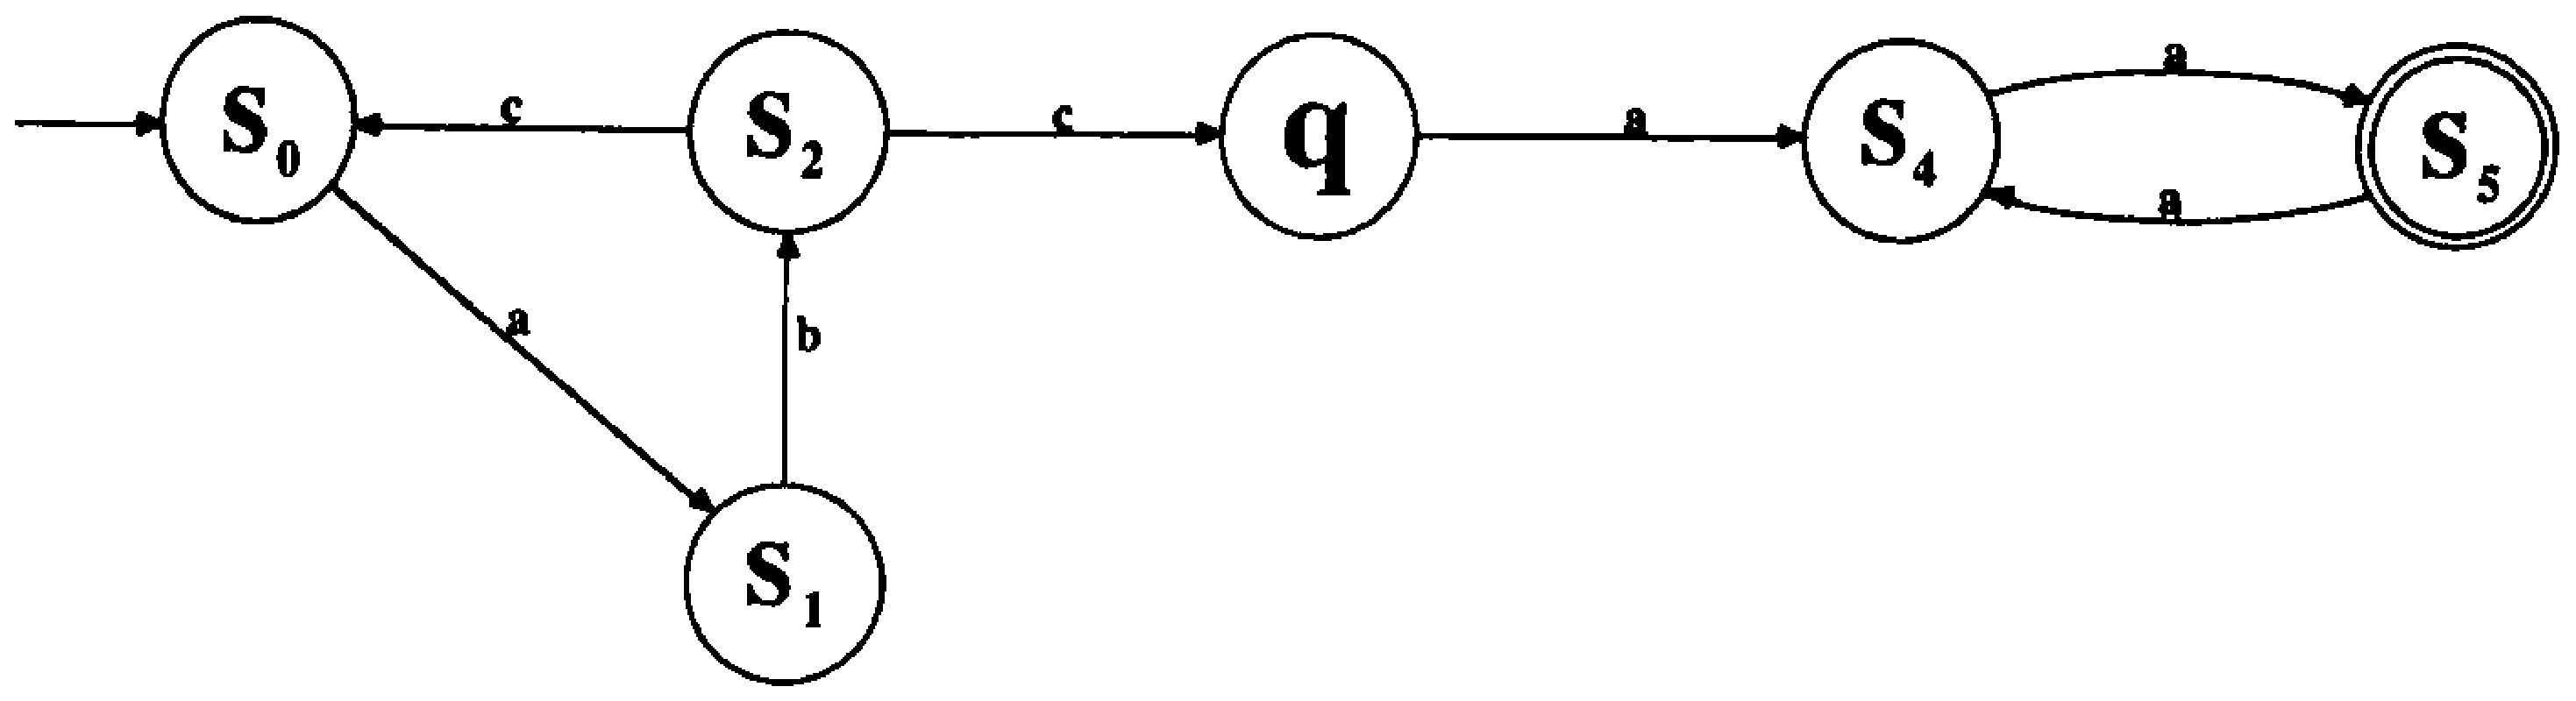
\epsfig{figure=ToFAfigures/fig5-21.eps,width=6in}}
\caption{The automaton discussed in Example 5.25}\label{fig-5.21}
\end{figure}

Similar calculations would have to be done for each of the other states of $A$.
Once again, \NSIG\ does not enjoy the same closure properties that \DSIG\ does.

% Lemma 5.6
\begin{lmm}\label{lmm-5.6}
Let $\Sigma = \{\pmb{a},\pmb{b}\}$.
Then \NSIG\ is not closed under the operator $b$.

\emph{Proof.} Let $L=\{\pmb{a}^n\pmb{b}^n$ $|$ $n \geq 0\}\in \NSIG$. Then $L^b=\{\pmb{a}^n$ $|$ $n\geq 0\}
\notin \NSIG$.
\end{lmm}

Other examples that show \NSIG\ is not closed under the operator $b$ abound. If
$K=\{x\in\{\pmb{a},\pmb{b}\}^*$ $|$ $\ |x|_{\pmb{a}} = |x|_{\pmb{b}}\}$, then
$K^b=\{\pmb{a},\pmb{b}\}^*$. The last operator we will cover in this chapter is
useful for illustrating closures that may not be \emph{effective}, that is, for which
there may not exist an algorithm for constructing the desired entity.
}

% Definition 5.10
\begin{dfn}\label{dfn-5.10}
Let $L_1$ and $L_2$ be languages. The \emph{\Index{quotient}} of $L_1$ with
$L_2$, written $L_1/L_2$, is defined by $L_1/L_2 =\{x$ $|$ $\exists y \in \Sigma^* \ni
y \in L_2 \wedge xy \in L_1\}$
\end{dfn}

Roughly speaking, the quotient consists of the beginnings of those words in
$L_1$ that terminate in a word from $L_2$.

\subsection*{Example 5.26}

Let $\Sigma=\{\pmb{a},\pmb{b}\}$. Then $\{\pmb{b}^2,\pmb{b}^4,\pmb{b}^6,\pmb{b}^8,
\pmb{b}^{10},\pmb{b}^{12},\ldots\}/\{\pmb{b}\}=\{\pmb{b}^1,\pmb{b}^3,\pmb{b}^5,
\pmb{b}^7,\pmb{b}^9,\pmb{b}^{11},\ldots\}$.\\Note that %\linebreak[4]
$\{\pmb{b}^2, \pmb{b}^4, \pmb{b}^6, \pmb{b}^8, \pmb{b}^{10}, \pmb{b}^{12},
\ldots\}/\{\pmb{a}\} = \{\ \}$.

% Theorem 5.12
\begin{thm}\label{thm-5.12}\index{closure!under quotient}
For any alphabet $\Sigma$, \DSIG\ is closed under quotient.

\emph{Proof.} Let $L_1$ and $L_2$ belong to \DSIG. Then there is a
deterministic finite automaton
$A_1=\langle\Sigma,S_1,s_{0_1},\delta_1,F\rangle$ such that $L(A_1)=L_1$. An
automaton that accepts $L_1/L_2$ can be defined by
$A^/=\langle\Sigma,S_1,s_{0_1},\delta_1,F^/\rangle$, where $F^/$ is defined to
be the set of all states $t$ for which there is a word in $L_2$ that reaches a
final state from $t$. That is, $F^/=\{t$ $|$ $\exists y \in \Sigma^*\ni (y \in L_2
\wedge \delta_1(t,y) \in F)\}$. It can be shown that $A^/$ does indeed accept
$L_1/L_2$, and hence \DSIG\ is closed under quotient (see the exercises).
\end{thm}

Note that the above proof did not mention the automaton associated with the
second language $L_2$. Indeed, the definition given for $F^/$ is sufficient to
argue that the new automaton does recognize the quotient of the two languages.
It was not actually necessary to deal with an automaton for $L_2$ in order to
argue that there must exist a DFA that recognizes $L_1/L_2$. The proof of
Theorem \ref{thm-5.12} is thus an \emph{existence} proof, but does not indicate whether
\DSIG\ is \emph{effectively} closed under quotient. Indeed, Theorem \ref{thm-5.12}
actually proves that the quotient of a FAD language with \emph{any} other language
(including those in \NSIG) will always be FAD. However, if it is hard to
determine just which strings in the other language may have the properties we
need to define $F^/$; we may not really know which subset of states $F^/$ should
actually be [after all, we could hardly check the property $\DBAR_1(q,y)\in F$,
one string at a time, for each of an infinite number of strings $y$ in $L_2$ in
a finite amount of time]. Fortunately, it is not necessary to know $F^/$
exactly, since there are only a finite number of ways to choose a set of final
states in the automaton $A^/$, and the proof of Theorem \ref{thm-5.12} assures us that one
of those ways must be the correct one that admits the conclusion
$L(A^/)=L_1/L_2$.

It would, however, be quite convenient to know what $F^/$ actually is so that we
could construct the automaton that actually accepts the quotient; this seems
much more satisfying that just knowing that such a machine must exist! If $L_2$
is FAD, the existence of an automaton
$A_2=\langle\Sigma,S_2,s_{0_2},\delta_2,F_2\rangle$ for which $L(A_2)=L_2$ does
make it possible to calculate $F^/$ exactly (see the exercises). Thus, \DSIG\ is
effectively closed under quotient. In later chapters, languages that may make it
impossible to determine $F^/$ will be studied. We defer the details of such
problems until then.

% Lemma 5.7
\begin{lmm}\label{lmm-5.7}\index{closure!under quotient}
Let $\Sigma=\{\pmb{a},\pmb{b}\}$. \NSIG\ is \emph{not} closed under quotient.

\emph{Proof.} Consider the set $L$ of all strings that have a different number
of $\pmb{a}$s than $\pmb{b}$s. This language is in \NSIG, but $L/L=\Sigma^*$ (why?).
\end{lmm}

From the exercises it will become clear that \NSIG\ is not closed over most of
the usual (or unusual!) operators. Note that \DSIG\ is by contrast a very
special set, in that it appears to be closed over every reasonable unary and
binary operation that we might consider. The question of closure will again
arise as more complex classes of machines and languages are presented in later
chapters.

\section*{Exercises}

\begin{enumerate}[{5.}1. ]
\item Let $\Sigma$ be an alphabet. Define $F_\Sigma$ to be the collection of all
finite languages over $\Sigma$. Prove or give counterexamples to the following:
\begin{enumerate}
\item $\pmb{F_\Sigma}$ is closed under complementation.
\item $\pmb{F_\Sigma}$ is closed under union.
\item $\pmb{F_\Sigma}$ is closed under intersection.
\item $\pmb{F_\Sigma}$ is closed under concatenation.
\item $\pmb{F_\Sigma}$ is closed under Kleene closure.
\item $\pmb{F_\Sigma}$ is closed under relative complement.
\end{enumerate}

\item Let $\Sigma$ be an alphabet. Define $C_\Sigma$ to be the collection of all
 \emph{cofinite}\index{cofinite!collection $C_\Sigma$} languages over $\Sigma$ (a language is cofinite if it is the complement
of a finite language). Prove or give counterexamples to the following:
\begin{enumerate}
\item $\pmb{C_\Sigma}$ is closed under complementation.
\item $\pmb{C_\Sigma}$ is closed under union.
\item $\pmb{C_\Sigma}$ is closed under intersection.
\item $\pmb{C_\Sigma}$ is closed under concatenation.
\item $\pmb{C_\Sigma}$ is closed under Kleene closure.
\item $\pmb{C_\Sigma}$ is closed under relative complement.
\end{enumerate}

\item Let $\Sigma$ be an alphabet. Define $B_\Sigma = F_\Sigma \cup C_\Sigma$
(see Exercises 5.1 and 5.2). Prove or give counterexamples to the following:
\begin{enumerate}
\item $\pmb{B_\Sigma}$ is closed under complementation.
\item $\pmb{B_\Sigma}$ is closed under union.
\item $\pmb{B_\Sigma}$ is closed under intersection.
\item $\pmb{B_\Sigma}$ is closed under concatenation.
\item $\pmb{B_\Sigma}$ is closed under Kleene closure.
\item $\pmb{B_\Sigma}$ is closed under relative complement.
\end{enumerate}

\item Let $\Sigma$ be an alphabet. Define $I_\Sigma$ to be the collection of all
infinite languages over $\Sigma$. Note that $I_\Sigma=\wp(\Sigma^*)-F_\Sigma$
(see Exercise 5.1). Prove or give counterexamples to the following:
\begin{enumerate}
\item $\pmb{I_\Sigma}$ is closed under complementation.
\item $\pmb{I_\Sigma}$ is closed under union.
\item $\pmb{I_\Sigma}$ is closed under intersection.
\item $\pmb{I_\Sigma}$ is closed under concatenation.
\item $\pmb{I_\Sigma}$ is closed under Kleene closure.
\item $\pmb{I_\Sigma}$ is closed under relative complement.
\end{enumerate}

\item Let $\Sigma$ be an alphabet. Define $J_\Sigma$ to be the collection of all
languages over $\Sigma$ that have infinite complements. Note that
$J_\Sigma=\wp(\Sigma^*)-C_\Sigma$ (see Exercise 5.2). Prove or give
counterexamples to the following:
\begin{enumerate}
\item $\pmb{J_\Sigma}$ is closed under complementation.
\item $\pmb{J_\Sigma}$ is closed under union.
\item $\pmb{J_\Sigma}$ is closed under intersection.
\item $\pmb{J_\Sigma}$ is closed under concatenation.
\item $\pmb{J_\Sigma}$ is closed under Kleene closure.
\item $\pmb{J_\Sigma}$ is closed under relative complement.
\end{enumerate}

\item Define $\pmb{E}$ to be the collection of all
languages over $\{\pmb{a},\pmb{b}\}$ that contain the word $\pmb{abba}$. Prove or
give counterexamples to the following:
\begin{enumerate}
\item $\pmb{E}$ is closed under complementation.
\item $\pmb{E}$ is closed under union.
\item $\pmb{E}$ is closed under intersection.
\item $\pmb{E}$ is closed under concatenation.
\item $\pmb{E}$ is closed under Kleene closure.
\item $\pmb{E}$ is closed under relative complement.
\end{enumerate}

\item If a collection of languages is closed under intersection, does it have
to be closed under union? Prove or give a counter example.

\item If a collection of languages is closed under intersection and complement,
does it have to be closed under union? Prove or give a counterexample.

\item Show that if a collection of languages is closed under concatenation it
is not necessarily closed under Kleene closure.

\item Show that if a collection of languages is closed under Kleene closure it
is not necessarily closed under concatenation.

\item Show that if a collection of languages is closed under complementation it
is not necessarily closed under relative complement.

\item Give a finite set of numbers that is closed under $\sqrt{\ \ }$.

\item Give an infinite set of numbers that is closed under $\sqrt{\ \ }$.

\item Given deterministic machines $A_1$ and $A_2$, use the definition of
$A^\cup$ and Definition \ref{dfn-4.5} to describe an algorithm for building a
\emph{deterministic} automaton $A^U$ that will accept $L(A_1) \cup L(A_2)$.

% Can't find how to change symbol size for the "A^\cup"s in (c)
\item Given deterministic machines $A_1$ and $A_2$, and without relying on the
construction used in Theorem \ref{thm-5.2}:
\begin{enumerate}
\item Build a \emph{deterministic} automaton $A^u$ that will accept
$L(A_1) \cup L(A_2)$.
\item Prove that your construction behaves as advertised.
\item If \emph{no} minimization is performed in Exercise 5.14, how do the number of
states in $A^\cup$, $A^U$, and $A^u$ compare? (Assume $A_1$ has $n$ states
and $A_2$ has $m$ states, and give expressions based on these variables.)
\end{enumerate}

\item Let $\Sigma$ be an alphabet. Define the (unary) operator $P$ by
\[ P(L)=\{x\ |\  \exists y \in \Sigma^* \ni xy \in L\}\text{ (for any collection of
words $L$)} \]
$P(L)$ then represents all the \emph{prefixes} of words in $L$. For example, if
$K =\{\pmb{a},\pmb{bbc},\pmb{dd}\}$, then
$P(K)=\{\pmb{\lambda},\pmb{a},\pmb{b},\pmb{bb},\pmb{bbc},\pmb{d},\pmb{dd}\}$. Prove
that \DSIG\ is closed under the operator $P$.

\item Let $\Sigma$ be an alphabet. Define the (unary) operator $S$ by
\[ S(L)=\{x\ | \ \exists y \in \Sigma^* \ni yx \in L\}\text{ (for any collection of
words $L$)} \]
$S(L)$ then represents all the \emph{suffixes} of words in $L$. For example, if
$K=\{\pmb{a},\pmb{bbc},\pmb{dd}\}$, then
$S(K)=\{\pmb{\lambda},\pmb{a},\pmb{c},\pmb{bc},\pmb{bbc},\pmb{d},\pmb{dd}\}$.
\begin{enumerate}
\item Given an automaton accepting $L$, describe how to modify it to produce an
automaton accepting $S(L)$.
\item Prove that your construction behaves as advertised.
\item Argue that \DSIG\ is closed under the operator $S$.
\end{enumerate}

\item Let $\Sigma$ be an alphabet. Define the (unary) operator $C$ by
\[ C(L)=\{x\ | \ \exists y,z \in \Sigma^* \ni yxz \in L\}
	\text{ (for any collection of words $L$)} \]
$C(L)$ then represents all the \emph{centers} of words in $L$. For example, if
$K=\{\pmb{a},\pmb{bbc},\pmb{dd}\}$, then $C(K)=\{\pmb{\lambda},\pmb{a},\pmb{c},
\pmb{bc},\pmb{bbc},\pmb{b},\pmb{bb},\pmb{d},\pmb{dd}\}$.
\begin{enumerate}
\item Given an automaton accepting $L$, describe how to modify it to produce an
automaton accepting $C(L)$.
\item Prove that your construction behaves as advertised.
\item Argue that \DSIG\ is closed under the operator $C$.
\end{enumerate}

\item Let $\Sigma$ be an alphabet. Define the (unary) operator $F$ by
\[ F(L)=\{x\ \ | \ x \in L \wedge (\text{if }\exists y \in \Sigma^* \ni xy \in L,
	\text{then }y = \lambda)\} \]
$F(L)$ then represents all the words in $L$ that are \emph{not} the beginnings of
other words in $L$. For example, if $K=\{\pmb{ad},\pmb{ab},\pmb{abbad}\}$, then
$F(K)=\{\pmb{ad},\pmb{abbad}\}$. Prove that \DSIG\ is closed under the operator
$F$.

\item Let $\Sigma$ be an alphabet, and $x=a_1a_2 \ldots a_{n-1}a_n \in \Sigma^*$;
define $x^r =a_na_{n-1} \ldots a_2a_1$. For a language $L$ over $\Sigma$, define
$L^r=\{x^r$ $|$ $x \in L\}$. Note that the (unary) reversal operator $r$ is thus defined
by $L^r=\{a_na_{n-1} \ldots a_3a_2a_1\ |\ a_1a_2a_3 \ldots a_{n-1}a_n \in L\}$, and
$L^r$ therefore represents all the words in $L$ written backward. For example, if
$K=\{\pmb{\lambda},\pmb{ad},\pmb{bbc},\pmb{bbad}\}$, then
$K^r=\{\pmb{\lambda},\pmb{da},\pmb{cbb},\pmb{dabb}\}$.
\begin{enumerate}
\item Given an automaton accepting L, describe how to modify it to produce an
automaton accepting $L^r$.\index{closure!under reversal}
\item Prove that your construction behaves as advertised.
\item Argue that \DSIG\ is closed under the operator $r$.
\end{enumerate}

\item Let $\Sigma=\{\pmb{a},\pmb{b},\pmb{c},\pmb{d}\}$. Define the (unary)
operator $G$ by
\[ G(L)=\{\pmb{a}_n\pmb{a}_{n-1}\ldots \pmb{a}_3\pmb{a}_2\pmb{a}_1\pmb{a}_1\pmb{a}_2\pmb{a}_3\ldots \pmb{a}_{n-1}\pmb{a}_n\ |\ \pmb{a}_1\pmb{a}_2\pmb{a}_3\ldots
	\pmb{a}_{n-1}\pmb{a}_n \in L\} \]
\[ =\{w^r \cdot w\ |\ w \in L\} \]
(see the definition of $w^r$ in Exercise 5.20). As an example, if
$K=\{\pmb{\lambda},\pmb{ad},\pmb{bbc},\pmb{bbad}\}$, then
$G(K)=\{\pmb{\lambda},\pmb{daad},\pmb{cbbbbc},\pmb{dabbbbad}\}$.
\begin{enumerate}
\item Prove that \DSIG\ is \emph{not} closed under the operator $G$.
\item Prove that \NSIG\ is closed under the operator $G$ (perhaps make use of Theorem \ref{thm-5.11}).
\item Prove that \NSIG\ is not closed under the operator $b$ ($b$ is defined in Theorem \ref{thm-5.11}).
\end{enumerate}

\item Prove that \NSIG\ is closed under the operator $r$ (see Exercise 5.20).\index{closure!under reversal}

\item Prove that \NSIG\ is \emph{not} closed under the operator $P$ (see
Exercise 5.16).

\item Prove that \NSIG\ is \emph{not} closed under the operator $S$ (see
Exercise 5.17).

\item Prove that \NSIG\ is \emph{not} closed under the operator $C$ (see
Exercise 5.18).

\item Prove that \NSIG\ is \emph{not} closed under the operator $F$ (see
Exercise 5.19).

\item Consider the following alternate ``proof'' of Theorem \ref{thm-5.1}: Let $A$ be an
\underline NDFA and define $A^\sim$ as suggested in Theorem \ref{thm-5.1}. Give an example to show
that $L(A^\sim)$ might not be equal to $\sim\!\!L(A)$.

\item Complete the proof of Lemma \ref{lmm-5.7}.

\item Give an example of a collection of languages that is closed under union,
concatenation, and Kleene closure, but is not closed under intersection.

\item If a collection of languages is closed under union, does it have to be
closed under intersection? Prove or give a counterexample.

\item Refer to the construction in Theorem \ref{thm-5.4} and prove that
$L(A^\bullet) = L_1 \cdot L_2$. Warning! This involves a \emph{lot} of tedious details.

\item Refer to the construction in Theorem \ref{thm-5.5} and prove that
$L(A_*) = L^*$. Warning! This involves a \emph{lot} of tedious details.

\item Amplify the explanations for each of the equivalences in the proof of
Theorem \ref{thm-5.2}.

\item Given a DFA $A=\langle\Sigma,S,s_0,\delta,F\rangle$, define an NDFA that
will accept $L(A)^+$.

\item Given an NDFA $A=\langle\Sigma,S,S_0,\delta,F\rangle$, define an NDFA that
will accept $L(A)^+$.

\item If $L$ is FAD, is it necessarily true that all subsets of $L$ are FAD?
Prove or give a counterexample.

\item If $L \in \DSIG$, is it necessarily true that all supersets of $L$ are in
\DSIG? Prove or give a counterexample.

\item If $L \in \NSIG$, is it necessarily true that all subsets of $L$ are in
\NSIG? Prove or give a counterexample.

\item If $L \in \NSIG$, is it necessarily true that all supersets of $L$ are in
\NSIG? Prove or give a counterexample.

\item Explain the purpose of the new start state $q_0$ in the proof of Theorem
\ref{thm-5.5}.

\item Redesign the construction in the proof of Theorem \ref{thm-5.4}, making use of
$\lambda$-transitions where appropriate.

\item Redesign the construction in the proof of Theorem \ref{thm-5.5}, making use of
$\lambda$-transitions where appropriate. Do this in such a way as to make the
``extra'' start state $q_0$ unnecessary.

\item Redesign the construction in the proof of Theorem \ref{thm-5.4}, assuming that $A_1$
and $A_2$ are NDFAs.

\item Redesign the construction in the proof of Theorem \ref{thm-5.5}, assuming that $A$
is a DFA.

\item How does the right congruence generated by a language $L$ compare to the
right congruence generated by the complement of $L$? \emph{Hint:} It may be
helpful to consider the construction of $A^\sim$ given in Theorem \ref{thm-5.1} when $A$
is a minimal machine accepting $L$.

\item \begin{enumerate}
\item Give examples of languages $L_1$ and $L_2$ for which
$R_{(L_1 \cap L_2)} = R_{L_1} \cap R_{L_2}$ (see Definition \ref {dfn-2.2}).
\item Give examples of languages $L_1$ and $L_2$ for which
$R_{(L_1 \cap L_2)} \not= R_{L_1} \cap R_{L_2}$. \emph{Hint:} It may be helpful
to consider the construction of $A^\cap$ given in Lemma \ref{lmm-5.1} to direct your
thinking.
\end{enumerate}

\item Consider the following assertion: \DSIG\ is closed under \emph{relative
complement;} that is, if $L_1$ and $L_2$ are FAD, then $L_1 - L_2$ is also FAD.
\begin{enumerate}
\item Prove this by appealing to existing theorems.
\item Define an appropriate ``new'' machine.
\item Prove that the machine constructed in part (b) behaves as advertised.
\end{enumerate}

\item Define $\mathfrak{L}_\Sigma$ to be the set of all languages recognized by
NDFAs with $\lambda$-transitions. What sort of closure properties does
$\mathfrak{L}_\Sigma$ have? How does $\mathfrak{L}_\Sigma$ compare to \DSIG?

\item \begin{enumerate}
\item Give an example of a language $L$ for which $\lambda \in L^+$.
\item Give three examples of languages $L$ for which $L^+ = L$.
\end{enumerate}

\item Recall that $\delta^\cup$$: (S_1 \cup S_2) \times \Sigma \rightarrow
\wp(S_1 \cup S_2)$ was defined by
\[ \delta^\cup(s,\pmb{a}) = \left\{\begin{tabular}{lrl}
	$\delta_1(s,\pmb{a})$ & if $s \in S_1$ & \\
	& , & $\forall s \in S_1 \cup S_2,\quad \forall\pmb{a} \in \Sigma$ \\
	$\delta_2(s,\pmb{a})$ & if $s \in S_2$ &
	\end{tabular}\right. \]
\begin{enumerate}
\item Prove (by induction) that $\overline{\delta^\cup}$ conforms to a similar formula:
\[ \overline{\delta^\cup}(s,x) = \left\{\begin{tabular}{lrl}
	$\DBAR_1(s,x)$ & if $s \in S_1$ & \\
	& , & $\forall s \in S_1 \cup S_2,\quad \forall x \in \Sigma^*$ \\
	$\DBAR_2(s,x)$ & if $s \in S_2$ &
	\end{tabular}\right. \]
\item Was this fact used in the proof of Theorem \ref{thm-5.2}?
\end{enumerate}

\item Let $\Sigma$ be an alphabet. Prove or give counterexamples to the
following:
\begin{enumerate}
\item \NSIG\ is closed under relative complement.
\item \NSIG\ is closed under union.
\item \NSIG\ is closed under concatenation.
\item \NSIG\ is closed under Kleene closure.
\item If $L \in \NSIG$, then $L^+ \in \NSIG$.
\end{enumerate}

\item Why was it necessary to require that $S_1 \cap S_2 = \emptyset$ in the
proof of Theorem \ref{thm-5.4}? Would any step of the proof be invalid without this
assumption? Explain.

\item Let $\Sigma$ be an alphabet. Define $E(L)=\{z\ |\ (\exists y \in \Sigma^+)
	(\exists x \in L)(z = yx)\}$.
\begin{enumerate}
\item Given an automaton accepting $L$, describe how to modify it to produce an
automaton accepting $E(L)$.
\item Prove that your construction behaves as advertised.
\item Argue that \DSIG\ is closed under the operator $E$.
\end{enumerate}

\item Let $\Sigma$ be an alphabet. Define
$B(L)=\{z\ $ $|$ $(\exists x\in L)(\exists y \in \Sigma^*)(z = xy)\}$.
\begin{enumerate}
\item Given an automaton accepting $L$, describe how to modify it to produce an
automaton accepting $B(L)$.
\item Prove that your construction behaves as advertised.
\item Argue that \DSIG\ is closed under the operator $B$.
\end{enumerate}

\item Let $\Sigma$ be an alphabet. Define
$M(L)=\{z\ $ $|$ $(\exists x \in L)(\exists y \in \Sigma^+)(z = xy)\}$.
\begin{enumerate}
\item Given an automaton accepting $L$. describe how to modify it to produce an
automaton accepting $M(L)$.
\item Prove that your construction behaves as advertised.
\item Argue that \DSIG\ is closed under the operator $M$.
\end{enumerate}

\item Refer to the definitions given in Lemma \ref{lmm-5.1} and use induction to show
that
\[ (\forall s \in S_1)(\forall t \in S_2)(\forall x \in \Sigma^*)(\overline{\delta^\cap}
	(\langle s,t\rangle,x) = \langle\DBAR_1(s,x),\DBAR_2(t,x)\rangle ) \]

\item Refer to Lemma \ref{lmm-5.1} and prove that $L(A^\cap)=L_1 \cap L_2$. As long as the
reference is explicitly stated, the result in Exercise 5.56 can be used without
proof.

\item Prove Theorem \ref{thm-5.6}.

\item Prove Theorem \ref{thm-5.7}.

\item \begin{enumerate}
\item Cleverly define a machine modification that does not use any
$\lambda$-moves that could be used to prove Theorem \ref{thm-5.7} (your new machine is
still likely to be nondeterministic, however).
\item Prove that your modified machine behaves as advertised.
\end{enumerate}

\item Let $W(L)=\{x\ $ $|$ $x$ is formed by deleting one or more letters from a word
in L$\}$.
\begin{enumerate}
\item Given an automaton accepting $L$, describe how to modify it to produce an
automaton accepting $W(L)$.
\item Prove that your construction behaves as advertised.
\item Argue that \DSIG\ is closed under the operator $W$.
\end{enumerate}

\item Let $V(L)=\{x $ $|$ $x$ is formed by deleting the odd-positioned letters from a
word in $L\}$. [\emph{Note:} This refers to the first, third, fifth, and so on,
letters in a word. For example, if $\pmb{abcdefg}\in L$, then $\pmb{bdf}\in
V(L)$.]
\begin{enumerate}
\item Given an automaton accepting $L$, describe how to modify it to produce an
automaton accepting $V(L)$.
\item Prove that your construction behaves as advertised.
\item Argue that \DSIG\ is closed under the operator $V$.
\end{enumerate}

\item Let $U(L)=\{x\ $ $|$ $x$ is formed by deleting the even-positioned letters from
a word in $L\}$. [\emph{Note:} This refers to the second, fourth, sixth, and so
on, letters in a word. For example, if $\pmb{abcdefg} \in L$, then
$\pmb{aceg} \in U(L)$.]
\begin{enumerate}
\item Given an automaton accepting $L$, describe how to modify it to produce an
automaton accepting $U(L)$.
\item Prove that your construction behaves as advertised.
\item Argue that \DSIG\ is closed under the operator U.
\end{enumerate}

\item Let $T(L)=\{x\ $ $|$ $x$ is formed by deleting every third, sixth, ninth, and so
on, letters from a word in $L\}$. [\emph{Note:} This refers to those letters in
a word whose index position is congruent to $0 \bmod{3}$. For example, if
$\pmb{abcdefg} \in L$, then $\pmb{abdeg} \in T(L)$.]
\begin{enumerate}
\item Given an automaton accepting $L$, describe how to modify it to produce an
automaton accepting $T(L)$.
\item Prove that your construction behaves as advertised.
\item Argue that \DSIG\ is closed under the operator $T$.
\end{enumerate}

\item For any alphabet $\Sigma$,
let $P=\{x\in\Sigma^*$ $|$ $|x|$ is prime$\}$ and let $I(L)$ be defined by
$I(L) = L \cap P$.
\begin{enumerate}
\item Show that \DSIG\ is not closed under $I$.
\item Show that $F_\Sigma$ is closed under $I$ (see Exercise 5.1).
\item Prove or disprove: $C_\Sigma$ is closed under $I$ (see Exercise 5.2).
\item Prove or disprove: $B_\Sigma$ is closed under $I$ (see Exercise 5.3).
\item Prove or disprove: $I_\Sigma$ is closed under $I$ (see Exercise 5.4).
\item Prove or disprove: $J_\Sigma$ is closed under $I$ (see Exercise 5.5).
\item Prove or disprove: $E$ is closed under $I$ (see Exercise 5.6).
\item Prove or disprove: \NSIG\ is closed under $I$.
\end{enumerate}

\item Define $C$ to be the collection of all languages over
$\{\pmb{a},\pmb{b}\}$ that do not contain $\lambda$. Prove or give
counterexamples to the following:
\begin{enumerate}
\item $C$ is closed under complementation.
\item $C$ is closed under union.
\item $C$ is closed under intersection.
\item $C$ is closed under concatenation.
\item $C$ is closed under Kleene closure.
\item $C$ is closed under relative complement.
\item If $L \in C$, then $L^+ \in C$
\end{enumerate}

\item \begin{enumerate}
\item Consider the statement that \DSIG\ is closed under finite union:
\begin{enumerate}
\item Prove by existing theorems and induction.
\item Prove by construction.
\end{enumerate}
\item Prove or disprove that \DSIG\ is closed under infinite union. Justify your
assertions.
\end{enumerate}

\item Let $\Sigma =\{\pmb{a},\pmb{b}\}$.
\begin{enumerate}
\item Give examples of three homomorphisms under which \NSIG\ is not closed.
\item Give examples of three homomorphisms under which \NSIG\ is closed.
\end{enumerate}

\item Let $\Sigma =\{\pmb{a}\}$. Can you find two different homomorphisms under
which \NSIG\ is not closed? Justify your conclusions.

\item Refer to the construction given in Theorem \ref{thm-5.10}.
\begin{enumerate}
\item Prove $\overline{\delta^{\psi}}\!(s,x)=\DBAR(s,\PBAR(x)) \forall s \in S,\forall x \in
	\Sigma^*$
\item Complete the proof of Theorem \ref{thm-5.10}.
\end{enumerate}

\item Consider the homomorphism $\xi$ given in Lemma \ref{lmm-5.4} and the set $L$ of all
strings that have the same number of $\pmb{a}$s as $\pmb{b}$s.
\begin{enumerate}
\item \DSIG\ is closed under inverse homomorphism, but $\xi(L)$ is the set of
all even-length strings of $\pmb{a}$s, and it appears that under
$\overline{\xi^{-1}}$ the DFA language $\xi(L)$ maps to the non-FAD language $L$.
Explain the apparent contradiction. \emph{Hint:} First compute
$\overline{\xi^{-1}}(\xi(L))$
\item Give an example of a homomorphism for which $\PBAR(\overline{\psi^{-1}}(L)) \not= L$.
\item Give an example of a homomorphism for which $\overline{\psi^{-1}}(\PBAR(L)) \not= L$.
\item Prove $\PBAR(\overline{\psi^{-1}}(L)) \subseteq L$.
\item Prove $L \subseteq \overline{\psi^{-1}}(\PBAR(L))$.
\end{enumerate}

\item Let $\Sigma$ be an alphabet. Define the (unary) operator $e$ by
\[ L^e=\{x\ | \ \exists y \in \Sigma^* \ni (yx \in L \wedge |x|=|y|)\} \]
$L^e$ then represents the last halves of all the words in $L$. For example, if
$K=\{\pmb{ad},\pmb{abaa},\pmb{ccccc}\}$, then $K^e=\{\pmb{d},\pmb{aa}\}$. Prove
that \DSIG\ is closed under the operator $e$.

\item Refer to the proof of Theorem \ref{thm-5.11} and show that there exists an automaton
$A$ for which it would be incorrect to try to accept $L^b$ by redefining the set
of final states to be merely the set of ``midway'' states.

\item Consider the sets $M$ and $K$ in Example 5.20. Assume that we have used
the pumping lemma to show that $M$ is not FAD. What would be wrong with arguing
that, since $M$ was not FAD, its homomorphic image cannot be FAD either, and
hence $K$ is therefore not FAD.

\item Prove Theorem \ref{thm-5.9}.

\item Let $\Sigma$ be the ASCII alphabet. Define a homomorphism that will
capitalize all lowercase letters (and does not change punctuation, spelling, and
the like).

\item Consider the proof of Theorem \ref{thm-5.12}.
\begin{enumerate}
\item Show that
$L(A^{^/}) = L_1/L_2$
for the $A$ and $A^{^/}$ defined by
$A=\langle\Sigma,S_1,s_{0_1},\delta_1,F\rangle$ and
$A^{^/}=\langle\Sigma,S_1,s_{0_1},\delta_1,F{^/}\rangle$, where
$ F^{^/} =\{t\ | \ \exists y \in \Sigma^* \ni (y \in L_2 \wedge \DBAR_1(t,y) \in F)\}$.
\item Given deterministic finite automata
$A_1=\langle\Sigma,S_1,s_{0_1},\delta_1,F\rangle$ such that $L(A_1) = L_1$,
and $A_2=\langle\Sigma,S_2,s_{0_2},\delta_2,F_2\rangle$ for which $L(A_2) = L_2$,
give an algorithm for computing $F^{^/}=\{t$ $|$ $\exists y \in \Sigma^* \ni (y \in L_2
\wedge \DBAR_1(t,y) \in F)\}$.
\end{enumerate}

\item Given two alphabets $\Sigma_1$ and $\Sigma_2$ and a DFA
$A=\langle\Sigma_1,S,s_0,\delta,F\rangle$:
\begin{enumerate}
\item Define a new automaton $A'=\langle\Sigma_1 \cup \Sigma_2,S',s_0',\delta',
F'\rangle$ for which $L(A')=L(A)$.
\item Prove that $A'$ behaves as advertised.
\end{enumerate}

\item Let $S$ be a collection of languages that is closed under union,
concatenation, and Kleene closure. Prove or disprove: If $S$ contains an
infinite number of languages, every language in $S$ must be FAD.

\item Let $S$ be a collection of languages that is closed under union,
concatenation, and Kleene closure. Prove or disprove: If $S$ is a finite
collection, every language in $S$ must be FAD.

\item Let $u$ be a unary language operator that, when composed with itself,
yields the identity function. Prove that if \DSIG\ is closed under $u$,
then \NSIG\ must also be closed under $u$.
\end{enumerate}
